\documentclass{pennThesis}

%%--------------------------------------------------------------------
%% preamble
%%--------------------------------------------------------------------

\title{A Search for the Higgs boson produced in association with top quarks in multilepton final states at ATLAS}
    
\author{Chris Lester}

\newcommand{\adviser}{I. Joseph Kroll, Professor, Physics}
\newcommand{\advisershort}{Joseph Kroll}

\newcommand{\myinstitution}{The Univeristy of Pennsylvania}

\newcommand{\chairperson}{Elliot Lipeles, Associate Professor, Physics}

\newcommand{\committeeOne}{Justin Khoury, Associate Professor, Physics}
\newcommand{\committeeTwo}{I. Joseph Kroll, Professor, Physics}
\newcommand{\committeeThree}{Burt Ovrut, Professor, Physics}
\newcommand{\committeeFour}{Evelyn Thompson, Associate Professor, Physics}
\draftversion{00-01}

\newboolean{springer}
\setboolean{springer}{false}



%% feynmf for feynman diagrams
\usepackage{feynmf}
\setlength{\unitlength}{1mm}

%% other std packages
\usepackage{multirow}
%\usepackage{multicol}
%\usepackage{rotating}
%\usepackage{morefloats}

%% personal style files

%% to temporarily include only a single chapter
%%--------------------------------------------------------------------
%% begin the document
%%--------------------------------------------------------------------
\begin{document}
\begin{fmffile}{thesis-feyn}

\def \etrel {$E_{\rm T}Cone20/p_{\rm T}$~}
\def \ptrel {$p_{\rm T}Cone20/p_{\rm T}$~}
\def \htjet {H_{\mathrm{T}}}
\def \pt {$p_{\mathrm{T}}$}
\def \et {E_{\mathrm{T}}}
\def \ee {$e^{\pm}e^{\pm}$~}
\def \emu {$e^{\pm}\mu^{\pm}$~}
\def \mumu {$\mu^{\pm}\mu^{\pm}$~}


\newcommand{\Wj}{{$W$+jets}~} 
\newcommand{\W}{$W^{\pm}$~} 
\newcommand{\WW}{$W^{+}W^{-}$~} 
\newcommand{\WZ}{$W^{\pm}Z$} 
\newcommand{\SWW}{$W^{\pm}W^{\pm}$~} 
\newcommand{\twotau}{$\tau^{+}\tau^{-}$~} 
\newcommand{\ZZ}{$ZZ$~} 
\newcommand{\tth}{$t\bar{t}H$} 
\newcommand{\ttV}{$t\bar{t}V$} 
\newcommand{\tZ}{$tZ$} 
\newcommand{\ttW}{$t\bar{t}W^{\pm}$} 
\newcommand{\ttWW}{$t\bar{t}W^{\pm}W^{\pm}$~} 
\newcommand{\ttZ}{$t\bar{t}Z$} 
\newcommand{\hww}{$H\rightarrow W^+W^-$~} 
\newcommand{\hzz}{$H\rightarrow ZZ$~} 
\newcommand{\htt}{$H\rightarrow \tau^+\tau^-$~} 
\newcommand{\Wb}{$W^{\pm}b$~} 
\newcommand{\taupm}{$\tau^{\pm}$~} 
\newcommand{\zj}{{$Z$+jets}~} 
\newcommand{\zg}{{$Z\gamma$}~} 
\newcommand{\wg}{{$W^{\pm}\gamma$}~} 
\newcommand{\lumi}{$\mathcal{L}$~} 
\newcommand{\btt}{\ttbar background~} 
\newcommand{\hzzstar}{$H\rightarrow ZZ^*$~}

%%--------------------------------------------------------------------
%% title page
%% copyright
%% acknowledgements
%% abstract
%%--------------------------------------------------------------------
\frontmatter
\maketitle

%%--------------------------------------------------------------------
%% table of contents
%% list of tables
%% list of figures
%%--------------------------------------------------------------------
\begin{Spacing}{\mylinespacing}
\tableofcontents
\end{Spacing}
\clearpage

%% let the list of tables and figures use the default single-spacing
% TODO: uncomment these when you are ready
\listoftables
\clearpage
\listoffigures
\clearpage

%%--------------------------------------------------------------------
%% preface
%%--------------------------------------------------------------------
\begin{Spacing}{\mylinespacing}

\chapter*{Preface}
\addcontentsline{toc}{chapter}{Preface}

This is the preface.  Blah blah blah blah blah blah blah.
Blah blah blah blah blah blah blah.  Blah blah blah blah blah blah blah.
Blah blah blah blah blah blah blah.  Blah blah blah blah blah blah blah.
Blah blah blah blah blah blah blah.  Blah blah blah blah blah blah blah.
Blah blah blah blah blah blah blah.  Blah blah blah blah blah blah blah.
Blah blah blah blah blah blah blah.  Blah blah blah blah blah blah blah.
Blah blah blah blah blah blah blah.  Blah blah blah blah blah blah blah.
Blah blah blah blah blah blah blah.  Blah blah blah blah blah blah blah.

Blah blah blah blah blah blah blah.  Blah blah blah blah blah blah blah.
Blah blah blah blah blah blah blah.  Blah blah blah blah blah blah blah.
Blah blah blah blah blah blah blah.  Blah blah blah blah blah blah blah.
Blah blah blah blah blah blah blah.  Blah blah blah blah blah blah blah.
Blah blah blah blah blah blah blah.  Blah blah blah blah blah blah blah.
Blah blah blah blah blah blah blah.  Blah blah blah blah blah blah blah.
Blah blah blah blah blah blah blah.  Blah blah blah blah blah blah blah.

\vspace{0.05\textheight}

\begin{tabular}{p{0.5\textwidth} l}
  & Ryan Reece            \\
  & CERN, December 2012   \\
\end{tabular}



%%--------------------------------------------------------------------
%% main sections
%%--------------------------------------------------------------------
\mainmatter
%% \chapter[htoc-titlei][hhead-titlei]{htitlei}
%% -----------------------------------------------------------------------------
\chapter[Introduction][Introduction]{Introduction}

The discovery of the Higgs boson at the Large Hadron Collider (LHC) experiments has opened up a new paradigm of research into the
Standard Model of particle physics.
This thesis primarily documents a search for the production of Higgs boson in association with top quarks (\tth) 
in multi-lepton final states.  Searching for this production mode of the Higgs is an important
step toward a precise measurement of the top Yukawa coupling, because it accesses this coupling via diagrams
that do not contain loops. Comparison of this coupling with the already well-measured top quark mass provides
a direct test of a fundamental provision of the Higgs mechanism: that it gives mass to the fermions. 

The analysis uses the 2012 ATLAS experiment's dataset of proton-proton collisions at 
a center-of-mass energy of 8 TeV provided by the LHC. The statistics available do not allow for an observation of the \tth\ process
at the Standard Model production cross-section, and the results of the search are interpreted as
a 95\% exclusion on the production rate. The results will provide some of strictest constraints on the rate to date and
establish a program for future analyses on larger datasets that will eventually observe this production mode. 

Chapter~\ref{chapter:theory} provides theoretical background and motivation for the study of this particular
Higgs production mode and Chapter~\ref{chapter:lhc} provides a basic review of the experimental apparatus,
the LHC and ATLAS. Chapter~\ref{chapter:electron} is a brief diversion
from the main text to elaborate on the techniques used to identify electrons and measure their identification
efficiency. 

Chapters~\ref{chapter:analysis - chapter:results} are the main text, which discuss the full analysis
procedure for the search and the final measurement. The results of the analysis are currently undergoing approval
in the ATLAS collaboration and eventually will be documented for publication. Once approved the results
will be combined with other Higgs searches to set limits on Higgs couplings to other SM particles,
particularly the top quark. 

%% \chapter[htoc-titlei][hhead-titlei]{htitlei}
%% -----------------------------------------------------------------------------
\chapter[Theoretical Background][Theoretical Background]{Theoretical Background}

The Standard Model of particle physics (SM) is an extraordinarily successful
description of the fundamental constituents of matter and their interactions.
Many experiments have verified the extremely precise
prediction of the SM. This success has culminated most recently in the
discovery of the Higgs Boson.  This chapter provides a brief introduction to
the structure of the SM and how scientists are able to test it using hadron
collider. It focuses primarily on the physics of the Higgs boson and its decays
to top quarks.  I stress the importance of a
measurement of the rate at which Higgs Bosons are produced in association of
top quarks, as a new, rigorous test of the SM. The experimental search
for this production mode in multi-lepton final states is the 
general subject of this thesis.


\section{The Standard Model}
\subsection{The Standard Model Structure}

The Standard Model (SM) \cite{np_22_579, prl_19_1264, 1964.Salam-Ward.gauge-theory,1973.Weinberg.SM-with-QCD} is an example of a quantum field theory that describes
the interactions of all of the known fundamental particles. Particles are understood to be excitations of the more fundamental
object of the theory, the field. The dynamics and interactions of the fields are
derived from the Standard Model Lagrangian, which is constructed to be
symmetric under transformations of the group $SU(3) \times SU(2)_L
  \times U(1)$. $SU(3)$ is the group for the color, $SU(2)_L$ is the group 
for weak iso spin, and $U(1)$ is the group for weak hyper-charge.

Demanding these symmetries be local, gauge symmetries allows the theory to be
re-normalizable \cite{1972.tHooft-Veltman.regularization_and_renormalization}, meaning that unwanted infinities can be absorbed into
observables from theory in a way that allows the theory to be able to predict
physics at multiple energy scales.
Gauging the symmetries results in the introduction of 8 massless gluons, or the
boson\footnote{bosons are full integer spin particles that obey Bose-Einstein statistics, while fermions are half-integer spin particles that obey Fermi-Dirac statistics} carriers of the strong force \cite{1973.Gross-Wilczek.Asymptotic_freedom_0} from the generators
$SU(3)$ symmetry, and the 4 massless bosons, carriers for the weak
and electromagnetic forces from the 3 generators of the $SU(2)$ and 1
generator of the $U(1)$ group. The weak and the electromagnetic forces are considered part of a larger single 
unified electroweak group $SU(2) \times U(1)$ and the associated generators mix. 

Matter particles are fermion particles, definied as represenations of the symmetry groups. Singlets of the $SU(3)$ 
are called leptons, do not have a color charge, and, therefore, do not interact with the strong force. Quarks,
on the other hand, are triplets of the $SU(3)$ group do interact with the strong force. The SM is a chiral theory:
the weak force violates parity, as it only couples to left-chiral particles or right-chiral antiparticles. 
This means that right-chiral and left-chiral fermions arise from different fields, which are
different representations of the $SU(2)_L$ group.
 
The discovery of particles and new interactions in various experiments
is intertwined with the development of the theory that spans many
decades and is not discussed in detail here. But these
experiments have proven the above model and symmetries to be an overwhemlimg success.
So far, 3 separate generations of both quarks and leptons have been discovered, differing only by mass. The gluons and the 4 electroweak bosons have also been discovered($W^+$, $W^-$, $Z^0$, and $\gamma$). The reason for this 3-fold replication is not known. Figure~\ref{figure:theory_sm} shows a table of the known SM particle content.  


\begin{figure}[!t]
\centering 
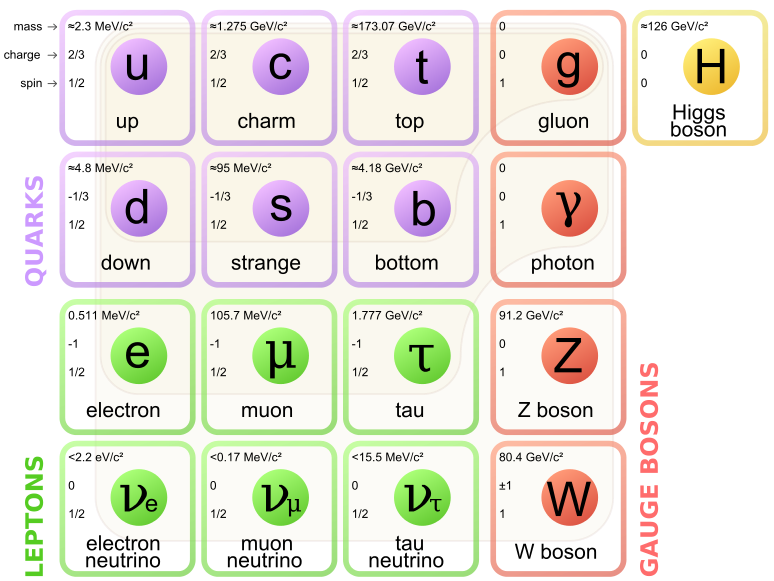
\includegraphics[width=0.9\textwidth]{figs/theory/iaGJO.png}
\caption{ The Standard Model Particle Content
 } \label{figure:theory_sm}
\end{figure}


\subsection{Electroweak Symmetry Breaking and the Higgs}

Despite the simple structure of theory, the discovery of massive fundamental
particles creates two sets of problems both related to $SU(2)_{L} \times U(1)$ symmetry. First, the force-carrying bosons must enter the theory
without mass or the symmetries will be explicitly broken in the Lagrangian. Second, adding
fermion masses to theory in an ad-hoc way allows the right-chiral and
left-chiral fermions to mix. Since they possesses different quantum numbers, as
different representations of the weak-isospin group, this too breaks gauge
invariance. 

To solve these problems, spontaneous electro-weak symmetry breaking (EWSB) is
introduced via the Brout-Englert-Higgs mechanism \cite{Higgs:1964pj, Higgs:1966ev,Englert:1964et}. A  massive scalar field
in an electro-weak doublet is added to the theory with 4 new
degrees of freedom and a potential which includes a 
quartic self-interaction term. Each fermion field interacts with the scalar field via
a different Yukawa coupling, which unites the left and right chiral fields
of a single particle type.  This field
explicitly preserves all of the symmetries, but the minimum of the potential does not
occur when the expectation of the field is zero. The field
eventually falls to a state, where it acquires a non-zero vacuum-expectation
value. A non-vanishing field must point in a
particular direction of weak-isospin space, breaking the symmetry.

The consequences of this spontaneous symmetry breaking are tremendous.
The universe is filled with a field that has a non-zero expectation value.
The theory can be expanded around this new value and 3 of the
degrees of freedom can be interpreted as the longitudinal polarizations of
the $W^+$, $W^-$, and $Z^0$, while the 4th remains a scalar field, called
the Higgs field with an associated particle called the Higgs particle or "Higgs".
The weak bosons acquire a mass via their longitudinal polarizations and the Yukawa
couplings of the scalar field to the fermions now behave like a mass term
at the this new minimum. 


\subsection{The Standard Model Parameters}


Confronting the SM with experiment requires the measurement of
17\footnote{There are additional parameters from neutrino mass terms and
mixing but it is unclear how to include these into the Standard Model,
since it does not predict right-chiral neutrinos} free parameters, which
are unconstrained from the theory. These free parameters include the fermion
masses from the Yukawa couplings, the force coupling constants, the angles and phase of the mixing between
quarks, and constants from the Higgs and electroweak sector\footnote{ The electroweak sector includes
parameters like mass of the $W^{\pm}$ and $Z^0$ bosons, the weak mixing
angle,${\mathrm sin^2}\theta_w$, the fermi constant $G_F$, and Higgs
Mass and vacuum expectation value. These parameters however are not
wholly independent. As discussed above, it is only necessary
theoretically to specify the two parameters relevant to the Higgs
potential and the two coupling associated with the gauge groups }.

%arXiv:1209.2716v2%
Experiments have provided a number of measurements of the
parameters of the SM\cite{lepew:2010vi}.  With the discovery of the Higgs boson and 
the measurement of the Higgs mass, all of the parameters
of the SM can be estimated and statistical procedures can assess
the relative agreement of overlapping measurements to test the self-consistency 
of the SM. The GFitter collaboration assembles
all relevant electroweak observable measurements into a statistical
model and then allows certain measurements to float within their
uncertainty to allow for a fit among multiple correlated measurements\cite{GFitter}. 
These correlations arise for two reasons. First, measurments are made that often
depend on multiple SM parameters. Second, radiative corrections often cause 
parameters to depend on each other. For instance, the Higgs mass is sensitive
to both the $W$ mass and top mass, through loop level corrections. 

Figure \ref{figure:theory_scans} shows the fitted constraints on 4 key SM
parameters ($M_H$, $M_W$, $M_t$, ${\mathrm sin^2}\theta_w$) with
actual measurements overlaid. The plots show both the removal
and inclusion in the fit of key measurements to assess their overall
impact. The addition to the fit of the measured
Higgs mass from the ATLAS and CMS collaborations creates a small
tension, as the other observables prefer the mass to be much
lower ($\sim$ 80 GeV). This tension in the combined
electroweak fit as a result is  not statistically
significant with a $p$-value of 0.07. The
SM seems to be self-consistent. 


\begin{figure}[!t]
\centering 
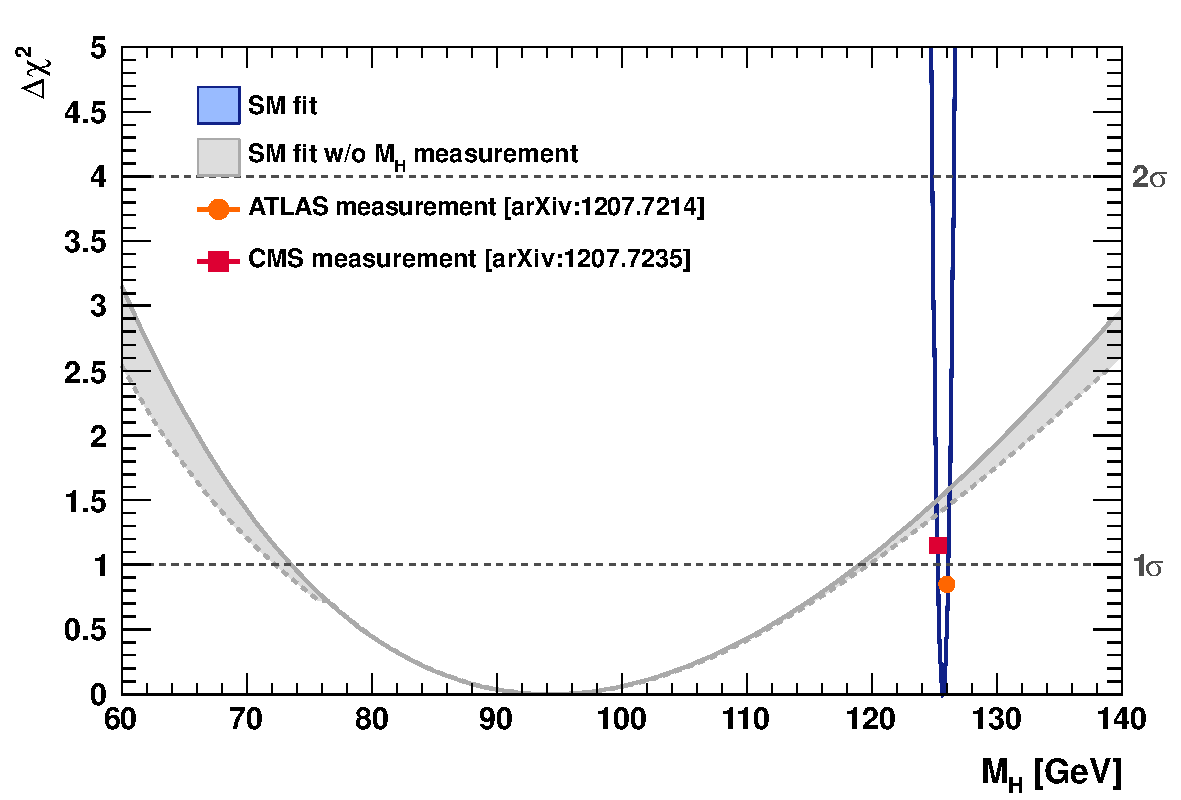
\includegraphics[width=0.45\textwidth]{figs/theory/HiggsScan.pdf}
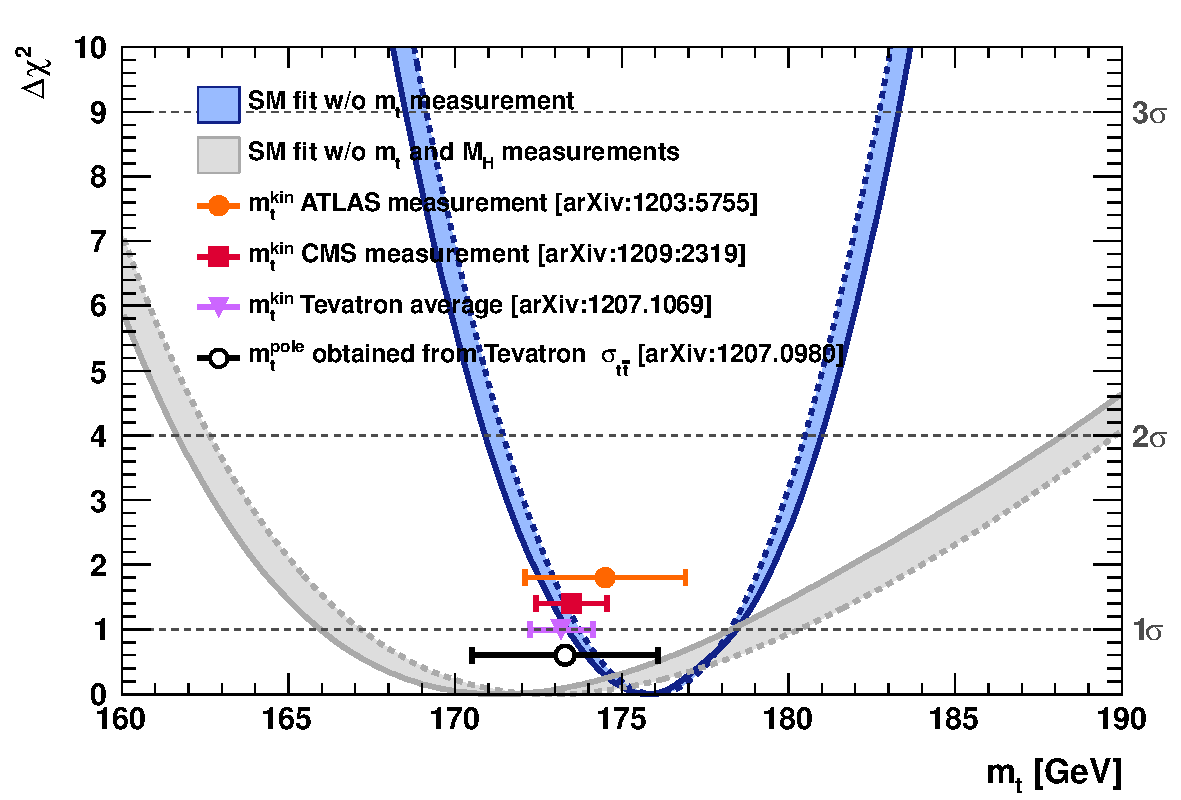
\includegraphics[width=0.45\textwidth]{figs/theory/TopScan.pdf}
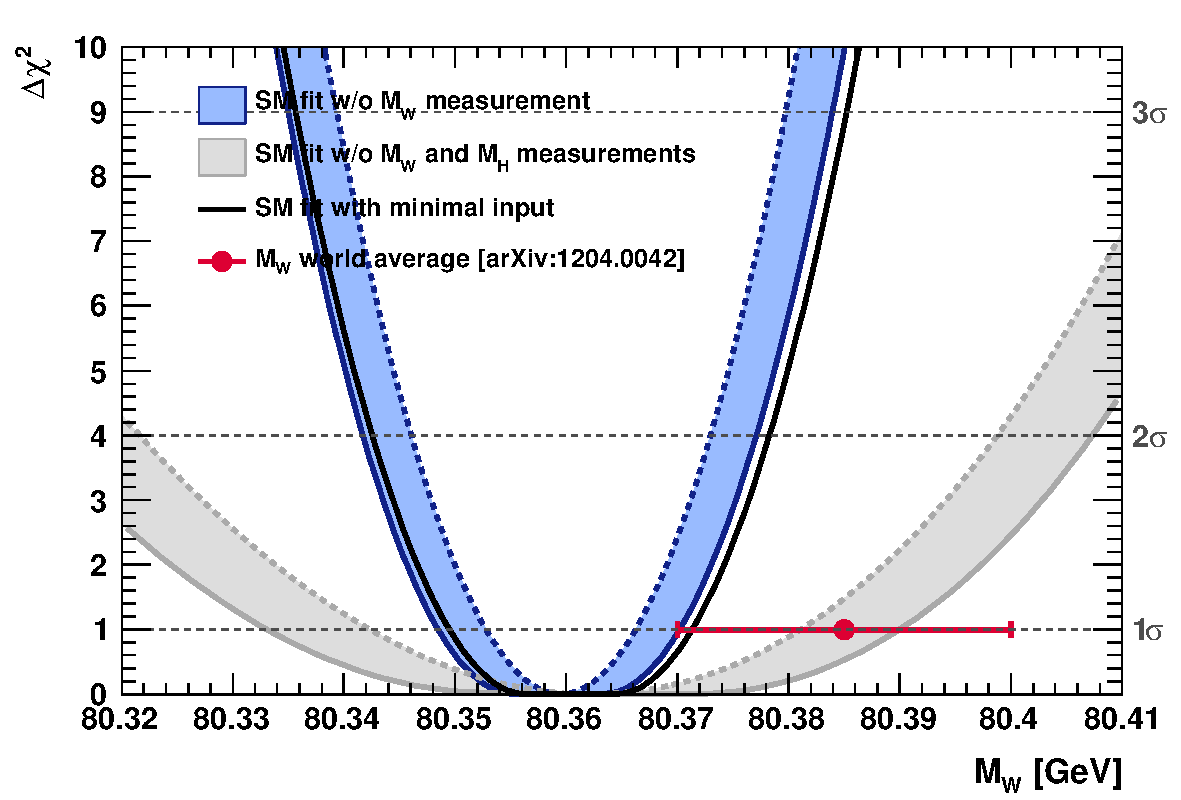
\includegraphics[width=0.45\textwidth]{figs/theory/WMassScan.pdf}
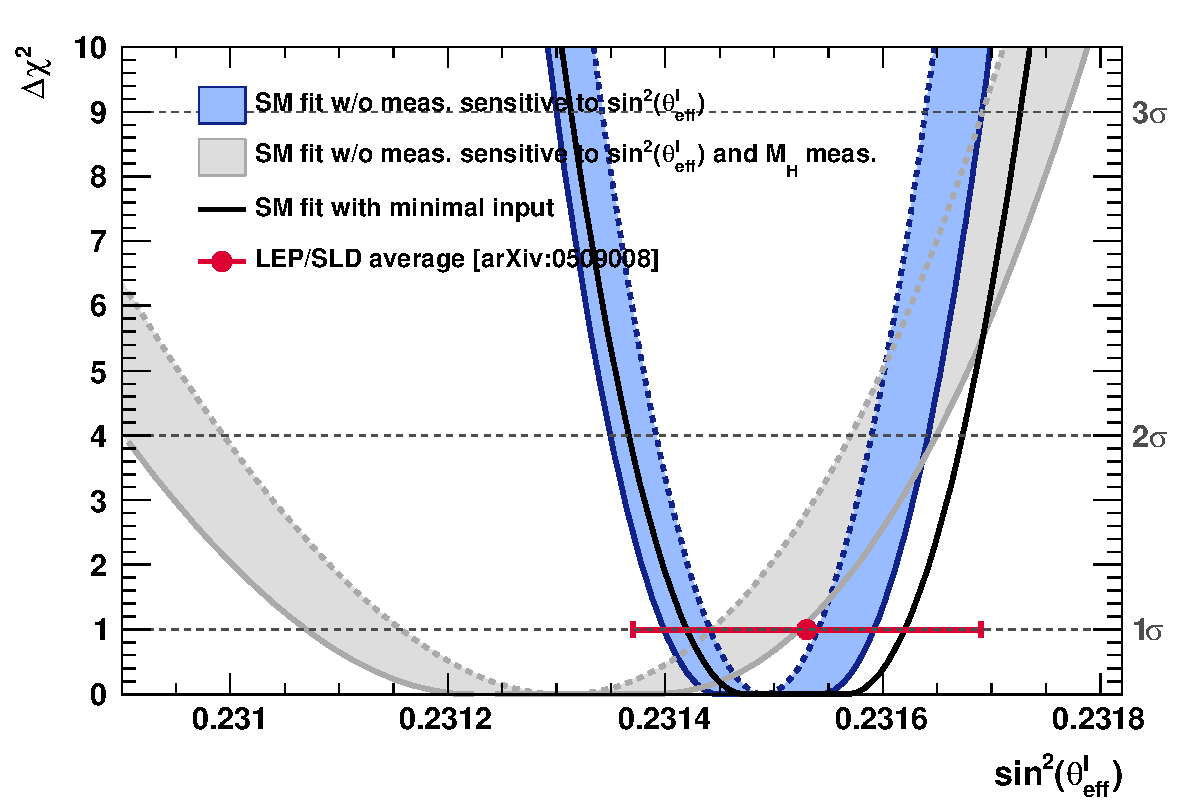
\includegraphics[width=0.45\textwidth]{figs/theory/Sin2ThetaScan.pdf}
\caption{
$\chi^2$ as a function of the Higgs mass (top left), the top quark mass (top
    right), the $W$ boson mass (bottom left) and the effective weak mixing
  angle (bottom right) for the combined SM fit from the GFitter group.  The
  data points placed along $\chi^2=1$ represent direct measurements of the
  respective observable and their $\pm 1\sigma$ uncertainties.  The grey (blue)
  bands show the results when excluding (including) the new $M_H$ measurements
  from (in) the fits. } \label{figure:theory_scans}
\end{figure}


\section{Collider Physics and the Higgs} 

To test the theory, physicists accelerate particles to extremely high energies and force
them to interact through collisions. Typically, the particles accelerated are
electrons or protons, since they are stable. Electron-positron collider
machines have a rich history of discovery and measurement in particle physics.
The advantage of electron accelerators is that the colliding element is itself
a fundamental particle. However, due to synchrotron radiation, the curvature of the
beam line becomes problematic for high energy beams.  On the other
hand, proton-proton and proton-anti-proton colliders can be accelerated in rings without large losses
due to synchrotron radiation, but the actual colliding objects at high
energies are the constituent quarks and gluons. This complicates analysis
because the initial state of the hard-scattering system is not known on a per-collision
basis and momentum of hard-scattering system is unknown along the beam direction.

For hadron colliders, physicists must rely on form-factor descriptions of the colliding hadrons
that describe the fraction of momentum carried by the
hadrons constituent 'partons'.  These are called parton-distribution
functions, seen in Figure \ref{figure:theory_pdf}, and are factorized
and integrated through the theoretical calculations of various collision processes \cite{1985.Collins.factorization-theorem}.

%http://arxiv.org/pdf/0901.0002v3.pdf
At the Large Hadron Collider or LHC, the collider used in this thesis, protons are collider.The types of initial hard-scattering statesat the LHC are quark-quark, quark-gluon, and gluon-gluon. Gluon collisions dominate overall,
  due to the large number of gluons inside the proton, though the relative importance of different initial states changes with the
  energy scale of the collision and the type of final state sought after.  

\begin{figure}[!t]
\centering 
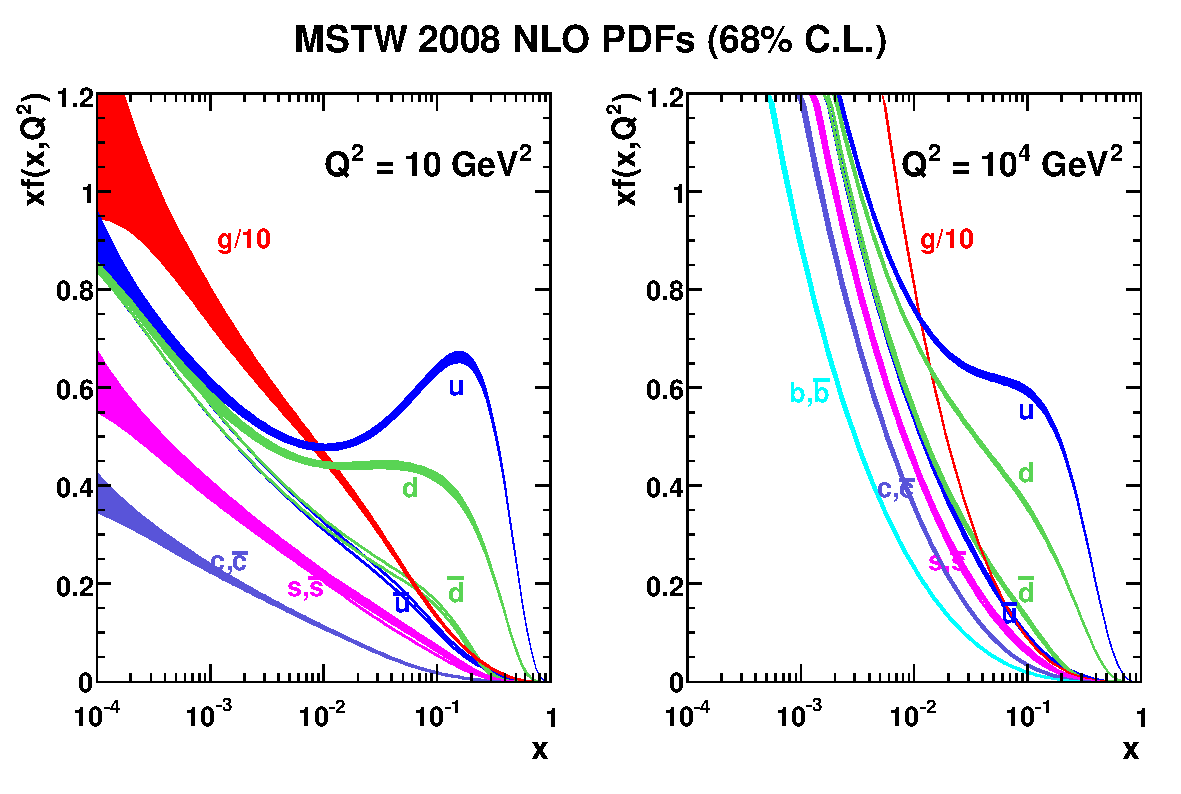
\includegraphics[width=0.8\textwidth]{figs/theory/mstw2008nlo68cl_allpdfs.pdf}
\caption {Proton Parton Distribution Functions (PDFs) form the MSTW Collaboration at $Q^2 = 10$ GeV$^2$ and $Q^2 = 10^4$ GeV$^2$}.
\label{figure:theory_pdf}
\end{figure}

%

%
A prime motivation for the construction of the Large Hadron Collider was the
discovery or exclusion of the Higgs boson\cite{lhcProposal}. LEP and the Tevatron excluded large
swaths of possible Higgs boson masses, especially below 114 GeV. The Higgs mass was also known to 
have a theoretically motivated upper bound. The unitarity of diagrams including the $WWWW$ vertex required the Higgs mass to
be below about 1 TeV.This LHC was thus designed to be able to eventually find or exclude 
a Higgs particle in this range \cite{lepew:2010vi}. 

Reaching this discovery oor exclusion required an enormous
dataset with collisions at high energies. Despite the fact that the Higgs couples to nearly
every particle, Higgs boson production at the LHC is a
low rate process. Because it couples to fermions proportional to mass and
because the colliding particles must be stable and therefore light, production
of the Higgs must occur through virtual states. 

\begin{figure}[!t]
\centering
\begin{tabular}{cc}
\subfloat[ggF]{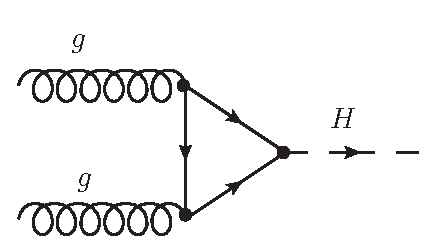
\includegraphics[width=0.35\textwidth]{figs/theory/ggF.pdf}} &
\subfloat[vbf]{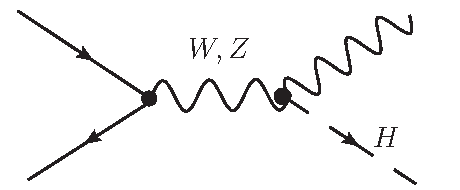
\includegraphics[width=0.35\textwidth]{figs/theory/vh.pdf}} \\
\subfloat[vh]{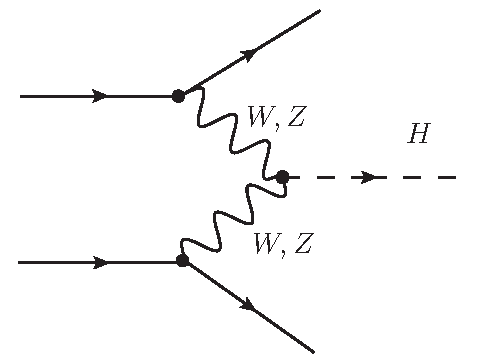
\includegraphics[width=0.35\textwidth]{figs/theory/vbf.pdf}} &
\subfloat[$t\bar{t}H$]{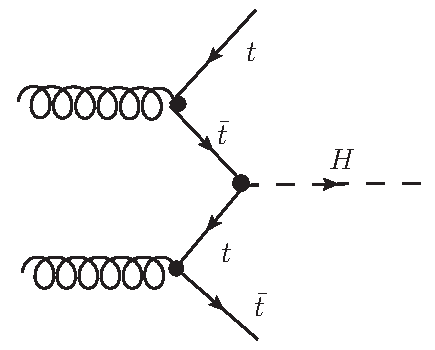
\includegraphics[width=0.35\textwidth]{figs/theory/tth.pdf}} \\
\end{tabular} 
\caption{Dominant Higgs production modes at the LHC}
\label{figure:theory_higgsdiagrams}
\end{figure}


The Higgs boson can be produced through collision at the LHC
via 4 mechanisms: gluon-fusion (ggF), vector-boson fusion (VBF), 
Higgsstrahlung (VH), and production in association with top quarks ($t\bar{t}H$). The diagrams
are shown in Figure \ref{figure:theory_higgsdiagrams} and the production
cross-sections as a function of Higgs mass for the 8 TeV LHC proton-proton
running are shown in Figure \ref{figure:theory_xsec} \cite{Dittmaier:2012vm}. The largest production
cross-section is via the gluon fusion channel at ~$20$ pb, which proceeds
through a fermion loop that is dominated by the top quark, because of its
large Yukawa coupling to the Higgs. Because the Higgs' couples to every massive
particle, it has a rich set of decays also seen in Figure
\ref{figure:theory_xsec}, especially for $m_H=125$.  Studies of Higgs
properties at hadron colliders offers many tests of the Standard Model
and ample room for searches for new physics. These
tests specifically can verify the link between Yukawa coupling and the
particles mass and further constrain details of EWSB by examining Higgs coupling
to the weak bosons. 

\begin{figure}[!t]
\centering 
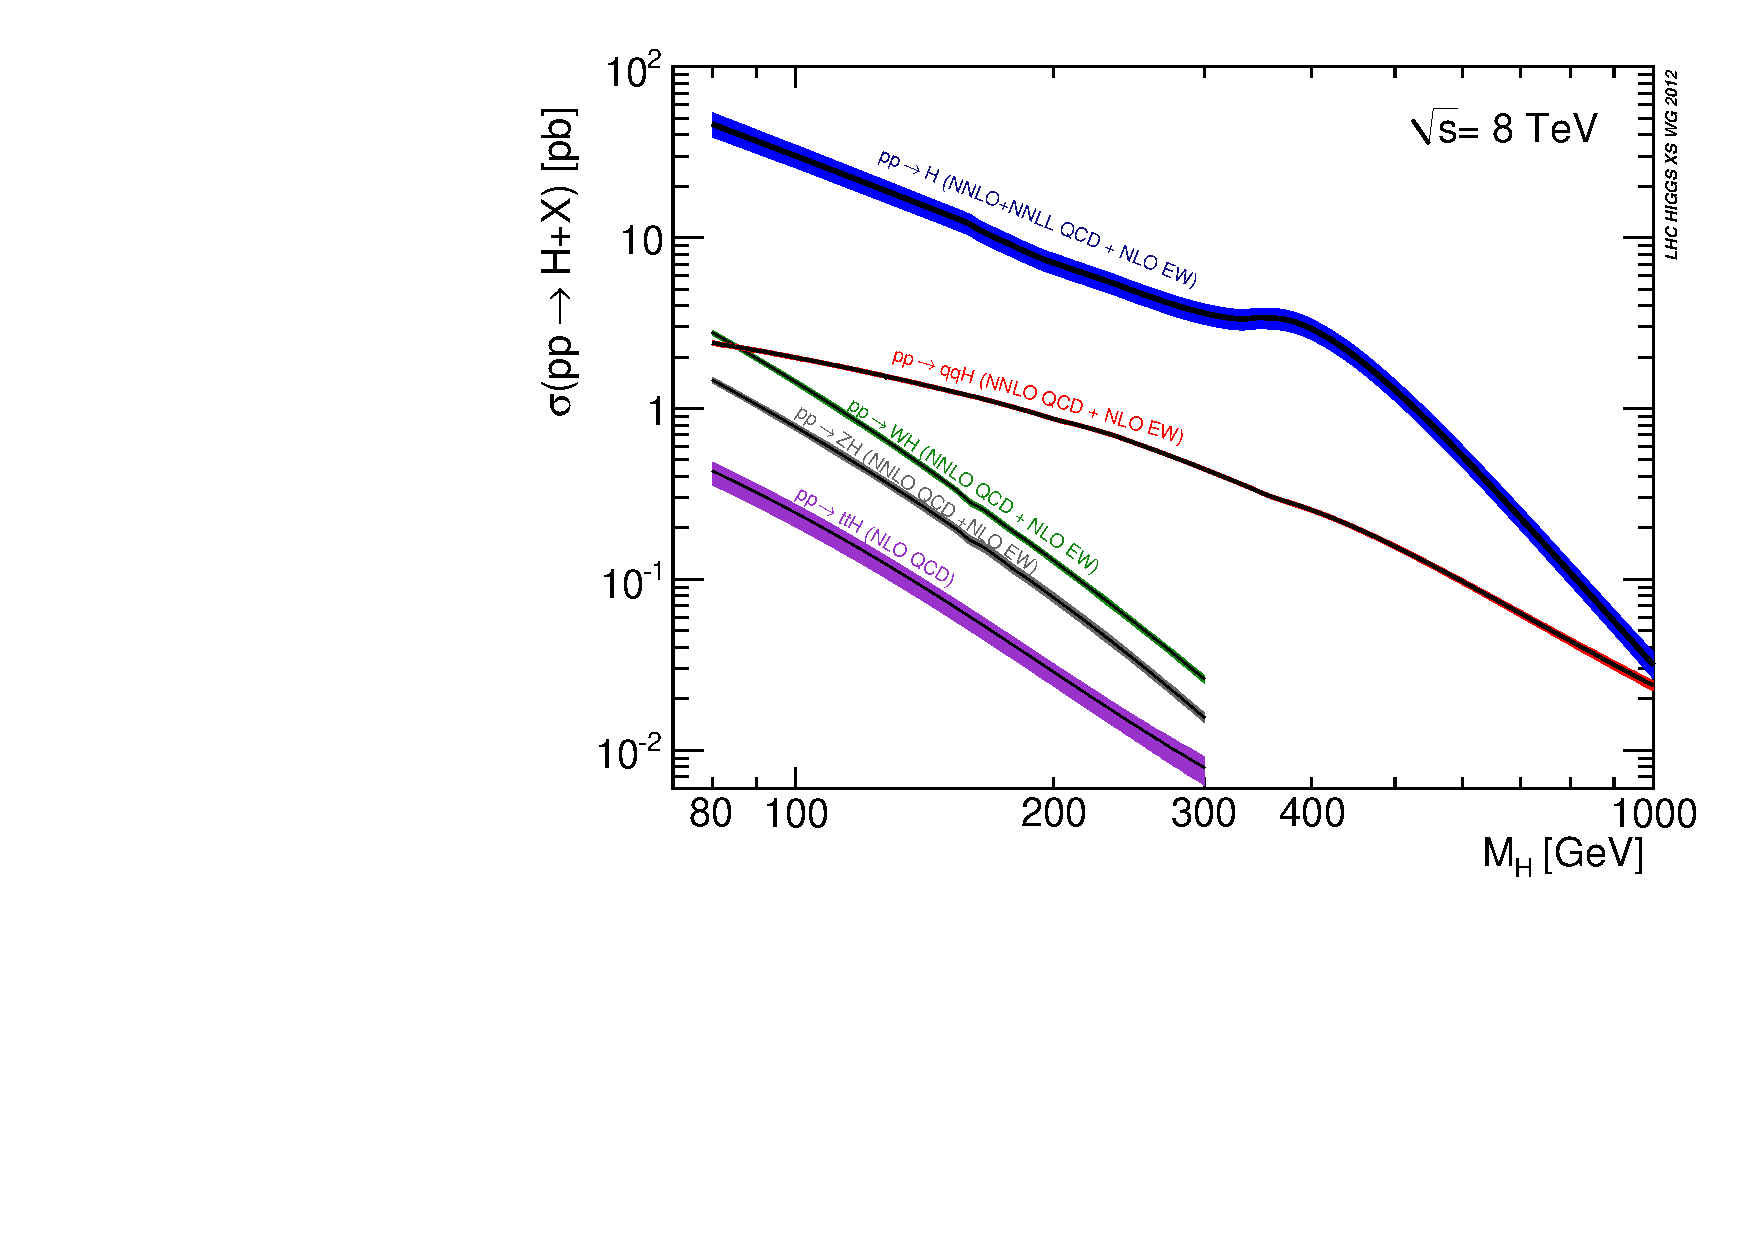
\includegraphics[width=0.52\textwidth]{figs/theory/Higgs_XS_8TeV_lx.pdf}
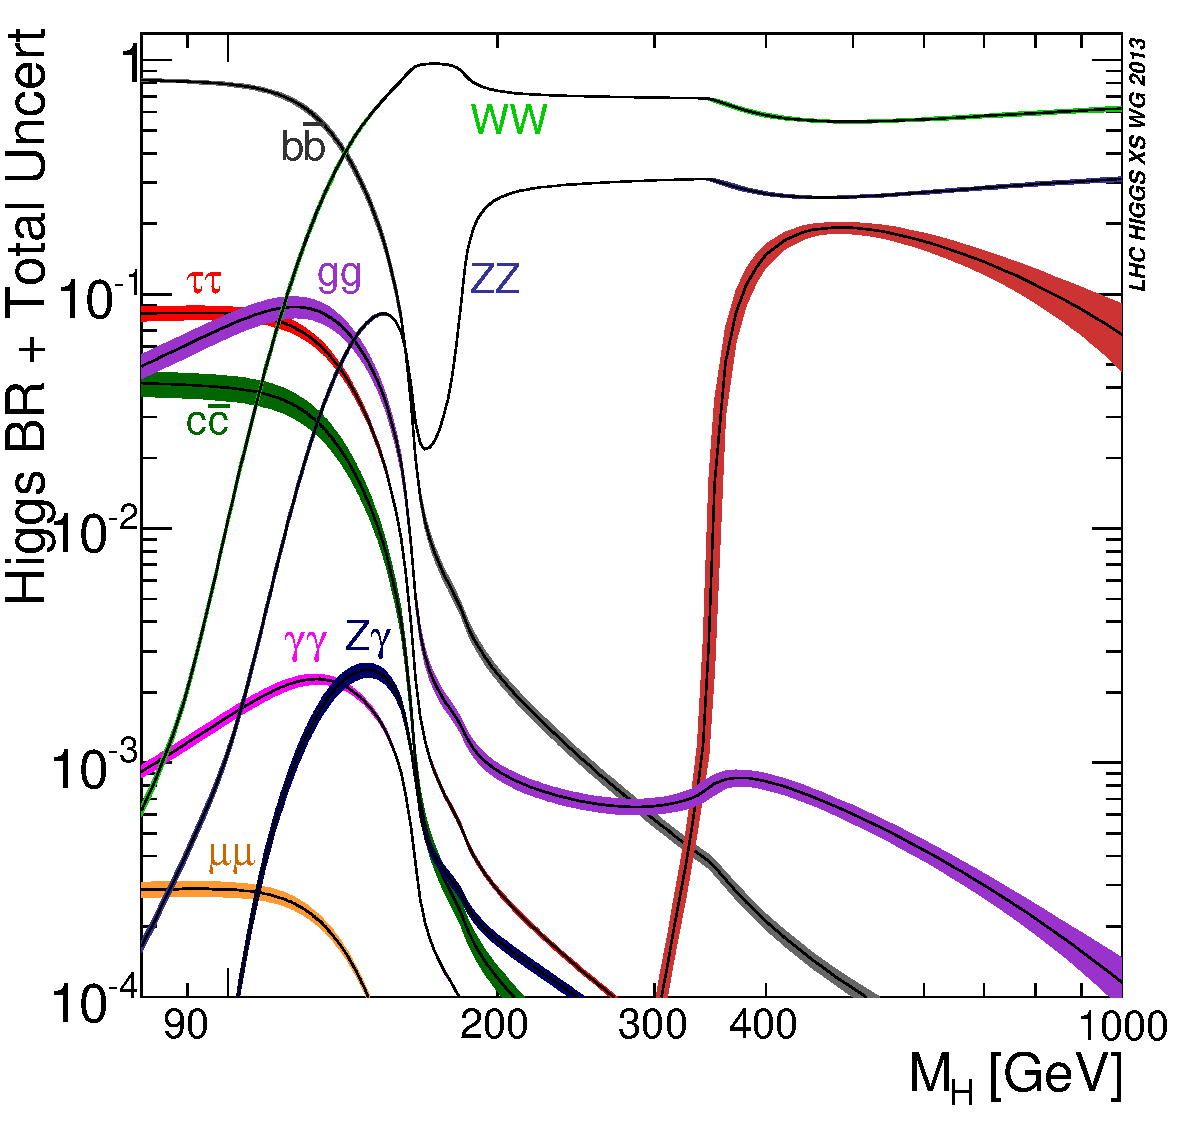
\includegraphics[width=0.42\textwidth]{figs/theory/Higgs_BR.pdf}
\caption {8 TeV LHC Higgs production cross-sections (left) and decay branching fractions }.
\label{figure:theory_xsec}
\end{figure}


\subsection{Higgs Discovery at the LHC}

In 2012 both ATLAS and CMS announced the discovery of a new boson consistent
with the Higgs by examining the results of Higgs searches in a number of decay
channels ($H\rightarrow W^+W^-$,$H\rightarrow Z^0Z^0$, and
    $H\rightarrow\gamma\gamma$) in the 2011 dataset at $\sqrt{s}=$7 TeV and
part of the 2012 dataset at $\sqrt{s}=$8 TeV. By 2013 and 2014, both
experiments have updated and/or finalized their results for the full 2011 and
2012 datasets \cite{ATLAS-CONF-2014-009,CMS-PAS-HIG-14-009}. I will focus on the ATLAS results in the following. 
ATLAS measured both the Higgs mass\cite{Aad:2014aba} and spin\cite{tagkey2013120}, as well as 
provided initial constraints of the Higgs couplings to different particles. 

Figure \ref{figure:theory_higgsdisc} show the results of the searches in all of the
measurement channels as well as constraints on the SM Higgs coupling parameters in 
an example fit, where the couplings to the top-quark, bottom-quark, W,Z, and $\tau$
are allowed to fluctuate independently. These rely on measurements binned in different
production and decay channels. They are dominated by higher statistics results in the 
gluon-fusion production modes, but measurements in the VH and VBF modes are close to 
SM sensitivity. 

The combined results show basic agreement with the SM with much room for improvement
with the addition of new production and decay modes and higher statistics. The 
coupling constraints are particularly strong for the W and Z, which are
the most sensitive decay channels, and top quark due to the dominance of the
top Yukawa in the ggF loop. 


\begin{figure}[!t]
\centering 
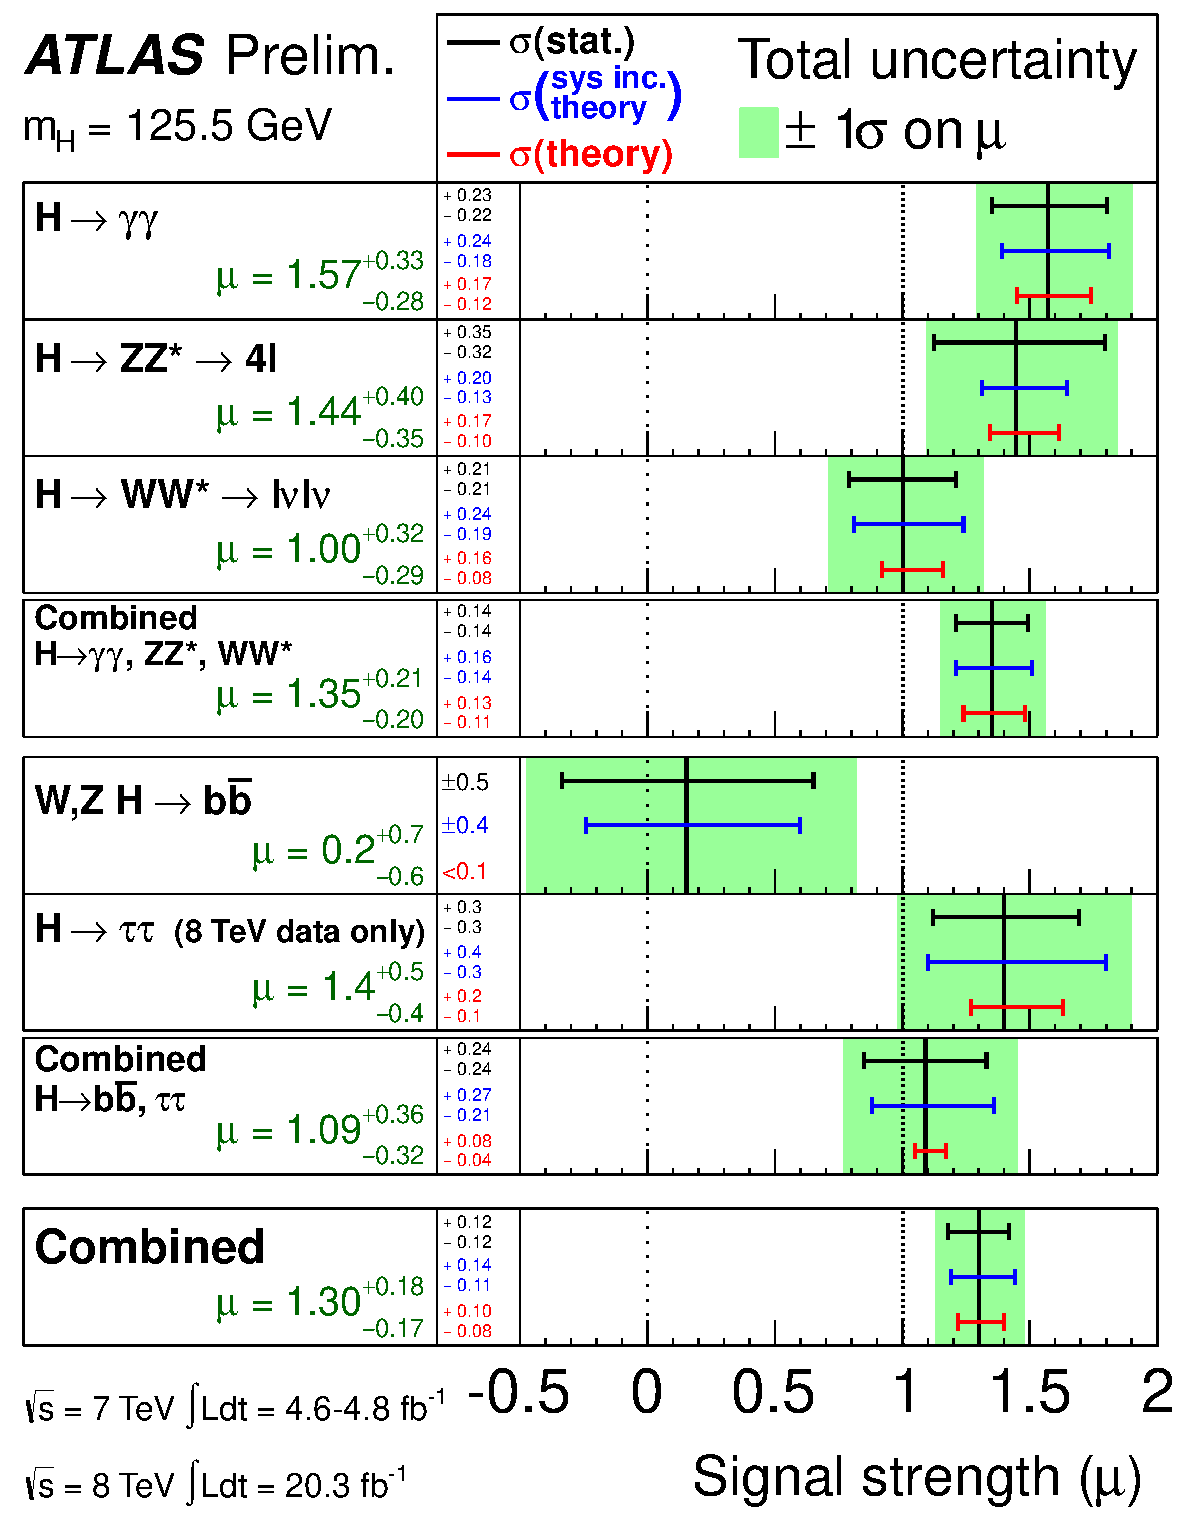
\includegraphics[width=0.45\textwidth]{figs/theory/atlas_higgs.pdf}
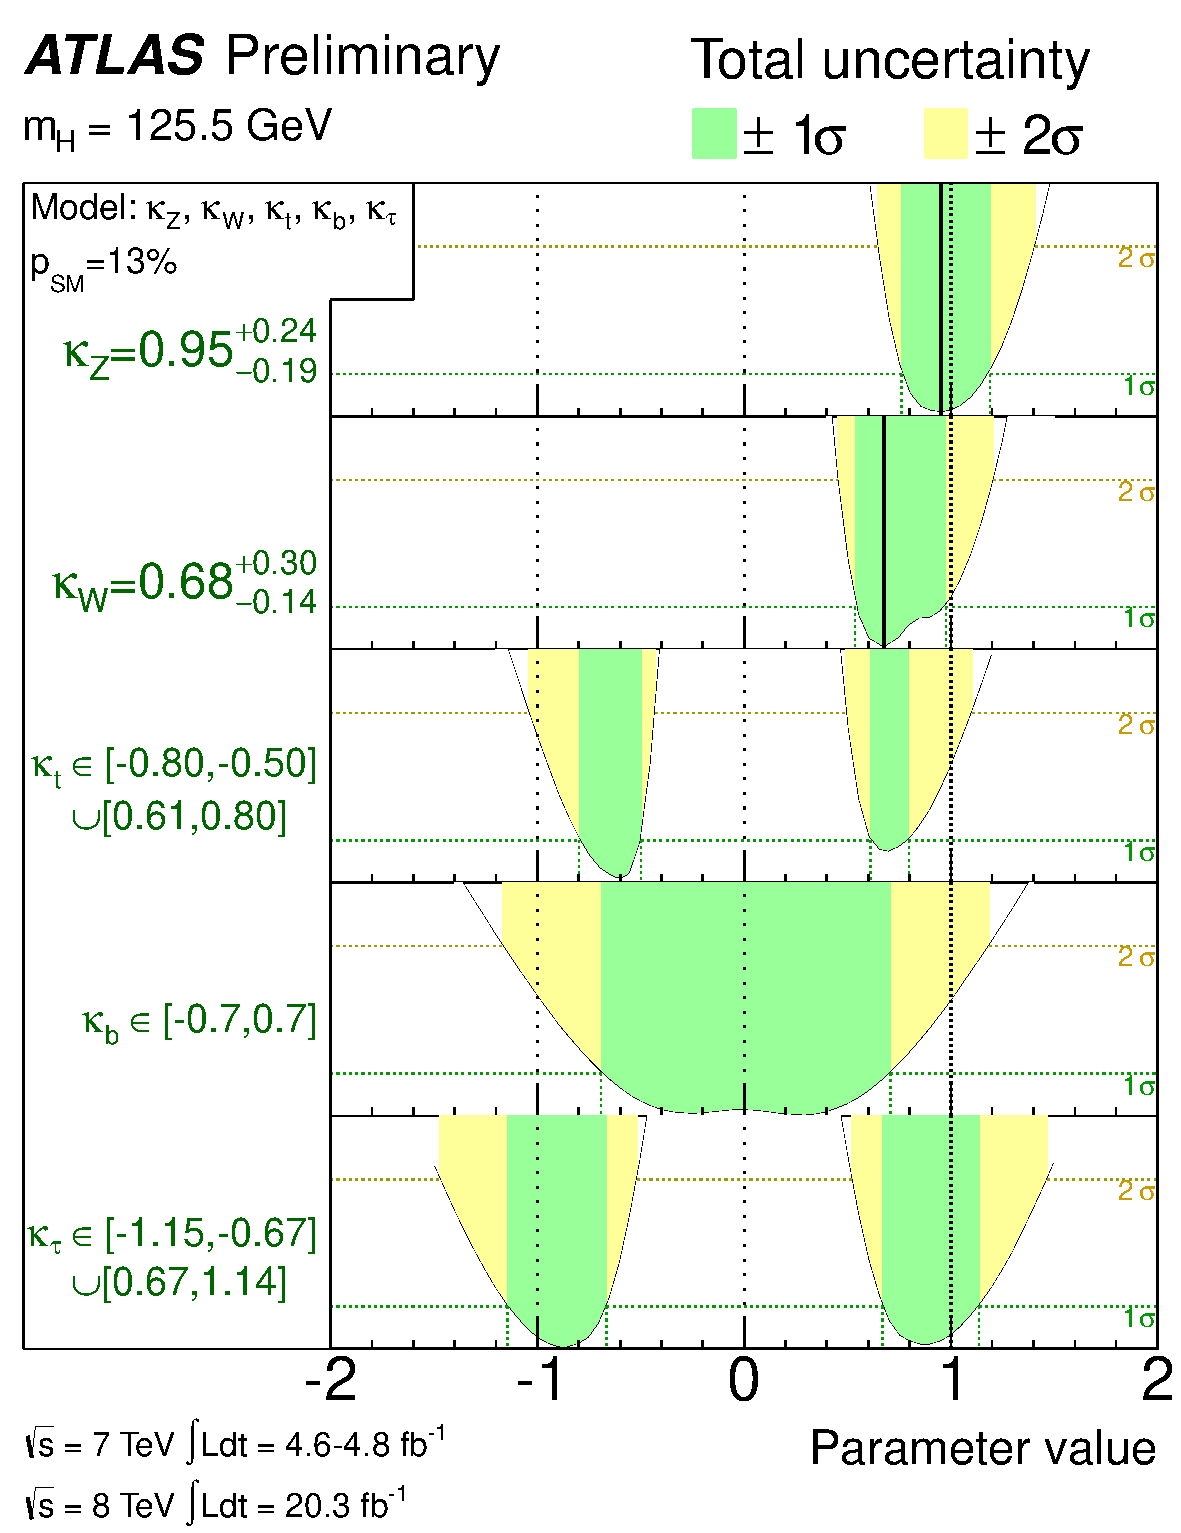
\includegraphics[width=0.45\textwidth]{figs/theory/atlas_coupling.pdf}
\caption {
  ATLAS Higgs combination results for all SM measurement channels as ratios of
  the measured to SM production cross-sections (left) and extracted Higgs
  coupling constraint scale-factors for a combined fit to the measurement
  channels, where the W,Z, top-quark, b-quark, and $\tau$ couplings are
  allowed to float. The p-value of this particular model is 0.13 and in agreement
  with SM expectations}

\label{figure:theory_higgsdisc}
\end{figure}


\subsection{The Importance $t\bar{t}H$ Production}

Notably absent thus far in the SM are searches for the Higgs in the $t\bar{t}H$
production channel, due to the low production rate and lack of statistics. Searches are underway and
initial results are close to SM sensitivity for ATLAS and CMS.

Measuring the $t\bar{t}H$ production rate is important, because
$t\bar{t}H$ production depends on the top Yukawa coupling at tree level. Comparing
the predicted Yukawa coupling from top mass measurements to the coupling from
the wholly independent Higgs production measurements is a very direct 
test of Higgs' invovlment in providing mass the fermions in the SM.

The top Yukawa coupling is already constrained from current measurements of the ggF production
process, since ggF loop is dominated by the top quark. However, new, colored particled could be
present in the loop. Comparison of the gluon-fusion and the $t\bar{t}H$
modes would allow for disentangling the effects of these possible new particles\cite{Dawson:2013bba}. 
The simplest of new phyiscs models, allowing for the modification
of the ggF loop, introduce a new generation of quarks. However, fourth
generation quarks, which obtain mass from a Higgs Yukawa coupling, are already
largely excluded due to their enormous effects on the Higgs production
cross-section\cite{Eberhardt:2012gv}. Other exotic scenarios allow for new colored particles, 
which are not entirely constrained by present measurements\cite{Carena:2013iba,ArkaniHamed:2012kq,Carmi:2012yp}.
These include, for instance, supersymmetric models involving the stop quark.  

With the level of statistics available in Run I dataset, very strict constraints on the top 
Yukawa coupling are simply not possible and the measurment presented in this 
thesis is a first stemp. Future, high-statistics datasets will have the ability to provide 
better measurments and \tth production will become very important.
Despite similar uncertainties on the overall production cross-sections for $t\bar{t}H$ and the ggF,
\tth has the advantage that most of these uncertainties would cancel for $t\bar{t}H$ if normalized to the topologically similar $t\bar{t}Z$.  Finally, the uniqueness of the experimental signature means that
searches for $t\bar{t}$ signatures can be performed for a variety of Higgs decays ($\gamma\gamma$, $b\bar{b}$,
$WW$,$ZZ$, and $\tau\bar{\tau}$ with roughly similar degrees of sensitivity (within a factor of 10)\cite{Dawson:2013bba}. 


It is important to note the importance of the top Yukawa coupling
due to its enormous size compared to other couplings. For instance, the top Yukawa is 350000x as large as the electron
Yukawa coupling. The top Yukawa coupling,
along with the Higgs mass, is one of the most important pieces of the renormalization group equations (RGE)
responsible for the running of the parameter that determines the Higgs self-coupling $\lambda$. 
If this parameter runs negative, then the potential responsible for the entire mechanism 
of EWSB no longer has a minimum and becomes unbounded, resulting in instability in the universe \cite{Degrassi:2012ry}.
Metastability occurs when the shape of the potential allows for a false local minimum.
Figure \ref{figure:theory_stability} shows the running of this parameter, the regions
for which the universe is stable, unstable and metastable. Current
measurements suggest that universe lies in a metastable island\footnote{The
RGE assumed that there is no new physics at all energy scales}. This is a sort of fanciful
aside, intended only to highlight the importance of the top Yukawa coupling and to suggest that
new discoveries in the top-Higgs sector have far reaching consequences. 


\begin{figure}[!t]
\centering 
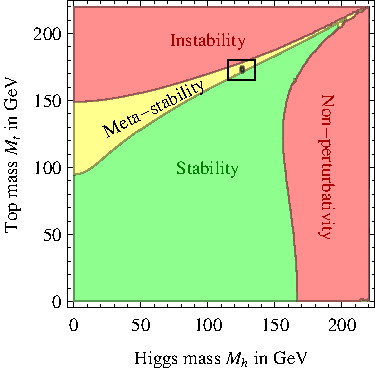
\includegraphics[width=0.45\textwidth]{figs/theory/SMstability.pdf}
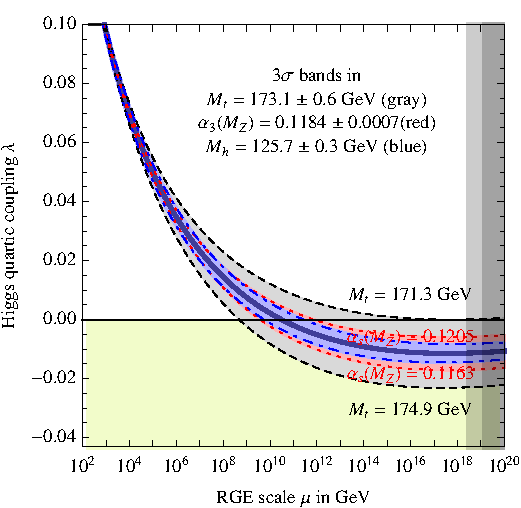
\includegraphics[width=0.45\textwidth]{figs/theory/runLambda.pdf}
\caption {
  RGE for the running of the SM parameter, $\lambda$ for the Higgs self-coupling term 
  with present values and uncertainty bands for $M_H$ and $M_t$ (left). The two-dimensional
  plot colored (right) shows regions for which the SM is stable, unstable, and metastable
  based on this RGE}

\label{figure:theory_stability}

\end{figure}


\section{Conclusion}

The Standard Model, despite its success in providing a unified description of fundamental
particles and interactions into single theory, has its flaws. These have been discussed in 
depth elsewhere, but include issues like the description of massive neutrinos, the failure
to include gravity, and the unnaturalness of large quantum corrections to Higgs parameters.
For these reasons, it seems the SM might be a lower energy approximation to a more fundamental
theory. The discovery of the Higgs boson at the LHC provided a stunning verification of one
of the fundamental aspects of the theory but at the same time offers new area to search for
glimpses of something grander. The production of samples of Higgs bosons
allows for a rich array of new tests of the Standard Model, which is now finally over-constrained by experiment. 
Searches for the $t\bar{t}H$ production, one category of which is the topic
of this thesis, provide tree-level access to a central parameter of the theory, the top Yukawa coupling,
as well as access a variety of Higgs decays, which will eventually provide a rigorous new 
test of the SM. 



%% \chapter[htoc-titlei][hhead-titlei]{htitlei}
%% -----------------------------------------------------------------------------
\chapter[The Large Hadron Collider][The Large Hadron Collider]{The Large Hadron Collider}
<<<<<<< HEAD
%test
Production of a sufficient number of high energy collisions to adequately explore
particle physics at the electro-weak scale required the development of one
of the most complex machines ever built, the Large Hadron Collider or LHC. This chapter
provides a very brief overview of the machine with particular focus on the 2012
dataset of proton-proton collisions it enabled. 
The technology involved in the development of the LHC and very breifly
touched upon in this chapter is an enormous achievement
it its own right and is documented in detail here \cite{1748-0221-3-08-S08001,Pettersson:291782,Linnecar:1176380}. 


\section{The Large Hadron Collider}

The LHC is the world's highest energy particle accellerator 
=======
\section{The Large Hadron Collider}

The Large Hadron Collider(LHC) is the world's highest energy particle accellerator 
>>>>>>> FETCH_HEAD
and is located 100m underneath the Franco-Swiss border at the European Organization
for Nuclear Research (CERN) in a 26.7 km tunnel. 

The LHC is a ciruclar 
machine capable of accelerating beams of protons and colliding them at center of mass 
energies up to $\sqrt{s} = 14 TeV$ at 4 collision sites around the ring, where 4 experiments
<<<<<<< HEAD
are housed (ATLAS\cite{ATLAS_detector}, CMS\cite{748-0221-3-08-S08004}, LHCb\cite{1748-0221-3-08-S08005}, and ALICE\cite{1748-0221-3-08-S08002)}. Figure \ref{figure:lhc_lhc} is a diagram
of the layout of the LHC and its experiments\cite{Team:40525}. The LHC also operates in a modes with beams of 
heavy ions. The LHC is composed of thousands of super-conducting Niobium-Titantium 
magnets, cooled to 2.7$^\circ$ C with liquid Helium, which steer and focus the 
particle beams, and a superconducting resonant-frequency (RF) cavity,which boosts the beam
to higher energies. 

% magnets
\begin{figure}[!t]
\centering 
\includegraphics[width=0.35\textwidth]{figs/lhc.pdf}
\caption{ Diagram of the Large Hadron collider and location of the 4 main experiments (ATLAS, CMS, LHCb, and ALICE). Around
  the ring. The diagram also shows the location of the SPS, the final booster ring the accelerator complex that accelerates
    the protons to 450 GeV before injection into the LHC. 
}
\label{figure:lhc_lhc}
\end{figure}



\subsection{The Accelerator Complex}

The accelerator complex is a progressive series of machines that progressively boost
the particle beams to their final beam energy and intenstiy.
=======
are housed (ATLAS, CMS, LHCb, and ALICE). The LHC also operates in a modes with beams of 
heavy ions. The LHC is composed of thousands of super-conducting Niobium-Titantium 
magnets, cooled to 2.7$^\circ$ degrees
% magnets


The technology involved in the development of the LHC is an enormous achievement
it its own right and is documented in detail here. 

\subsection{The Accelerator Complex}

The accelerator complex is a progressive series of machineswith the LHC as the final stage.
>>>>>>> FETCH_HEAD
Protons are obtained from hydrogen atoms and are accelerated to 50 MeV using the
Linac2, before being injected into the Proton-Synchrotron Booster (PSB). In
the PSB the protons are accelerated to energies of 1.4 GeV for injection
in to the Proton-Synchrotron (PS). The PS accelerates the protons to 25 GeV
and dumps bunches into the Super Proton Synchrotron (SPS), where they 
are accelerated to 450 GeV and finally dumped into the LHC. 

\subsection{Beam Parameters and Collisions} 

<<<<<<< HEAD
For the physics studied at the ATLAS experiment, the two most important parameters of
the collisions provided by the LHC are the center of mass energy and instantaneous luminosity.
High center of mass energies are necessary for the production
of new high mass particles, and because the consitutents of the actual collisions
are the partons of the proton, the CME of the collisions must in general
be much higher than the mass of the particles needed to be produced. The

\begin{figure}[!t]
\centering 
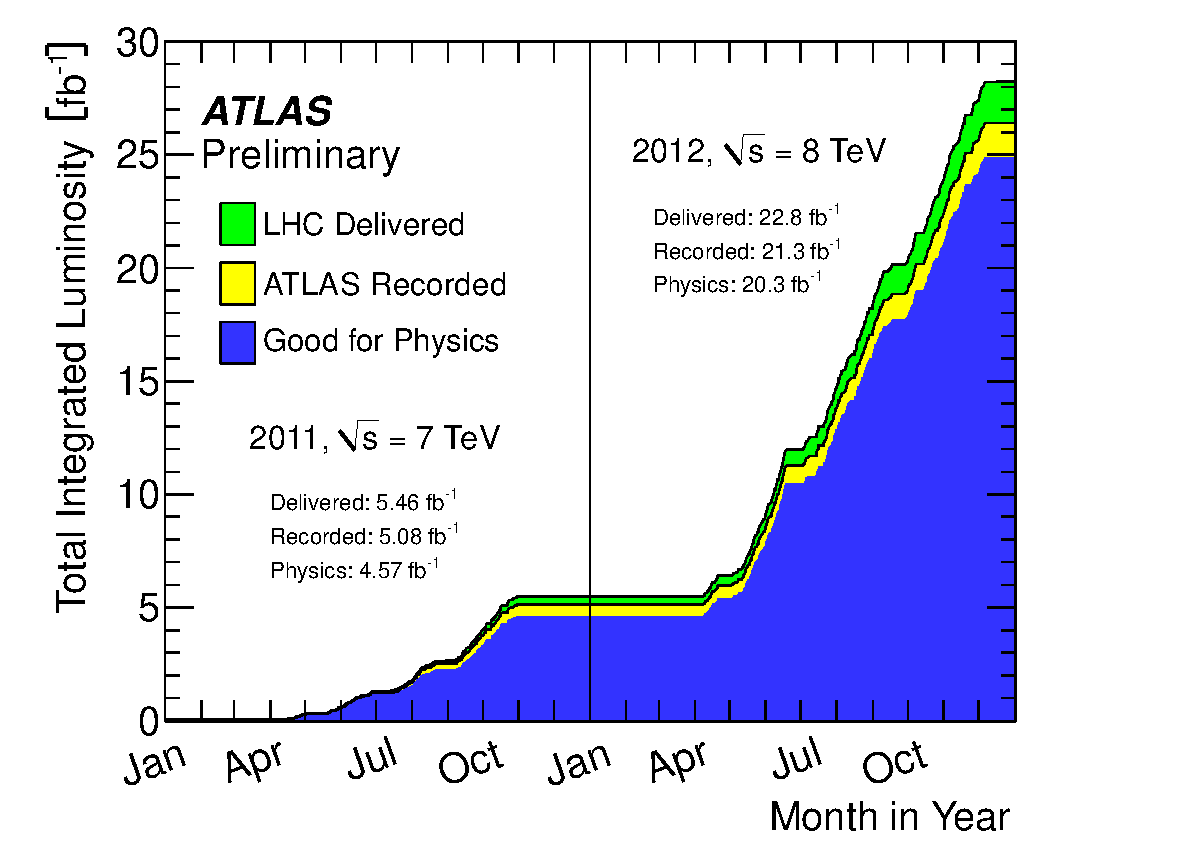
\includegraphics[width=0.35\textwidth]{figs/intlumivstime2011-2012DQ.pdf}
\caption{ Plot showing the accumulation of the integrated lumonisity delivered to the ATLAS experiment over 2011 and 2012. The rough size of the usable, physics ready dataset for 2012 is 20 $fb^-1$ and is the dataset used for the following analysis. 
}
\label{figure:lhc_lumi}
\end{figure}
The instantaneous luminosty of the collisions, \mathscr{L}, is a measure of the
collision rate. The integrated luminosity over time is a measure of the size
of the dataset and when multiplied by the cross-section of a particular process
gives the total number of expected events produced for that process.
Instantaneous luminosity depends on the number of colliding bunches of protons,
the intensity of those bunches, the revolution
frequency, and the nomralized transvserse spread of the beam in momentum and position
phase space, called the emmitance, and the transverse beam size. The LHC has the
option for colliding beams with 2808 bunches of protons, each with around $10^11$ protons,
at a rate of one bunch collision every 25 ns, or 40 MHz. These correspond
to a design luminosity of around $10^34$ cm$^{2}$ s$^-1$ or 10 nb$^-1$ s$^-1$
  
\section{The 2012 Dataset} 

The LHC successfully produced datasets for physics studies in 2010, 2011 and 2012. The 2012 
proton-proton dataset was delivered with collisions with a CME of 8 TeV with bunch collisions
every 50 ns and reached a total integrated luminosity of around ~20 fb$^-1$ \cite{Aad:2013ucp}.
Figure\ref{figure:lhc_lumi} shows the accumulation of this dataset over time. 
The full LHC design energy was never reached due to worries about faulty dipole
connections invovled in the unexpected quenching of the magnets in 2008. Despite doubling
the bunch spacing (thereby halving the bunch collision frequency), the lumonisty neared
the design lumonisty due to unexpected improvements in the transverse beam profile\cite{Carli:1424362}. This increased
the amout of pile-up, or number of collisions per bunch crossing and in general collision
events were busier due to these multiple interactions\cite{}. Figure \ref{figure:lhc_pileup} shows
the average number of interaction per bunch crossing for the 2011 and 2012 datasets. The 2012
dataset shows an average of 20-25 interactions. 

\begin{figure}[!t]
\centering 
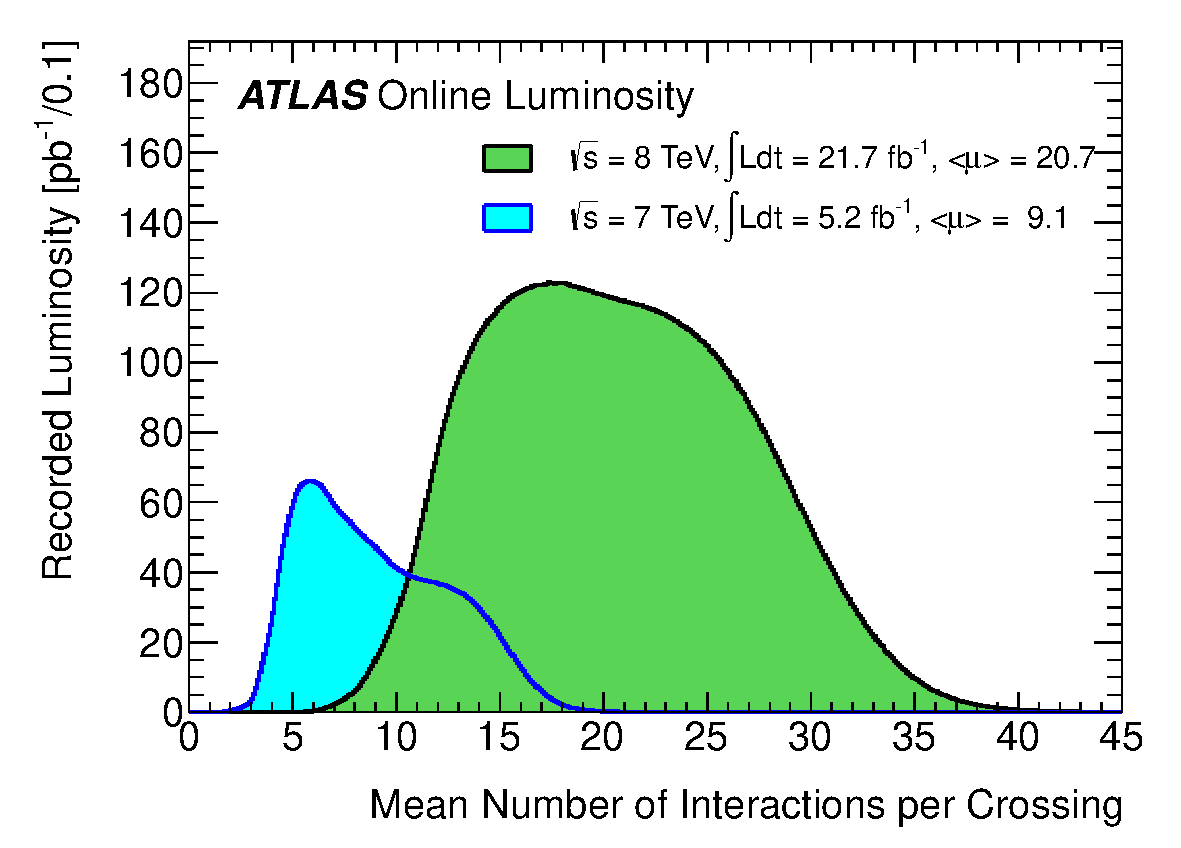
\includegraphics[width=0.35\textwidth]{figs/mu_2011_2012-dec.pdf}
\caption{ The average number of interactions per bunch-crossing for the 2012 and 2011 LHC proton-proton dataset. Most of these interactions are unintersting but leave energetic signatures in particle detectors called pile-up which interfere with measurements}\label{figure:lhc_pileup}

=======



\section{The 2012 Dataset} 
>>>>>>> FETCH_HEAD

\chapter[Electrons][Electrons]{Electrons}
\label{chapter:electron} 

High energy electron signatures are important elements of seaches and measurements at hadron colliders, because they signal the presence of important electo-weak processes in the event. Requiring well-identified electrons in collision events quickly suppresses the overwhelming rate of strong-force mediated scattering and allows for the collection of a manageably-sized dataset with intersting physics for study. For this reason, electron signatures form one of the two pillars of the HLT trigger at ATLAS, as discussed in Chapter~\ref{chatper:lhc} and rigorous electron identification is an important peice of many ATLAS analyses. This section summarizes the development of ATLAS electron identification for the high luminosity 2011 and 2012 datasets and discusses the techqniues invovled in measuring the electron identification efficiency. 

\section{Identification of Electrons at ATLAS}

%picutres and example figures

Electron reconstruction is discussed briefly in Chapter~\ref{chatper:lhc} and, in depth here~\cite{}. The result of electron reconstruction is called an electron candidate, which is comprised of a narrow calorimeter energy cluster with $|\eta| < 2.47$ and inner detector track that matches loosely in $\eta$ and $\phi$. If the electron has $|\eta| < 2.01$, the the inner detector track is fiducial to the TRT has has the possibility of having high-threshold hits, indicative of transition radiation (TR). Electron cluster recontruction is extremely efficient. The track-matching requirement is less efficient, because the presence of hard bremsstrahlung may in certain cases cause the electron cluster and emitted photon cluster to have a wide separation in the calorimeter\cite{}. 

Objects that are not isolated electrons are often reconstructed as electrons, as the reconstruction requirements are quite loose. Objects that often `fake' isolated electrons are light quark and gluon jets, heavy flavor jets that include real decays to electrons and converted photons. Light quark and gluon jets fragment into a number of collimated hadronic particles. In rare cases, the jet may fragment most of its energy into a single charged pion, which showers early in the EM calorimeter. In other rare cases, the jet may fragment mostly into a neutral pion, which subsequently decays into a pair of photons. If one of these photons converts, a track will point to the EM energy cluster. These cases would result in a reconstructed electron candidate. Although the probability for this to happen is small, the enormous jet production rate means that it is a significant background. In general, light quark and gluon jet `fakes' have larger transverse shower profiles and more energy leakage into the hadronic calorimeter. For the neutral pion case, there are generally two separated showers for lower energy decays. For both cases, there are often other particle signatures nearby.  
On the other hand, heavy-flavor jet decays and photon conversions contain real electrons. However, heavy flavor decays also involve the production of additional hadronic particles within the jet and both photon conversion and heavy flavor decays involved secondary vertices displaced from the primary interaction point. 

In order to distinguish these fake signatures from real isolated electrons, electron identification algorithms use a number of reconstructed variables describing the electron shower in the detector and the electron track. The details of the calculated variables can be found here~\cite{}. In general, the calorimeter variables take advantage of the narrowness of isolated electron shower in the transverse plane and lack of energy deposition in the hadronic calorimeter. The transverse variables include measurements of the shower width in both layer 2 and the strips, where more refined measurements are possible. In fact, the strips were designed to separate single photon and eletron showers from multiple showers from neutral pion decays, shown in Figure \ref{}. The shower width variables are generally measured mostly in $\eta$ as bremstrahlung tends to smear the electron energy in $\phi$. Electron tracks are required to have an adequate number of hits in the Pixel Detector, SCT and TRT. These hit requirements, especially the b-layer requirment suppress electron conversions which occur in the detector material. Track-cluster matching and geometric impact parameter variables require ID tracks to match the calorimeter energy well and to arise from the primary interaction point, respectively. Electrons with tracks explictly associated with a conversion vertex may be rejected. Finally, the high threshold fraction of hits on the track, made by transition radiation is an uncorrelated discrimator of pion and electron tracks.


Electron identification algorithms make selections in 9 bins of $|\eta|$, [0.10, 0.60, 0.80, 1.10. 1.37, 1.52, 1.81, 2.01, 2.37, 2.47] and bins of \pt, [7, 10, 15, 20, 30, 40, 50, 60, 70, 80$+$]. The $|\eta|$ binning changes with the calorimeter geometry, which in turn affect the shower shape distributions. The shape of most of the identification variable distributions, tracking and calorimeter, are \pt\ dependent.  


\begin{figure}

\end{figure}

\subsection{Pile-up and Electron identifiation}

\subsection{2011 Menu}

Electron identification in 2011 was accomplished through rectangular cuts on the identification variables at 3 operating points: Loose, Medium and Tight. The medium operating point was used online as the primary electron trigger. At the bbeginning of the 2011 run, the 3 operating points possessed the same cuts, but tighter operating points had cuts on more variables. The Loose operating point only cut on shower shape variables in layer 2 and hadronic leakage, the medium operating point added cuts on shower width variables in the strips, and tight added TR cuts, strict-track cluster matching, conversion rejection and a b-layer requirement. This menu, called the `IsEM' menu, was the first fully data-optmized cut menu for electrons. 

The demands of increasing luminostiy demanded a tightening of the medium operating point midway through the data-taking, in order to maintain a EF trigger rate of around 20-25 Hz on the primary electron trigger. To accomplish this, variables cut on at the tight operating point were added to the medium operating point, and the entire set of cuts was optimized to provide the targeted fake rejection and reduction in the rates at the highest possible efficiency. The same procedure was applied to the loose operating point, where the target was to provide efficiencies of 95\% and the highest possible fake rejection. The re-inventing of the menu in this way allowed for not only better performance, due to the inclusion of more variable, but a more stable tightening of the backgrounds from loose to medium to tight, where the same backgrounds types were targeted at each level. The new menu was called the `IsEM$++$' menu and the operating points were renamed `Loose$++$', `Medium$++$' and `Tight$++$'. Figure \ref{} shows the comparison of the operating points for the new menu and old menu.

\subsection{2012 Menu and Pile-up}

Improvements in the running conditions for 2012, in particular narrowing the transverse beam emittance and size, resulted in large increase in number of proton-proton interactions during every 50 ns bunch crossing. In 2011 the average number of reconstructed primary vertices in each event, an indicator of the number of interaction per bunch crossing, was around 7, while in 2012 the average grew to 25. Some events during 2012 running had 40 reconstructed primary vertices.

The increase in energy in the calorimeters from these additional collisions, called pile-up, caused a worsening of the resolution of electron identification variables, particularly the shower shapes and hadronic leakage.The presumed cause was the increase in the number of showers of low energy hadronic particles nearby electrons.  Figure~\ref{} shows an example distribution, the hadronic leakage under different pile-up conditions. The distributions shows a clear widening which results in a loss of efficiency. 

In order to combat this loss, the `IsEM$++$' menu was once again optimized to have a flatter efficiency profile as a function of the amount of pile-up in the event with similar perfromance to the 2011 menu. The strategy for this menu was to loosen selections on variables sensitive to pile-up energy. It was expected and confirmed that relying more on the strip variables for the shower shape selection and the energy in layer 3 of the EM calorimeter for the hadronic leakage, would use a smaller volume of the calorimeter and thus be less sensitive to additional energy in the neighborhood of the electron. The strategy is outlined pictorally in Figure~\ref{}.  

The efficiency of the 2011 operating points compared to the 2012 operating points is shown in Figure~\ref{}, demonstrating a clear improvement in effiency of the selections for higher pile-up conditions. Finally, the 2012 primary electron trigger to include highly efficient tracking isolation criteria in order to 

\subsection{Electron Likelihood}

A natural step forward for the electron identification is the use of multi-variate algorithms. Multi-variate identification algorithms use many identification variables at once in a multi-dimensional space and judge where signals and backgrounds are found in that space to make decisions

For the case of electron identification, it was found that using a likelihood function, trained with electron identification variables, provided clear perfmance gains with respect to rectangular cuts, while also providing stable and easily understandable results. The likelihood scores each electron based on how signal-like or background  it is for each individual indentification variable and then multiplies these identification variables together into a final score. Figure~\ref{} shows 

XXX equations?


There are many advantageous to a likelihood based approach. First, variables that show signficant shape differences between real and fake electrons but do not have a clear cut point can still be used in a likelihood. Second, the likeihood score takes into account the entire shape of the distribution and not simply an efficiency and fake rejection at a single cut point. Finally, the final cut on the likelihood output score.

The likelihood menu for ATLAS was developed at the end of the 2012 Run to be used on advanced 2012 analyses. The menu uses similar variables to the cut-based menus but adds a few additional variables, including a measurement of the amount of energy the electron track lost as it traversed the ID. The likeihood menu makes cuts on the likelihood output score at 4 different operating points with the same binning as the cut menu but tunes the cuts based on the amount of pile-up in the event. The likelihood menu greatly outperforms the rejection of the `IsEM$++$' menu for similar efficiencies. Figure XXX shows. The likelihood menu, specificaly the \textsc{verytight} operating point, is used in the \tth\ analysis.  

\section{Measurement of Electron Identification Efficiency at ATLAS}

Precise measurements of the electron identification efficiency are important pieces of many ATLAS analyses, including the \tth\ multi-leptons analysis. For analyses with low \pt\ leptons, systematic uncertainties on the electron identification efficency can be some of the largest sysetmatic effects. The methods used to measure the electron identification efficiency are described in depth here \cite{}. 

Electron identifications efficiencies are measured using a method called tag-and-probe for $J/\Psi$ and $Z$ boson decays to electrons. One object from the decay is tagged, while the other electrons is left unidentified. Reasonable confidence that the second object, thought not identified, is an electron based on the kinematic properties of the event, specifically the di-electron invariant mass is near the $Z$ of $J/\Psi$ pole. The tag-and-probe method leaves a sample of unidentified and unbiased probes, where the efficiency can be measured.

As opposed to muons, contamination from fake electron make the tag-and-probe method difficult. This is especially true for electrons in with \pt\ of 10-20 GeV. The energy scale of $Z$ and $J/\Psi$ decays disfavor electrons of this momentum, but low energy electrons are important in a number of Higgs searches. Backgrounds from fake electrons are subtracted using fits to the $Z$ and $J/\Psi$ invariant mass distributions. For $Z$ electrons, fits to the electron isolation distribution are also used. The final efficiencies reported are the result of statistical fit among all methods. The uncertainties are at low momenta are around $\sim$ 5\% and are dominated by systematics effects from large background subtractions. They are less than 1\% at high momenta and dominated by tag-and-probe selection effects.

\subsection{Issues}

For the measurement of the 2012 electron identification efficiencies, an inconsistency between the isolation-based background subtraction method and   

%% \chapter[htoc-titlei][hhead-titlei]{htitlei}
%% -----------------------------------------------------------------------------
\chapter[Search for the TTH Decay in the Multilepton Channel][Search for the TTH Decay in the Multilepton Channel]{Search for the TTH Decay in the Multilepton Channel}
\label{chapter:analysis} 
This chapter provides an overivew of the the set of analyses searching for the Standard Model
(SM) production of the Higgs boson in association with top quarks in
multi-lepton final states with multiple jets (including b-quark tagged jets).
Searches in $t\bar{t}H$ final states with 2 same-charge, 3 and 4 light leptons
($e, \mu$) are discussed in depth. These final states target specifically Higgs
decays to vector bosons, $H\rightarrow W^{\pm}W^{\pm}$ and $H\rightarrow
Z^{\pm}Z^{\pm}$ and form a complement to searches for $t\bar{t}H$ production in
final states targeting the $H\rightarrow b\bar{b}$ \cite{Aad:2014lma},
      $H\rightarrow\gamma\gamma$\cite{ATLAS-CONF-2014-011}, and $H\rightarrow\tau\tau$ decay modes.


Based on SM production cross-sections, observation lies just outside the sensitivity
of the Run I dataset, even when combining all searches. The analyses provide an opportunity to 
constrain for the first time the \tth production mode with limits reasonably close to the
actual production rate. As such the analysis is optimized to overall sensitivty to the 
\tth production rather than individual decay modes, which would be more useful for
constraining Higgs couplings. 


Detailed description of the event and objection section are provided in Chapter \ref{chapter:selection},
background modelling in Chapter \ref{chapter:background}, the effect of syetmatic errors and the 
statistical analysis in Chapter \ref{chapter:systematics} and final results in Chapter \ref{chapter:results}.


\section{Signal Characteristics} 
\tth can be observed in a number of different final states realted to the
the Higgs boson and the top quark decay modes.

Three Higgs boson decays are relevant for this analysis: \WW,
\twotau and \ZZ. The top and anti-top quarks decay  in
\Wb. Each \W boson decays either 
leptonically (l=$e^\pm$, $\mu^\pm$,$\tau^\pm$) with missing energy or hadronically. 
Table \ref{ana:table_decay} provides the fractional contribution of the main 
Higgs decay modes at the generator level to \tth search channels. These
numbers will be modified by lepton acceptances. 

\begin{table}[htbp]
  \begin{center} 
    \caption{Contributions of the main Higgs decay modes to the 3 multilepton
      \tth signatures at generation level.
      }\label{ana:table_decay} 
      \begin{tabular}{l|c|c|c} 
      \hline\hline
  Signature & $H \rightarrow WW$  & $H\rightarrow \tau\tau$  & $H \rightarrow
  ZZ$  \\\hline
  Same-sign &  $100\%$ & -- & -- \\
  3 leptons  &  $71\%$ & $20\%$ & $9\%$ \\
  4 leptons  &  $53\%$ & $30\%$ & $17\%$  \\
     \hline
    \end{tabular}
  \end{center}
\end{table}


All modes are generally dominated by the $WW$ signature, though the 3l and 4l
channnels possess some contribution from the$\tau\tau$ and $ZZ$ decays. 


The signal is expected to be characterized by the presence of 2 b-quark jets from
the top quark decays, leptons from vector boson and tau decays,
a high jet multiplicity, and missing energy. In general, the number of leptons is anti-correlated 
with the number of jets, since a vector boson can either decay leptonically 
or hadronically. For \hww, the light quark multiplicity, $N_q$, and the
number of leptons, $N_l$, follow this relation: $2N_l+N_q+N_b=10$.

\begin{itemize}
\item In the same-sign channel, the \tth final state contains 6 quarks. These events
are then characterised by a large jet multiplicity.

\item In the 3 lepton channel, the \tth final state contains 4 quarks from the hard scatter.

\item In the 4 lepton channel, the \tth final state contains a small number of light
quarks, 0 (\hww case), 2 or 4 (\hzz case).


\end{itemize} 

\section{Background Overview}

Background processes can be sorted into two categories:

\begin{itemize}

\item Events with a non prompt or a fake lepton selected as prompt
  lepton. These processes cannot lead to a final state compatible with the
  signal signature without a misreconstructed object. This category includes
  events with a prompt lepton but with misreconstructed charge\footnote{Charge mis-identification is almost exlusively a phenomenon of electrons at our energy scales. While it is
  is possible for both electrons and muons to have an extremely straight track, whose direction of curvature is difficult to measure, the happens only at extremely high momentum. 
  Electrons on the other hand may interact with the detector material, resulting in bremmstrahlumg. The bremstrahlung photon may subsequently convert resulting in 2 additional
  tracks near the original electron. This process, called a trident process, may cause a mismatching of the electron cluster with the original electron track and thus
  a charge-mis identification and happens also at low energies}and events
  with jets that "fake" leptons.  These processes are rejected with tight object isolation and identification criteria, requiring a large jet multiplicty, and veto-ing events
  consistent with a leptonically decaying Z boson. 

  The main backgrounds of this sort are: \ttbar and \zj.
  Data-driven techniques are used to control some of these processes.
  Their importance varies depending on the channel.

\item Events which can lead to the same final state as the signal (irreducible
  backgrounds).
 The main background of this category are: \ttV, \WZ, and \ZZ.
 They are modeled using the Monte Carlo simulations. In general,
 these backgrounds are combatted with jet and b-tagged jet requirements. 
 Although the jet multiplicty of \ttV is high, the multiplicity of \tth 
 events is still higher. 

\end{itemize}


\section{Analysis Strategy} 


ADD SOMETHING HERE FOR HOW TO CALCULATE A CROSS-SECTION

The analysis search is conducted in 3 channels, based on counting of fully identified
leptons: 2 SS leptons, 3 leptons,and 4 leptons. The lepton counting occurs before additional object cuts are made in each individual 
channel to ensure orthoganility. The division into lepton channels rather than channels targeting specific decay modes
allows channels with different sensitivities to considered separately. We further divide the 2l SS into sub channels
based on the number of jets and flavor of the leptons and the 4l channel into subchannels enriched and depleted in OS leptons arrising from Z decays. 

The channels are fed into a posson model 




\chapter[Dataset and Simulation][Dataset and Simulation]{Dataset and Simulation}
\label{chapter:data} 
\section{Data}

\subsection{The 2012 Dataset} 

The LHC successfully produced datasets for physics studies in 2010, 2011 and 2012. The 2012 
proton-proton dataset was delivered with collisions with a CME of 8 TeV with bunch collisions
every 50 ns and reached a total integrated luminosity of around ~20 fb$^-1$ \cite{Aad:2013ucp}.
Figure\ref{figure:data_lumi} shows the accumulation of this dataset over time. 
Despite doubling the bunch spacing (thereby halving the bunch collision frequency), the lumonisty neared
the design lumonisty due to unexpected improvements in the transverse beam profile\cite{Carli:1424362}. This increased
the amout of pile-up, or number of collisions per bunch crossing and in general collision
events were busier due to these multiple interactions. Figure \ref{figure:data_pileup} shows
the average number of interaction per bunch crossing for the 2011 and 2012 datasets. The 2012
dataset shows an average of 20-25 interactions. 
\begin{figure}[!t]
\centering 
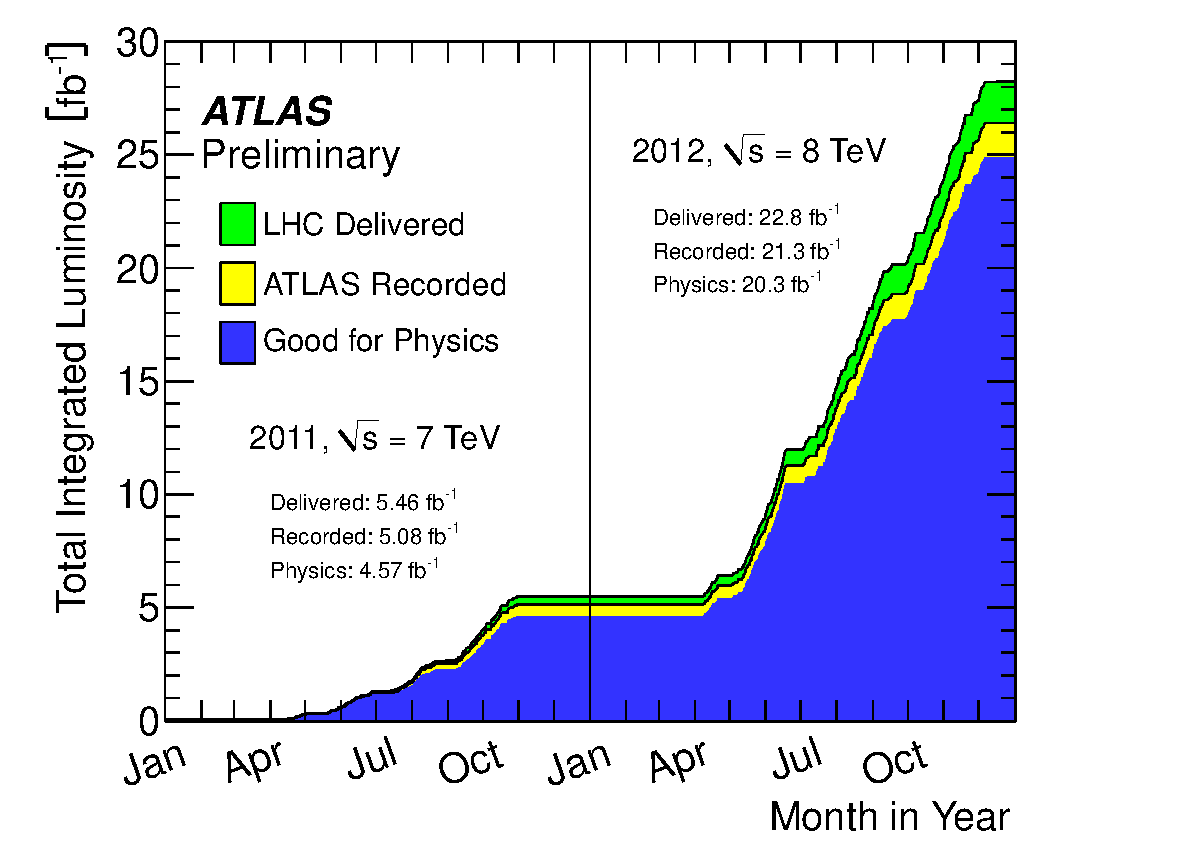
\includegraphics[width=0.60\textwidth]{figs/intlumivstime2011-2012DQ.pdf}
\caption{ Plot showing the accumulation of the integrated lumonisity delivered to the ATLAS experiment over 2011 and 2012. The rough size of the usable, physics ready dataset for 2012 is 20 $fb^-1$ and is the dataset used for the following analysis. 
}
\label{figure:data_lumi}
\end{figure}


\begin{figure}[!t]
\centering 
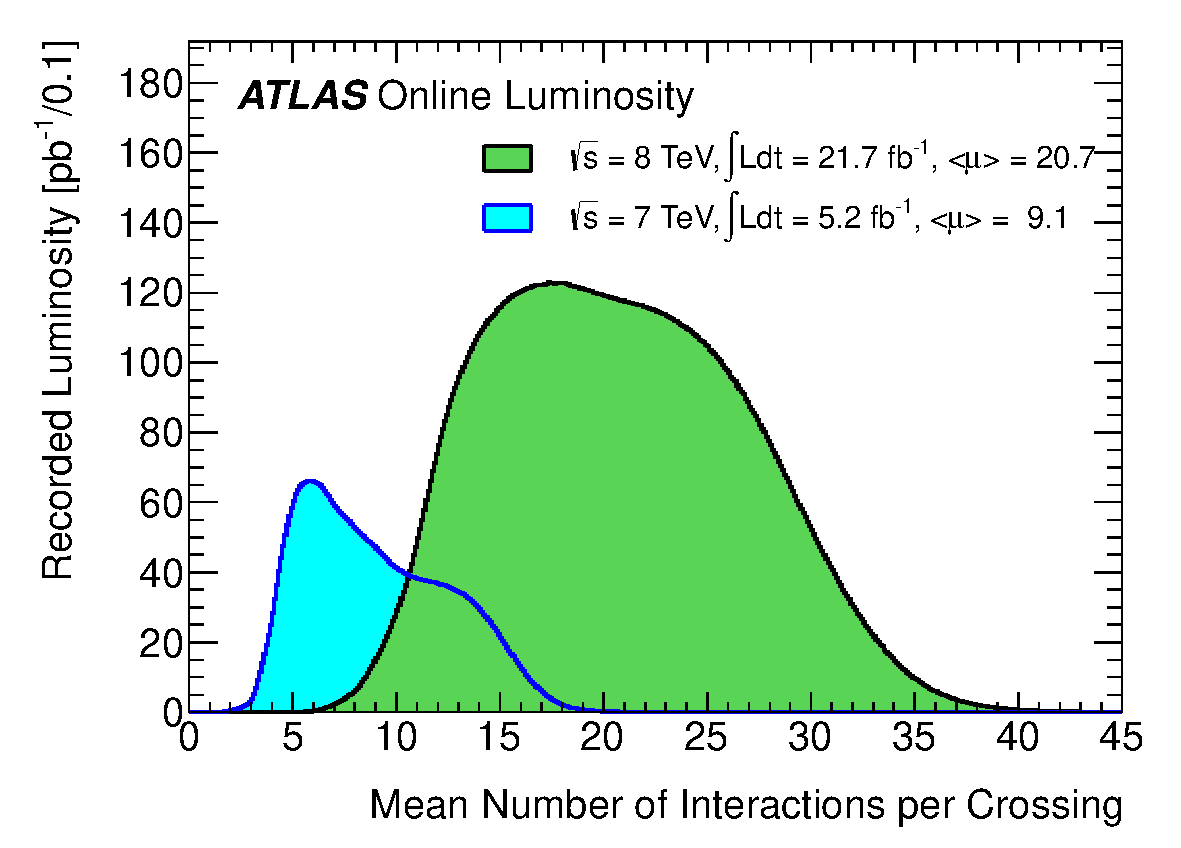
\includegraphics[width=0.60\textwidth]{figs/mu_2011_2012-dec.pdf}
\caption{ The average number of interactions per bunch-crossing for the 2012 and 2011 LHC proton-proton dataset. Most of these interactions are unintersting but leave energetic signatures in particle detectors called pile-up which interfere with measurements}\label{figure:data_pileup}
\end{figure} 

The \tth analysis uses the entire 2012 ATLAS dataset, collected
from April to December. The size of the dataset corresponds to 20.3 \ifb, after passing data quality
requirements, ensuring the proper operation of the tracking, calorimeter and muon subsystems.  

The datasets used in the analysis were collected with the primary electron
(EF\_e24vhi\_medium1 || EF\_e60\_medium1) and muon triggers (
    EF\_24i\_tight || EF\_36\_tight). The electron triggers require a electron
with at least 25 \gev\ of calorimeter energy, passing the medium identification
requirement and loose tracking isolation.  Above 60\gev, the isolation
requirement is dropped and the identification is loosened slightly. Similarly,
            the muon trigger requires a good inner detector track and matching
            hits in the muon spectrometer, as well as loose tracking isolation,
            which also is dropped about 36 \gev\.  The data sample must contain
            either a primary muon or primary electron trigger. 

\section{Simulation}

Simulation samples based on are used to determine the 
overall event selection acceptance and efficiency and for investigations not directly invovled
in the final result The simulated samples are created using parton distribution function (PDF) and
model using Monte Carlo (MC) techniques the hard parton scatter, underlying event activity and parton showering and hadronization. 
The samples are then passed through a full ATLAS detector simulation\cite{Aad:2010ah} based on  GEANT4 \cite{Agostinelli:2002hh}.
Small corrections are then applied to the overall efficiencies to re-scale object identification efficiencies,
      energy scales, and the pile-up, discussed in depth later.  

\subsection{Signal Simulation}


The \ttbar$H$ production is modelled using matrix elements obtained from the HELAC-Oneloop package~\cite{Helac} that corresponds to the next-to-leading order (NLO) QCD accuracy. POWHEG BOX~\cite{powheg,powbox1,powbox2} serves as an interface to the parton shower Monte Carlo programs. The samples created using this approach are referred to as {\textsc PowHel} samples. {\textsc CT10NLO} PDF sets are used and the factorisation ($\mu_{\rm F}$) and renormalization ($\mu_{\rm R}$) scales are set to $\mu_{0} = \mu_{\rm F} = \mu_{\rm R} = m_{t}+\mH/2$. Pile-up and the underlying events are simulated by {\textsc Pythia} 8.1~\cite{PythiaManual8} with the {\textsc CTEQ61L} set of parton distribution functions and AU2 underlying event tune. The Higgs boson mass is set to $125\gev$ and the Top quark mass is set to $172.5\gev$.\\
The signal Monte Carlo samples are summarized in Table~\ref{table:data_mcsignal}.
These large samples are generated with inclusive Higgs boson decays, with
branching fractions set to the LHC Higgs Cross Section Working Group (Yellow Report)
recommendation for $m_H = 125$ GeV \cite{Heinemeyer:2013tqa}.  The inclusive cross section (129.3
fb at $m_H = 125$ GeV) is also obtained from the Yellow Report \cite{Heinemeyer:2013tqa}.



\begin{table}
\begin{center} 
    \caption{Monte Carlo samples used for signal description.}\label{table:data_mcsignal}
   \begin{tabular}{l|c|c|c|c} 

      \hline\hline
       Process & Generator & Cross- & $\mathcal{L}$ [\ifb]  & Detector \\ 
               &           & section [fb] &            &  simulation \\
\hline
 ttH$\rightarrow$allhad+H & PowHel+Pythia8 & 59.09 & 2146.5 & Full \\
 ttH$\rightarrow$ljets+H & PowHel+Pythia8 & 56.63 & 2238.9 & Full \\
 ttH$\rightarrow$ll+H & PowHel+Pythia8 & 13.58 & 9332.0 & Full \\
\hline\hline
    \end{tabular}
  \end{center}
\end{table}


\subsection{Background Simulation}

The background simulations used for this analysis are listed in
Table~\ref{table:data_MCbackground}.  In general, the Alpgen\cite{Mangano:2002ea}, MadGraph\cite{Maltoni:2002qb}, and AcerMC\cite{Kersevan:2004yg} samples use the CTEQ6L1\cite{Nadolsky:2008zw}
parton distribution function, while the Powheg\cite{Frixione:2007vw}, Sherpa\cite{Gleisberg:2008ta}, are generated with the CT10 PDF.  The exception is the MadGraph $t\bar t t \bar t$ sample, which is generated with the
MSTW2008 PDF\cite{Martin:2009iq}. The highest order calculations available are used for cross
sections.  


\begin{table}
\begin{center} 
    \caption{Monte Carlo samples used for background
      description.  Unless otherwise specified MadGraph samples use Pythia 6
      for showering and Alpgen samples use Herwig+Jimmy.}\label{table:data_MCbackground}

\begin{tabular}{l|l|c}
      \hline\hline
       Process & Generator   & Detector \\ 
               &             &  simulation \\
      \hline\hline
\ttW,\ttZ & MadGraph & Full \\
\tZ       & MadGraph & AF2 \\
$t\bar t t \bar t$ & MadGraph & Full \\
\ttWW & Madgraph+Pythia8  & AF2 \\
\ttbar & Powheg+Pythia6  & Full/AF2 \\
single top tchan & AcerMC+Pythia6& Full \\
single top schan$\rightarrow$l   & Powheg+Pythia6 & Full \\
single top $W^{\pm}t$ & Powheg+Pythia6 & Full \\
W$\gamma$*& MadGraph & Full \\
W$\gamma$+4p & Alpgen & Full \\
\WW & Sherpa &  Full \\
\WZ & Sherpa &  Full \\
Same-sign WW & Madgraph+Pythia8 & AF2 \\
ZZ$\rightarrow$ & Powheg+Pythia8,gg2ZZ+Herwig & Full \\
Z$\gamma$*  & Sherpa  & Full \\
Z+jets & Sherpa & Full \\
ggF\_H(125) & Powheg+Pythia8 & Full \\
\end{tabular}
\end{center}
\end{table}



\chapter[Object and Event Selection][Object and Event Selection]{Object and Event Selection}
\label{chapter:selection}

MAKE COOL PLOT FOR THIS

The analysis is divided into 3 signal regions based
on lepton counting: 2 same-sign leptons, 3 leptons and 4 leptons. The lepton
counting occurs for fully identified leptons with full overlap removal with
transverse momenta over 10 \gev\ to ensure orthogonality. Lepton selections are tightened
afterward within each region.

The cuts for each signal region are provided in Table \ref{table:selection} and the object selections are detailed in the
following selections. The selections are based on optimizations of the region sensitivity
performed using MC (event for data driven backgrounds) and ad-hoc values for normalization systematic uncertainties\footnote{the sensitivity was approximated using the $\frac{s}{\sqrt{b + \Delta b}}$ formula. The systematic errors considered were 20\$ for \ttV and VV and 30\% for fakes. These ended up being close the final systematic errors assessed in Chapter~\ref{chapter:systematics}. The objects of optimization were the lepton momenta, identification operating points, isolation and event kinmeatic variables} 
All signal regions are comprised of three basic requirements: the presence of b-tagged
jets, the presence of additional light jets, and a veto of same flavor opposite sign leptons with an
invariant mass within the Z window. Additional requirements on the invariant mass of the leptons, the missing transverse energy
in the event, and the total object energy ($\rm H_{T}$) proved to have negligible additional benefit at our level of 
statistics.

\begin{table}[htbp]
  \begin{center} 
    \caption{Selections in the 2$\ell$ SS, 3$\ell$ and 4$\ell$ Signal Regions}
      \label{table:selection}
   {\small
    \begin{tabular}{|l|c|c|c|} 
  
  \hline 
  Signal Region   & 2$\ell$ SS & 3$\ell$  & 4$\ell$ \\\hline\hline
  Trigger Matched Lepton   & Yes & Yes    & Yes \\ \hline
  N$_{l}$\footnote{lepton counting is for \pt $=$ 10 GeV leptons, based on the standard criteria outlined in the sections that follow}& $=$2 &  $=$3       & $=$4 \\\hline
  Lepton Charge Sum & $+$2 or $-$2     & $+$1 or $-$1 & 0 \\ \hline
  Lepton Momentum (GeV)\footnote{lepton (0,1,2,3) are \pt ordered, with the exception of the 3$\ell$ case} & \pt$_0>$ 25   &  \pt$_0>$ 10 & \pt$_0>$ 25   \\
  & \pt$_1 >$ 20 &  \pt$_{1,2}>$25,20 & \pt$_1>$ 20 \\
  &                   &                          &  \pt$_{2,3}>$ 10 \\\hline
  Jet Counting    & N$_{b}\geq 1$, N$_{Jet} =$  4 & N$_{b}\geq 1$, N$_{Jet} \geq$ 4 & N$_{b}\geq 1$, N$_{Jet} \geq$ 2   \\
                  &                               &        or N$_{b}\geq 2$, N$_{Jet} =$ 3         &                                   \\\hline
  Mass Variables (GeV) & $|M_{ee} - M_{Z}| <$ 10  &  $|M_{SFOS}-M_Z| <$ 10  &  $M_{SFOS} >$ 10   \\
  &   &     & $150 <M_{4\ell} <500$    \\
  &   &     & $|M_{SFOS}-M_Z| <$ 10     \\\hline
  Sub-channels     & 2 (N$_{Jet}=4$, N$_{Jet}\geq$ 5) &  none  &  2 (No SFOS leps,    \\
  &  x 3(ee,e$\mu$,$\mu\mu$)  &     & SFOS leps)    \\\hline
    \end{tabular}} 
  \end{center}
\end{table}



\section{2$\ell$ Same-Charge Signal Region}

The 2 lepton same-sign signal region (2$\ell$ SS) requires two leptons of similar charge. The signal is symmetric in charge but
the background from opposite-sign \ttbar\ di-lepton production would be overwhelming. Requiring
only two leptons allows the extra 2 W bosons in the event to decay hadronically, resulting in on average 4 additional
light jets plus 2 additional b-quark jets from the top decays. 

We require a leading lepton with transverse momentum of at least 25 GeV that matches to a
trigger and a sub-leading lepton of at least 20 GeV, a b-tagged jet, and at least 4 jets in
total.  

In order to suppress non-prompt backgrounds, the lepton isolation criteria for tracking and 
calorimeter are tightened from less than 10\% of the lepton momentum to 5\%. To suppress
charge mis-identification, the electron is required to be extremely central ($|\eta| < 1.37$) 
to avoid the material-rich regions of the detector. Additionally, $ee$ events with a 
lepton pair invariant mass within 10 GeV of the Z pole are removed. To maintain orthogonality with the $\tau$ analyses, events with fully identified
taus are vetoed.

For the statistical combination the channel is divided into 6 sub-channels:
2 jets counting bins (N$_{Jet}$ $=$ 4, N$_{Jet}$ $\geq$ 5) x 3 lepton flavor bins (ee,$\mu\mu$,e$\mu$). 


\section{3$\ell$ Signal Region}

The 3 lepton channel requires 3 leptons, whose summed charge is either
$-$1 or $+$1. The leptons are ordered in this way:

\begin{itemize}
\item \textbf{lep0:} the lepton that is opposite in charge to the other two leptons
\item \textbf{lep1:} the lepton that is closer in $\Delta R$ to lep0
\item \textbf{lep2:} the lepton that is farther in $\Delta R$ from lep1
\end{itemize}

Since events with a fake lepton arise exclusively from opposite sign di-lepton processes, \ttbar\ and Z+jets, where additional jets are 
mis-identified as the third lepton, lep0 is never the fake lepton. As a result, the transverse momentum 
requirement of lep0 ($> 10$ GeV) is lower that the other two, $>$ 20 GeV.  One lepton must
must match a trigger and have $p_T >$ 25 GeV. 

The 3$\ell$ channel further requires at least one b-tagged jets and at least 4 jets in total, or two b-tagged jets and exactly 3 jets in 
total. Additionally, to suppress \WZ and \zj events, events with same-flavor opposite sign pairs
within 10 GeV of the $Z$ pole are vetoed.

Additional cuts, including a di-lepton mass cut, and splittings were investigated but low statistics proved to wash out any advantages.
The di-lepton mass cut will be a useful descriminant in future analyses since the spin statistics of Higgs decay in $W$ bosons often
causes the two emitted opposite-sign leptons to point in the same direction, resulting in a small measured invariant mass. 

\section{4$\ell$ Signal Region}

In the four lepton signal region, selected events must have exactly four leptons with a total charge of zero. 
At least one lepton must be matched to one of the applied single lepton trigger and have a transverse momentum above 25 GeV. 
The leading and sub-leading leptons are required to have transverse momentum of 25 and 15 GeV respectively. 
In order to suppress background contributions from low-mass resonances and Drell-Yan radiation, all opposite-sign-same-flavor (OS-SF) lepton pairs are required to have a dilepton invariant mass of at least 10 GeV. 

The four-lepton invariant mass is required to be between 100 and 500 GeV. 
This choice of mass window suppresses background from the on-shell $Z\to4\ell$ peak and exploits the high-mass differences between the signal and the dominant \ttZ background. 
Events containing an OS-SF lepton pair within 10 GeV of the Z boson mass are discarded. 
This Z-veto procedure greatly reduces background contributions from \ZZ and\ttZ. 
Finally, selected events are required to have at least two jets, at least one of which must be tagged as a b-quark jet.  

The contribution from \ttZ comprises approximately 75\% of the total background in the inclusive signal region. 
A signal region categorization which factorizes \ttZ from the remaining backgrounds is thus beneficial. 
The signal region is accordingly divided into two categories based on the presence of OS-SF lepton pairs in the final state. 

\section{Electron Selection}

The electrons are reconstructed by a standard algorithm of the
experiment~\cite{ATLAS-CONF-2014-032} and the electron cluster is required to be fiducial 
to the barrel or endcap calorimeters: $|\eta_{cluster}| < $ 2.47. Electrons
in the transition region, $1.37 < |\eta_{cluster}| < 1.52$, are vetoed.
Electrons must have \pt$>$10 GeV and pass the the \textsc{VeryTight} likelihood identification criteria.

In order to reject jets misidentified as electrons,
electron candidates  must also be well isolated from additional tracks and
calorimeter energy around the electron cluster. Both the tracking 
and calorimeter energy within $\Delta R=0.2$ of the electron
cluster must be less than 5\% of the electron transverse momentum: ptcone20/P$_T <$ 0.05 and Etcone20/E$_T <$ 0.05.
All quality tracks with momentum greater than 400 MeV contribute to the isolation
energy.  Calorimeter isolation energy is calculated
using topological clusters with corrections for energy leaked from the
electron cluster. Pile-up and underlying event corrections are applied using
a median ambient energy density correction.  

The electron track must also match the primary vertex. The longitudinal projection 
of the track along the beam line, $z0\sin{\theta}$, must be less than 1 cm) and the transverse projection divided by the
parameter error, $d0$ significance,must be less than 4. These cuts are used in particular to suppress backgrounds
from conversions, heavy-flavor jets and electron charge-misidentifications. 


The electron selection is summarized in Table~\ref{selection:table_object}. 


\section{Muon Selection}

Muons used in the analysis are formed by matching reconstructed inner detector
tracks with either a complete track or a track-segment reconstructed in the muon spectrometer (MS),
called Chain 2 muons. The muons have \pt$>$10 GeV and satisfy $|\eta| < 2.5$.
The muon track are required to be a good quality combined fit of inner detector hits and muon
spectrometer segments, unless the muon is not fiducial to the
inner detector, $|\eta| > 2.47$.  Muons with inner detector tracks are further required
to pass standard inner detector track hit requirements~\cite{MCP2012}.  

As with electrons, muons are required to be isolated from 
additional tracking or calorimeter energy: ptcone20/P$_T <$ 0.1, Etcone20/E$_T <$ 0.1. A cell-based Etcone20/P$_T$ relative
isolation variable is used. A pile-up energy subtraction based 
on the number of reconstructed vertices in the event is applied. The
subtraction is derived from a Z boson control sample.


The muons must also originate from the primary vertex and have impact parameter requirements, $d0$ significance $<$ 3, and $z0\sin{\theta} <$ 0.1 cm, similar to the electrons. 


The muon selection is summarized in Table~\ref{selection:table_object}. 

\section{Jet and b-Tagged Jet Selection}

Jets are reconstructed in the calorimeter using the anti-$k_t$~\cite{Cacciari:2008gp} algorithm
with a distance parameter of 0.4 using locally calibrated
topologically clusters as input (LC Jets). Since the jets in the \tth
signal mostly arise from the decay massive resonances and not radiation,
they are expected to be central and high energy. Jets must have \pt$>$25 GeV and 
$|\eta|<2.5$. 

Jets must also pass loose quality requirement,ensuring the proper
functioning of the calorimeter at the time of data taking. Jets near a hot Tile cell in data periods
B1/B2 are rejected. The local hadronic calibration is used for
the jet energy scale, and ambient energy corrections are applied to account
for energy due to pileup.

Jets within $|\eta| < 2.4$ and $p_T <$ 50 GeV are further required to be
associated with the primary vertex. The the fraction of track $p_T$ associated with the jet that comes from the primary vertex,
must exceed 0.5 (or there must be no track associated to the jet). This requirement rejets jets that arise from pile-up 
vertices.

B-jets are tagged using a Multi-Variate Analysis (MVA) method called MV1 and relying on information
of the impact parameter and the reconstruction of the displaced vertex of the
hadron decay inside the jet\cite{ATLAS-CONF-2011-102}.
The output of the tagger is required to be above 0.8119 which corresponds to a $70\%$ efficient Working Point (WP).

\section{Object Summary and Overlap}

Since many fully identified objects maybe reconstructed as two different objects, an overlap removal procedure is applied.
Electrons within $\Delta R < 0.1$ of muons are rejected in favor of the moun. Jets within $\Delta R < 0.3$ of electrons are 
then removed. Finally, muons within $\Delta R < 0.04 + 10 GeV/p_{T}$ of jets are rejected, as these muons are thought to
arise from jet fragmentation. 

\begin{table}[htbp]
  \begin{center}
    {\small
    \begin{tabular}{l|c|c}
      \hline
      Parameter     &  Values & Remarks \\
      \hline
      \multicolumn{3}{c}\textbf{Electrons}\\
      \hline
      \pt~ & $>10~\GeV$ & \\ 
      $|\eta|$~ & $< 2.47 $ veto crack & $<1.37$ for 2$\ell$ SS channel \\ 
      ID & Very Tight Likelihood &  \\ \hline
      Isolation & \etrel,\ptrel $<0.05$   &   \\ \hline
      Jet overlap removal & $\Delta R>0.3$  &  \\ \hline
      $|d_0^{\rm sig}|$ & $<4\sigma$  &  \\ \hline
      $z_0 sin\theta$ & $<1~cm$   &   \\ \hline\hline

      \multicolumn{3}{c}\textbf{Muons}\\
      \hline
      \pt~ & $>10~\GeV$ & \\ 
      $|\eta|$~ & $< 2.5 $ \\ 
      ID & Tight &  \\ \hline
      Jet overlap removal & $\Delta R>0.04+10\GeV/p_{T}$  &  \\ \hline
      Isolation & \etrel,\ptrel $<0.1$  & $<0.05$ for 2 leptons \\ \hline
      $|d_0^{\rm sig}|$ & $<3\sigma$  &  \\ \hline
      $z_0$ & $<1~cm$   &   \\ \hline\hline
      \multicolumn{3}{c}\textbf{Jets}\\
      \hline
      \pt~ & $>25\GeV$ &  \\ \hline
      $|\eta|$ & $<2.5$ &  \\ \hline
      JVF & JVF$>0.5$ or no associated track or \pt$>50~{\rm GeV}$ &  \\ \hline\hline
      b-Tag & MV1 70\% operating point&  \\ \hline\hline
    \end{tabular}
    }
    \caption{\label{tab:obj-final} Object identification and selection used to define the 5 channels of the
    multi-lepton \tth analysis. Some channels use a sub-sample of objects as
    explained in the Remarks column.}
    \label{selection:table_object} 
  \end{center}
\end{table}



\chapter[Background Estimation][Background Estimation]{Background Estimation}
\label{chapter:background}

The \tth\ multi-lepton signal regions discussed in Chapter \ref{chapter:analysis} are contaminated by background contributions at a similar order of magnitude to the signal. The dominant background for each region is \ttV. Sub-dominant but important backgrounds include the production of vector boson pairs in associated with jets and b-quark jets ($VV$) and \ttbar\ production with a jet misidentified as a lepton (fakes). The 2$\ell$ SS regions possesses a unique background of charge misidentification from Z and top events. The methods for estimating these backgrounds are discussed in this chapter. Monte Carlo simulation is used for the prompt \ttV and $VV$ contributions. The non-prompt backgrounds from \ttbar\ jet-misidentification and charge-misidentification are estimated using data-driven methods. Table \ref{table:background_summary} provides a summary of the \tth\ signal and background expectation for each of the signal regions, including the data-driven estimates discussed in this section.


\begin{sidewaystable}[htbp]
\caption{Expected number of signal and background events in 2$\ell$ SS, 3$\ell$ and 4$\ell$ signal regions. For data-driven backgrounds, Monte Carlo only numbers are given for reference. The expected sensitivity $\frac{s}{\sqrt{s+b}}$ is provided for data-driven, MC only and for the inclusion of ad-hoc systematic uncertainties (20\% for \ttV\ and 30\% for \ttbar\ fake).}  
\resizebox{1.0\textwidth}{!}{
\begin{tabular}{|c|c|c|c|c|c|c|c|c|c|}\hline 
                                       & \multicolumn{6}{c|}{Same-sign}                                         &  3 leptons    & \multicolumn{2}{c|}{4 leptons} \\
                                       &   \multicolumn{3}{c|}{$\geq 5$ jets}  &\multicolumn{3}{c|}{4 jets}     &                  & Z enriched & Z depleted \\ \hline
                                       &   \ee   &  \emu   & \mumu   &    \ee   &  \emu   & \mumu                &                       &  &           \\ \hline
\bf\tth                                & $0.73\pm0.03$  &  $2.13\pm0.05$ & $1.41\pm0.04$ & $0.44\pm0.02$ & $1.16\pm0.03$& $0.74\pm0.03$ & $2.34 \pm 0.04$   & $0.19 \pm 0.01$ & $0.03 \pm 0.00$     \\ \hline
\ttV                                   & $2.60\pm0.13$  & $7.42\pm0.17$  & $5.01\pm0.16$ & $3.05\pm0.13$ & $8.39\pm0.24$ & $5.79\pm0.20$ & $7.21 \pm 0.24$  & $0.74 \pm 0.05$ & $0.00 \pm 0.00$     \\ \hline
\tZ                                     & $$             & $$             & $$            &               &               &               & $0.71 \pm 0.03$ &   {\it incl. in \ttV}   & {\it incl. in \ttV} \\ \hline
$VV$                                     & $0.48\pm0.25$  & $0.37\pm0.23$  & $0.68\pm0.30$ & $0.77\pm0.27$ & $1.93\pm0.80$ & $0.54\pm0.30$ & $0.89 \pm 0.25$ &  $0.08 \pm 0.01$ & $0.00 \pm 0.00$     \\ \hline
fake leptons (DD)                      & $2.31\pm0.97$  & $3.87\pm1.01$  & $1.24\pm0.41$ & $3.43\pm1.38$ & $6.82\pm1.63$ & $2.38\pm0.78$ & $2.62 \pm 0.51$ &  $(1.1\pm0.6)\cdot10^{-3}$ & $(0.09\pm0.03)\cdot10^{-3}$ \\ \hline
Q misid (DD)                           & $1.10\pm0.09$  & $0.85\pm0.08$  & $-$  & $1.82\pm0.11$            & $1.39\pm0.08$ &  $-$  & $-$             &       $-$             & $-$                  \\ \hline \hline
Tot Background                         & $6.49\pm1.04$  & $12.51\pm1.04$ & $6.93\pm0.52$ & $9.07\pm1.42$ & $18.53\pm1.83$& $8.71\pm0.88$ & $11.43 \pm 0.62$&  $0.831\pm 0.075$& $0.0110\pm0.0003$  \\ \hline \hline
$s/\sqrt{b}$                           & $0.29$  & $0.60$  & $0.54$  & $0.15$ & $0.27$ & $0.25$ & $0.69$      &    $0.21$  & $0.29$	 \\ \hline \hline
$s/\sqrt{b} \oplus 0.3{\rm fake(DD)} \oplus 0.2{\rm ttV}$  & $0.27$  & $0.53$ & $0.50$ & $0.14$ & $0.23$ & $0.23$ &  $0.62$    & $0.207$ & $0.286$	 \\ \hline
\end{tabular}
\label{table:background_summary}
}
\end{sidewaystable} 


\section{Vector Boson ($W^{\pm}$, $Z$) production in association with top quarks: \ttV, \tZ}  
\label{section:ttV}
Production of top quarks plus vector boson is an important background in all multi-lepton channels.   A large part of the \ttV\ component, arising from on-shell $Z\to\ell\ell$, can be removed via a $Z$ mass veto on SFOS leptons.  However the $Z \to \tau\tau$ and $\gamma^*$ components remain. The \ttW\ and \tZ\ processes generally require extra jets to reach the multiplicity of our signal regions, as such it is important to ascertain uncertainties associated with QCD radation. We consider uncertainties on both the \ttW\ and \ttZ\ production cross-sections of these two processes and event selection efficiencies in the signal regions. The latter is sensitive to the NJet modelling in the MC. We assess the size of these uncertainties by investigating the effects of the choice of the factorization ($\mu_{\rm F}$) and renormalisation $\mu_{\rm R}$ scales and PDF sets. 

Monte Carlo events for these processes are generated with MadGraph 5 and showered with Pythia 6.  \ttW\ events are generated with up to two extra partons at matrix element level, while for \ttZ\ up to one extra parton at matrix-element level is produced.  The \tZ\ process is simulated without extra partons.  The next-to-leading-order (NLO) cross sections are implemented by applying a uniform $k$-factor to the leading-order (LO) events for each process.  For \ttZ, the $k$-factor is determined by comparing LO and NLO cross sections for on-shell $Z$ production only and then applied to the off-shell signal regions.  

The \ttV\ uncertainties are calculated
using the internal QCD scale and PDF re-weighting that is available with
 MadGraph5$+$aMC@NLO. The prescription for the scale envelope is taken from
\cite{Garzelli:2012bn}: the central value $\mu=\mu_{R}=\mu_{F}=m_t+m_V/2$
and the uncertainty envelope is $[\mu_{0}/2,2\mu_{0}]$. The PDF
uncertainty prescription used is the recipe from
\cite{Campbell:2012dh}: calculate the PDF uncertainty using the {\tt
MSTW2008nlo}~\cite{Martin:2009iq} PDF for the central value and then the final PDF
uncertainty envelope is derived from three PDF error sets each with
different $\alpha_S$ values (the central value and the upper and lower
90\% CL values). The final NLO cross section central values and
uncertainties are given in Table~\ref{tab:ttVXSunc}.

\begin{table}%[ht!!!]
\begin{center}
\caption{NLO cross section and theoretical uncertainty
  calculations derived from MadGraph5$+$aMC@NLO.}
\label{tab:ttVXSunc}
\begin{tabular}{l|p{0.15\textwidth}|p{0.1\textwidth}|p{0.1\textwidth}|p{0.1\textwidth}|p{0.1\textwidth}|p{0.2\textwidth}}
\hline
Process & $\sigma_{NLO}$ [$fb$] & \multicolumn{2}{c|}{Scale
Uncertainty [\%]} & \multicolumn{2}{c|}{PDF Uncertainty [\%]} & Total
symmetrized uncertainty [\%] \\
\hline
\hline
$t\bar{t}W^{+}$ & 144.9 & +10 & -11 & +7.7 & -8.7 & 13.3 \\
$t\bar{t}W^{-}$ & 61.4  & +11 & -12 & +6.3 & -8.4 & 13.6 \\
$t\bar{t}Z$     & 206.7 & +9  & -13 & +8.0 & -9.2 & 14.0 \\
$tZ$            & 160.0 & +4  & -4  & +7   & -7   & 8.0 \\
$\bar{t}Z$      & 76.0  & +5  & -4  & +7   & -7   & 8.6 \\
\hline
\end{tabular}
\end{center}
\end{table}

The \tZ\ process is normalized to NLO based on the calculation in Ref.~\cite{Campbell:2013yla}.  Here the scales are set to $\mu_0 = m_t$ and the scale variations are by a factor of four; the scale dependence is found to be quite small.


\subsection{\ttZ\ Validation Region}

Unlike \ttW\, a \ttZ\ validation region can be obtained by simply inverting the veto on SFOS lepton pairs near the Z pole in the 3 lepton signal region. This region thus requires 3 leptons (with momentum and identification cuts discussed in Chapter \ref{chapter:selection}, at least one SFOS pair of leptons within 10 GeV of the Z mass, and either 4 jets and at least 1 b-tagged jet or exactly 3 jet and 2 or more b-tagged jets. The resulting region has low statistics and is not used as a control region but is instead used as a validation to demonstrate that the normalization uncertainty, discussed above, is properly evaluated. 

The region defined by this is predicted to be 67\% \ttZ, 17\% \WZ, and 13\% \tZ.  We predict $19.3 \pm 0.5$ events and observe 28, giving a observed-to-predicted ratio of $1.45 \pm 0.27 \pm 0.03$, where the errors are from data and simulation statistics, respectively. Given the large errors, the region is still in agreement with the predictions to within 1-1.5 $\sigma$.  Distributions of various variables are shown in Fig.~\ref{figure:background_ttZCRA}.  

\begin{figure}
 \begin{center}
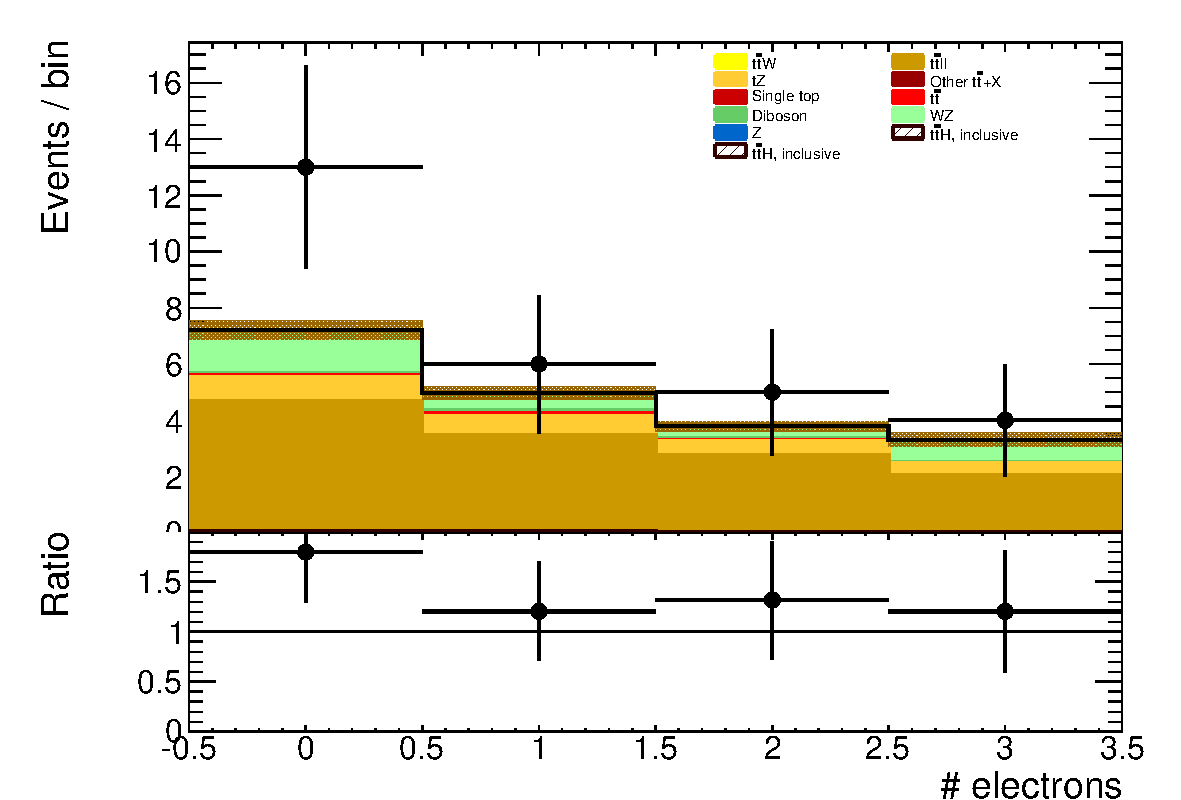
\includegraphics[width=.5\linewidth]{figs/ttZ/ttz_3l_CR_nelec}%
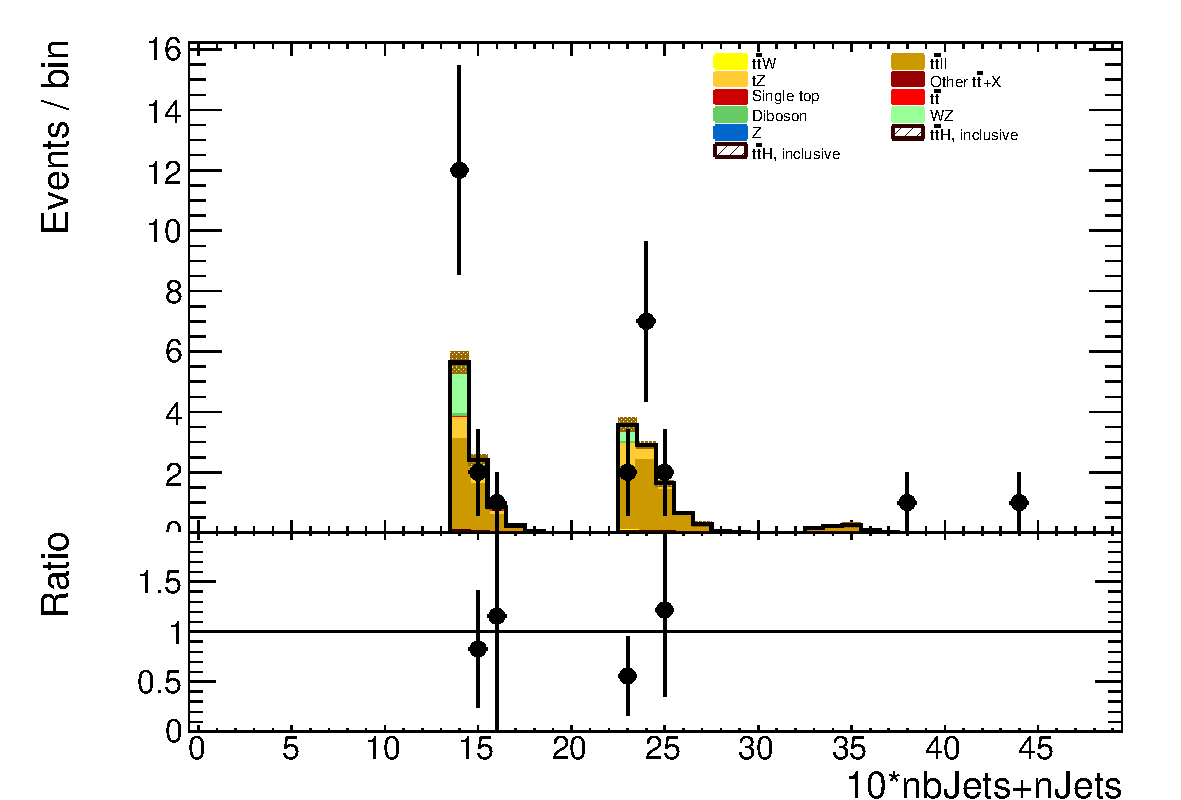
\includegraphics[width=.5\linewidth]{figs/ttZ/ttz_3l_CR_nJets_and_nbJets_lin}\\
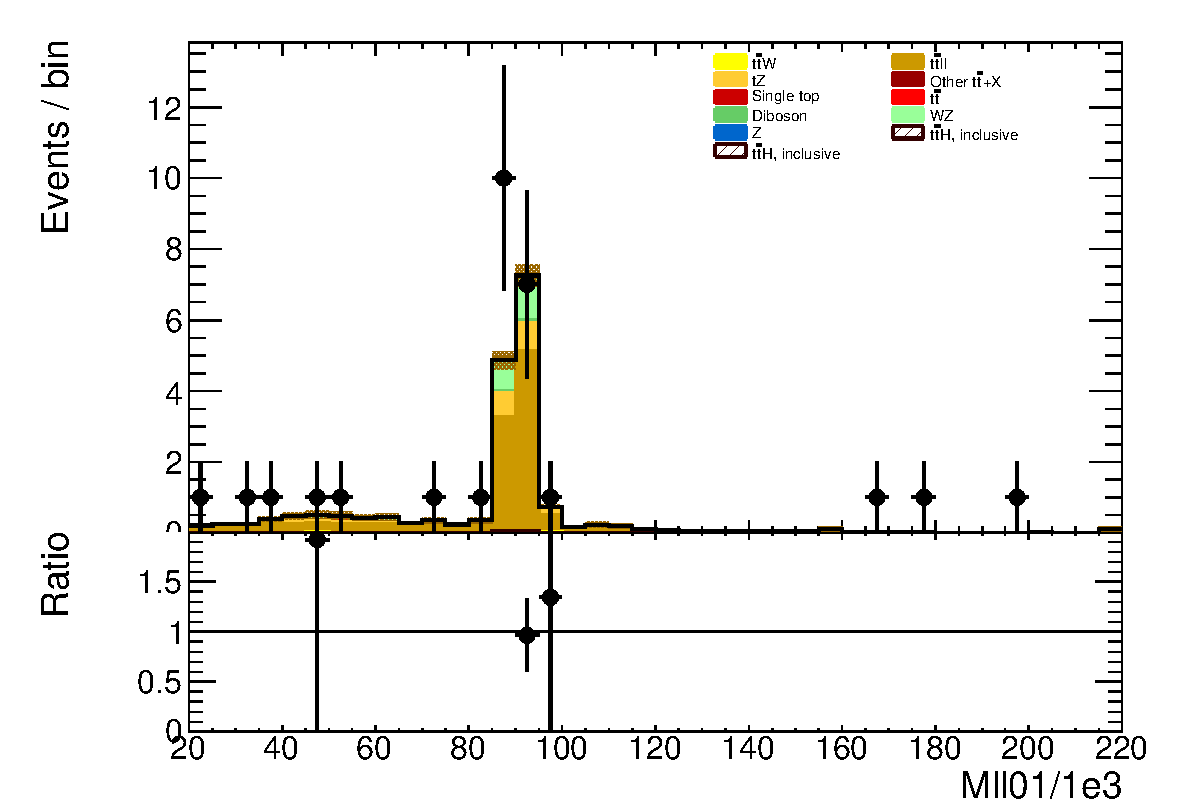
\includegraphics[width=.5\linewidth]{figs/ttZ/ttz_3l_CR_Mll01}%
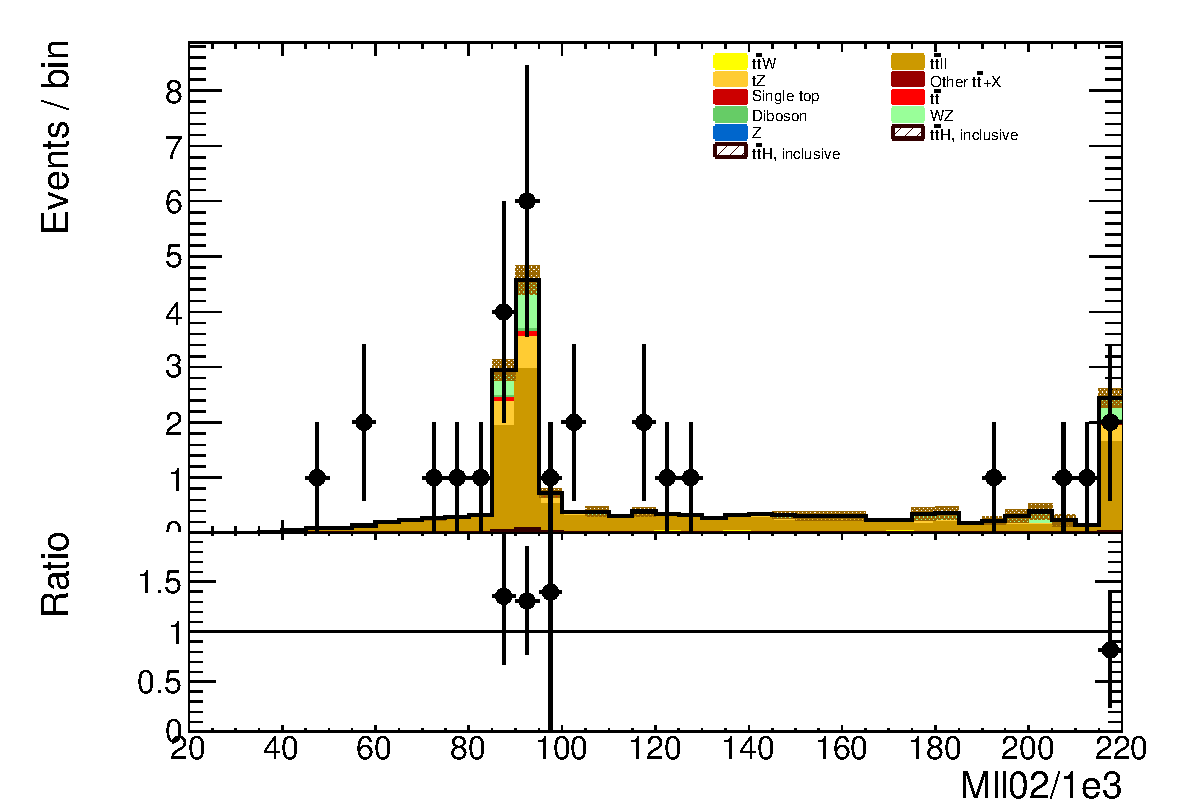
\includegraphics[width=.5\linewidth]{figs/ttZ/ttz_3l_CR_Mll02}\\
  \caption{\label{figure:background_ttZCRA}Data/MC comparison plots for \ttZ\ control region A ($\ge4$ jets, $\ge1$ $b$-tag and 3 jets, $\ge 2$ $b$-tag). In all plots, the rightmost bin contains any overflows.  Top left: number of electrons.  Top right: 10*the number of $b$-tags + the total number of jets. Middle left: the invariant mass of the (0,1) lepton pair (see the text for the definition of the lepton ordering).  Middle right: the invariant mass of the (0,2) lepton pair.}
 \end{center}
\end{figure}



\section{Di-boson Background Estimation: \WZ, \ZZ }

\label{section:wz}
$W^{\pm}Z$ and $ZZ$ di-boson production with additional and b-tagged jets constitute small contributions to 
the 3$\ell$ and 4$\ell$ channels. For the 3$\ell$ case $W^{\pm}Z$ comprises $\sim$ 10\% of the total background, while for
the 4$\ell$ case $ZZ$ contribution accounts comprises $\sim$ 10\% of the total background. 
Because of the small size of these contributions, each of the above processes can be assigned a 
non-aggressive uncertainty based on similar previous analyses with ATLAS and cross-checked with data validation 
regions and MC truth studies. 

Both $W^{\pm}Z$ and $ZZ$ production have been studied by ATLAS \cite{WZAtlas}\cite{ZZAtlas}, but neither process
has been investigated thoroughly in association with multiple jets and b-quark jets. However, single boson production with
b-quark jets has been investiaged. Both $W+b$ \cite{WbAtlas} 
and $Z+b$ \cite{ZbAtlas} production in 7 TeV data have been shown to agree with MC models to within 20-30\%. 

A single $W$ produced in association with b-tagged jets possesses a similar topology to the $W^{\pm}Z+b$ 
process at a different energy scale and has been shown to be dominated by c mis-tags and b-jets from gluon splitting 
and multiple parton interaction. The $W+b$ analysis, referenced above, uses Alpgen MC with Herwig PS modeling, only provides
results to 1 additional jet, and uses the CombNN tagger (we use MV1). Its results are therefore not directly comparable to this \tth\ analysis (where $W^{\pm}Z$ is modeled using Sherpa with massive c and b quarks). $Z+b$ production originates from slightly different diagrams than $ZZ+b$, but the sources of the b-tags are similar. The 7 TeV analysis, referenced above, provides results with Sherpa MC with an agreement of $\sim$ 30\%. However, it also used the CombNN tagger instead of MV1. Beause of the differences of the 2011 single boson analyses (type of tagger used, type of MC and tunes used), we would like to verify the general 20-30\% level of agreement in 2012 data with the simulation and tagger used in the \tth\ analysis: Sherpa MC, 2012 tunes, MV1. With the data skims available to use we are able to do this in the $Z+b$ region but not the $W+b$.  


Figure \ref{figure:background_wz_zb} shows the spectrum of the number of reconstructed and selected jets (NJet) in a 
$Z+b$ validation region, defined by 2 tight-isolated leptons within 10 \gev of the Z mass and with at 
least one b-tagged jet, using the \tth\ analysis definitions. The level of agreement in this region confirms 
at the  30\% level seen in the 7 TeV analysis, discussed above. 

\begin{figure}[!htbp]
\centering 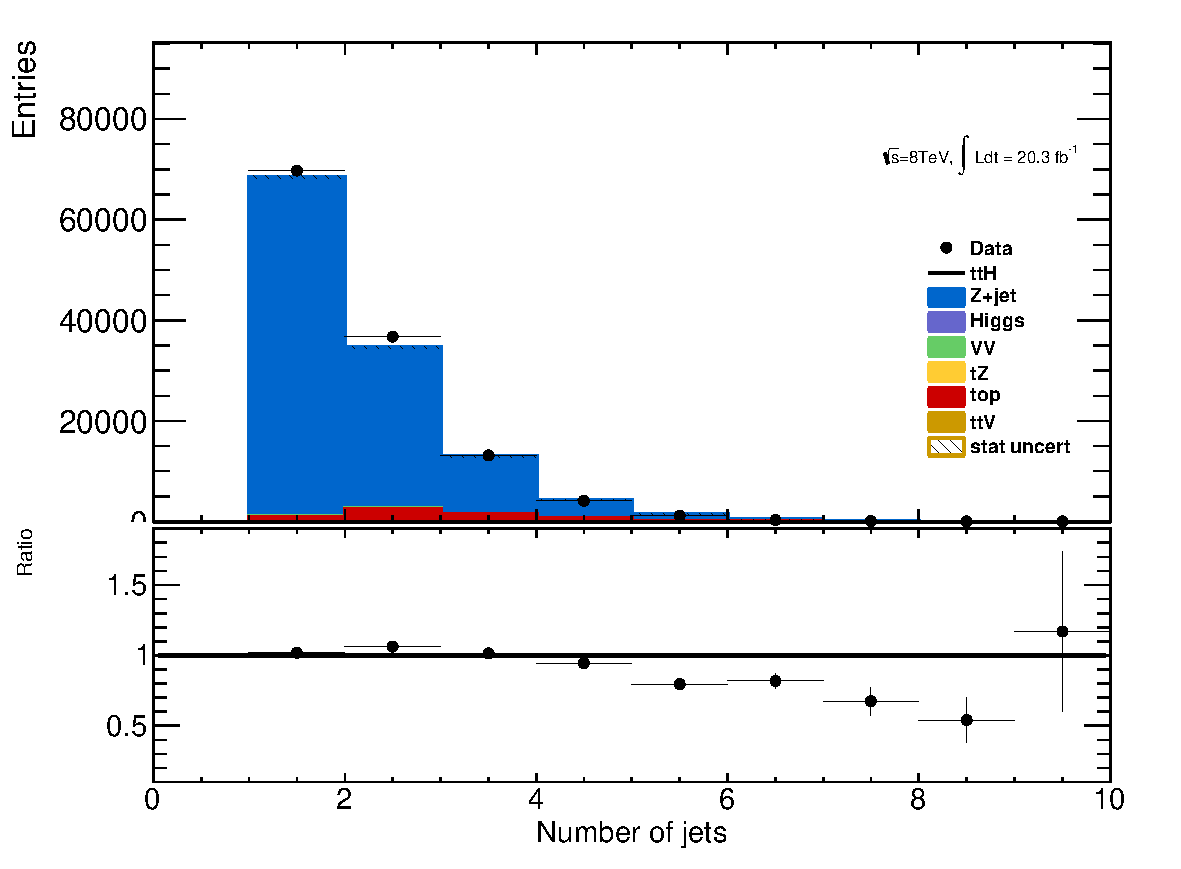
\includegraphics[width=0.5\textwidth]{figs/wz/ZbVR}
\caption{NJet spectrum for 2 tight-isolation leptons with 1 b-tagged jet (MV1\_70)} 
\label{figure:background_wz_zb}
\end{figure} 

In the following two sections, we assess the truth origin of jets in the $W^{\pm}Z+b$ and $ZZ+b$ regions and leverage data/MC agreement where we can. We see that the data allows us to constrain the \WZ\ to 50\%. We claim this 50\% as a systematic. The 20-30\% agreement in the single boson regions above bolsters our confidence in this number. 

\subsection{$W^{\pm}Z$ Normalization Uncertainty} 
The \tth\ analyses has two validation regions to test the Sherpa agreement with data for $W^{\pm}Z$: one inclusive 3 lepton region, using the three-lepton channel object and \pt\ cuts and a $W^{\pm}Z+b$ region with 1 b-tagged jet and a requirement that at least one SFOS pair have an invariant mass within 10 GeV of the Z mass. The region with fewer than 4 jets is \WZ\ dominated. Figure \ref{figure:background_wz_incl} shows kinematic variables for the inclusive region. The overall data normalization is $\sim$10\% higher than MC, but this will be well within our systematic uncertainty. The NJet shape shows good agreement across the full spectrum, giving confidence about the Sherpa high NJet SR extrapolation. Figure \ref{figure:background_wz_z_b} shows NJet spectrum for the $W^{\pm}Z+b$ validation region with agreement with in statistical uncertainties. The region has low statistics and around $\sim$ 60\% purity and statistical analysis of the region suggests that a 50\% normalization error on the \WZ\ component is enough to cover any possible mismodelings, especially in higher NJet bins, which are closer to the signal regions.  

\begin{figure}[!htbp]
  \begin{minipage}[h]{0.5\textwidth}
    \centering 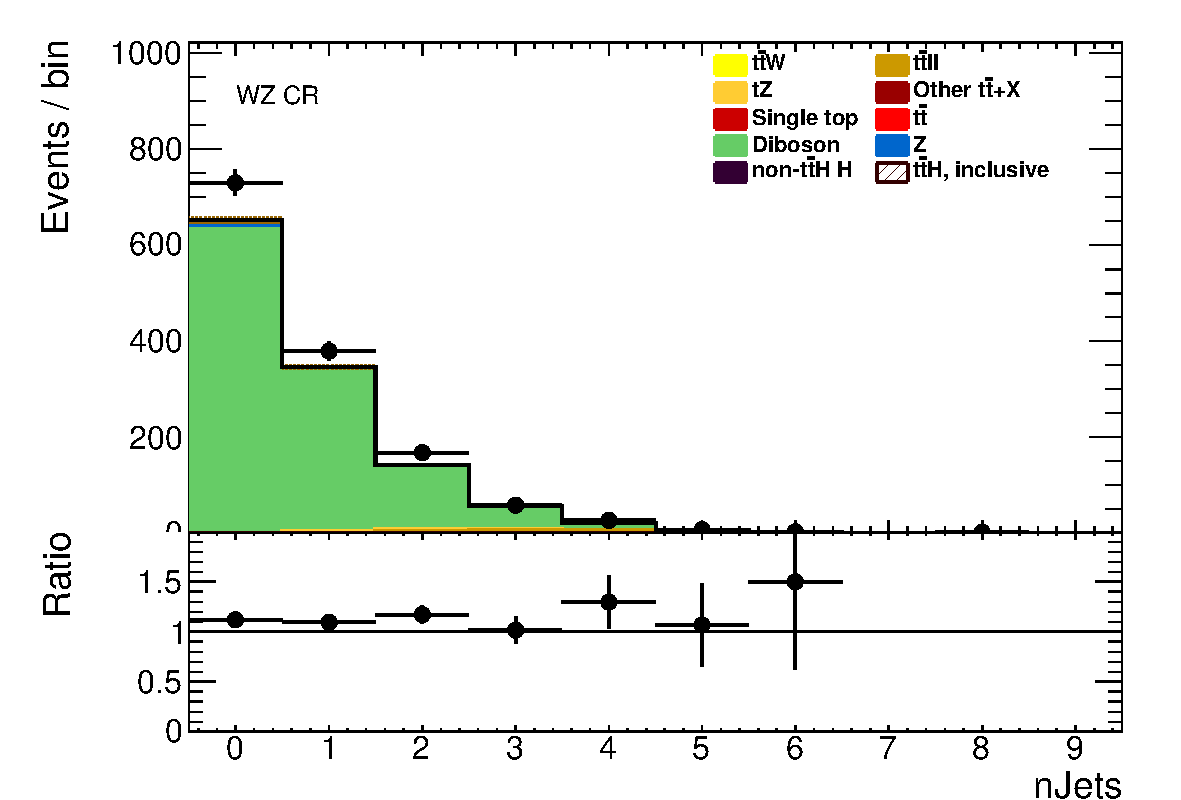
\includegraphics[width=\textwidth]{figs/WZ/standardCR_3l_WZ_MT_nJets_OR_thesis}
  \end{minipage}\hfill
  \begin{minipage}[h]{0.5\textwidth}
    \centering 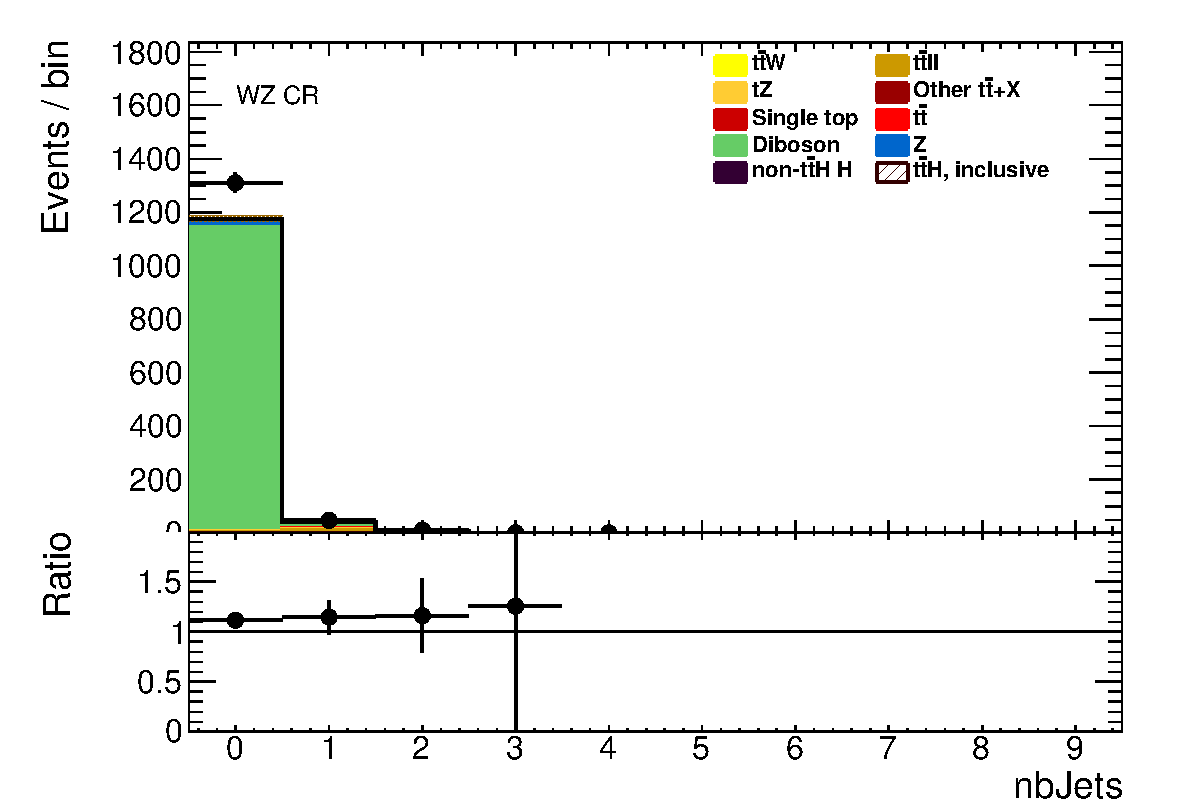
\includegraphics[width=\textwidth]{figs/WZ/standardCR_3l_WZ_MT_nJets_OR_MV1_70_thesis}
  \end{minipage}\hfill
  \begin{minipage}[h]{0.5\textwidth}
    \centering 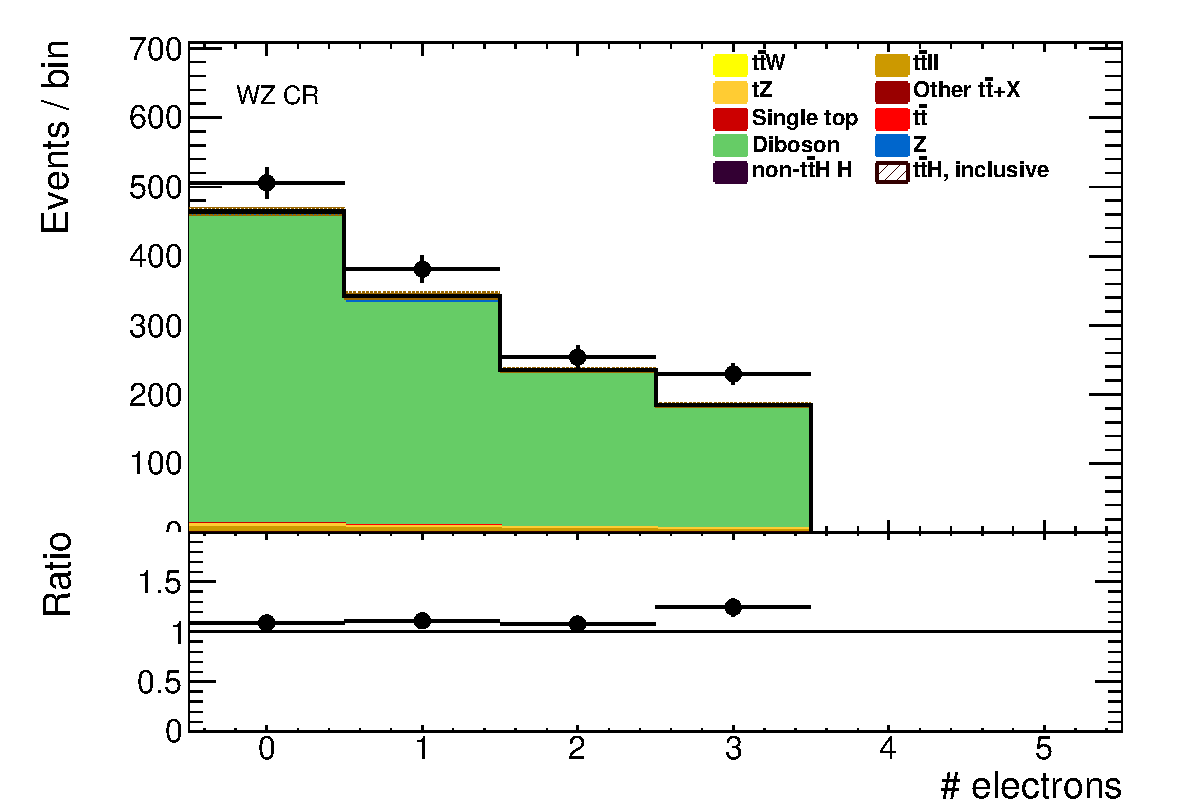
\includegraphics[width=\textwidth]{figs/WZ/standardCR_3l_WZ_MT_nelec_thesis}
  \end{minipage}\hfill
  \begin{minipage}[h]{0.5\textwidth}
    \centering 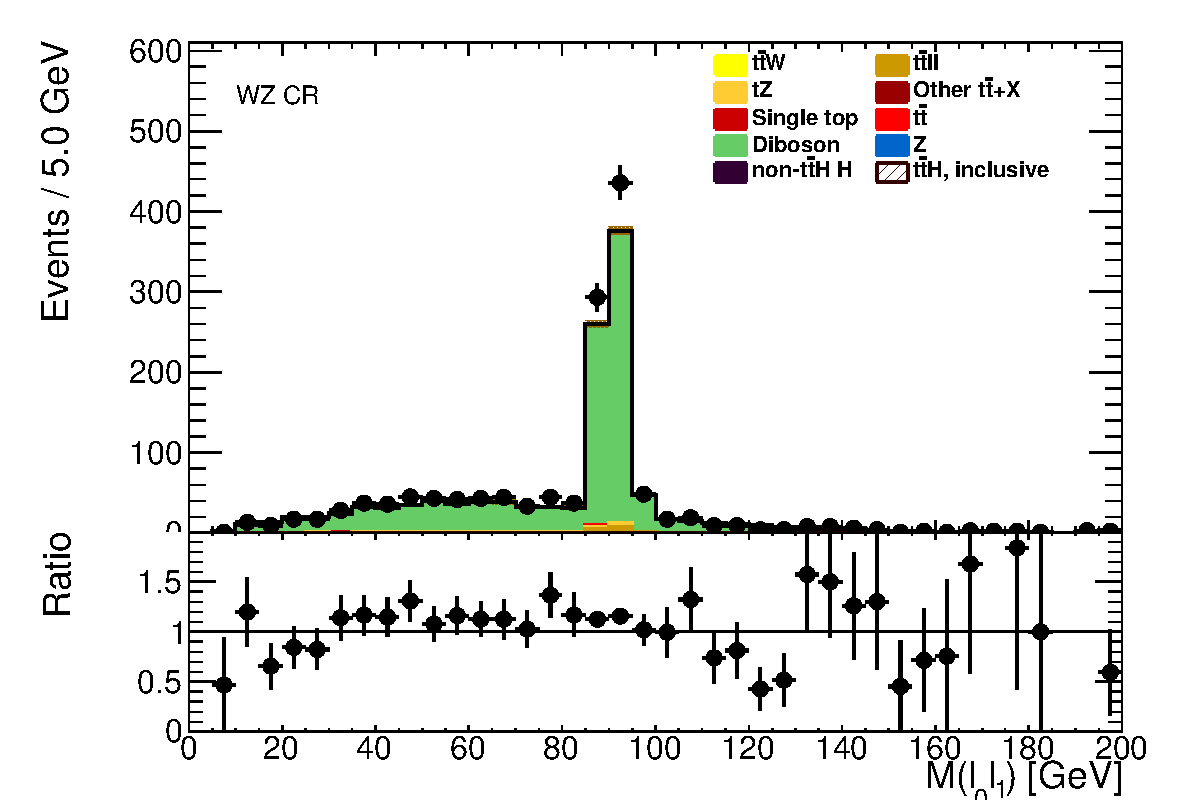
\includegraphics[width=\textwidth]{figs/WZ/standardCR_3l_WZ_MT_Mll01_thesis}
  \end{minipage}\hfill

\caption{3 lepton $W^{\pm}Z$ validation using the \tth\ lepton identification and momentum cuts: mass, number of jet and flavor variables} 
\label{figure:background_wz_incl}
\end{figure} 



\begin{figure}[!htbp]

  \begin{minipage}[h]{0.5\textwidth}
    \centering 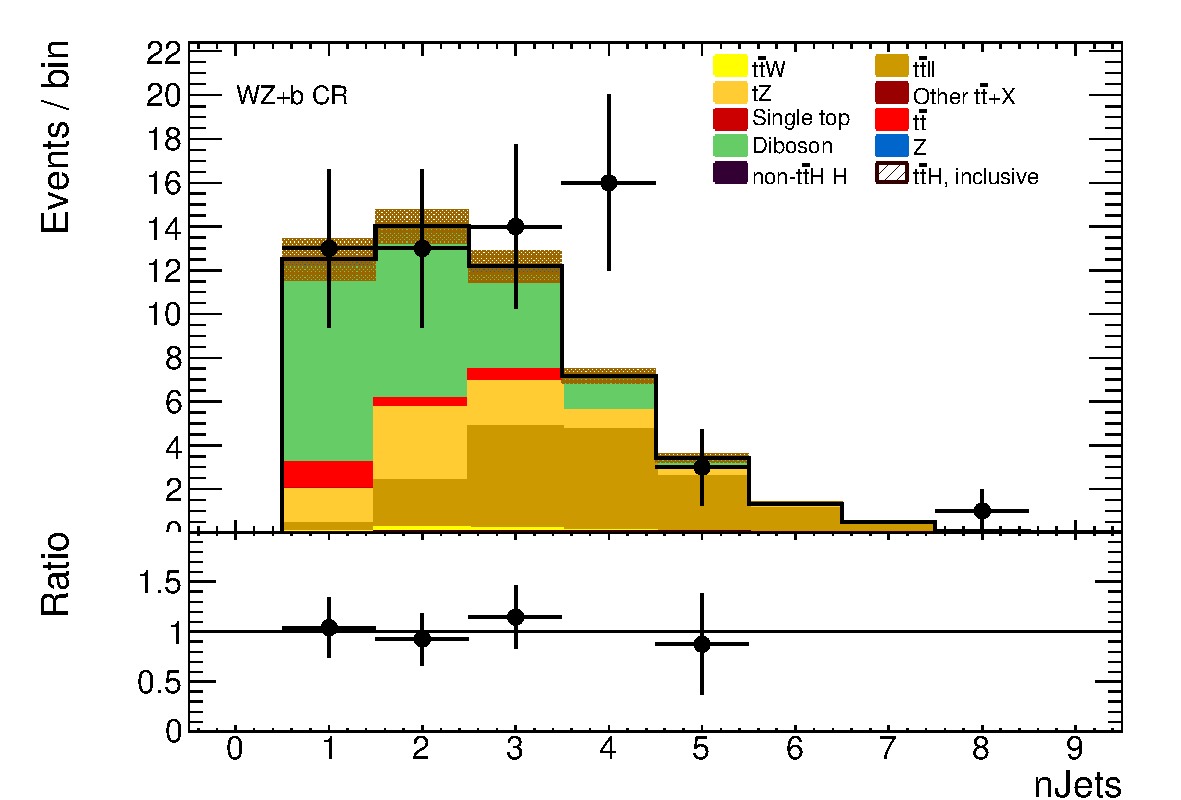
\includegraphics[width=\textwidth]{figs/WZ/standardCR_3l_WZ_MT_1b_nJets_OR_thesis}
  \end{minipage}\hfill
  \begin{minipage}[h]{0.5\textwidth}
    \centering 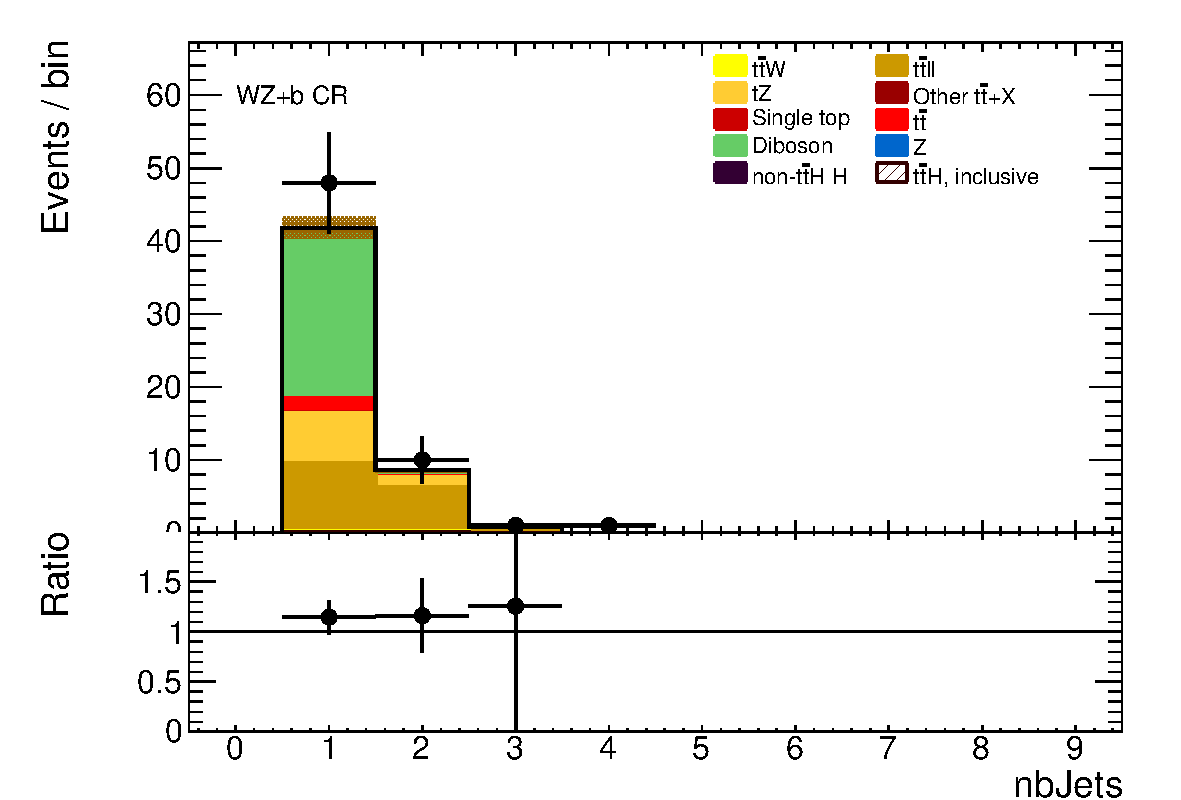
\includegraphics[width=\textwidth]{figs/WZ/standardCR_3l_WZ_MT_1b_nJets_OR_MV1_70_thesis}
  \end{minipage}\hfill
  \begin{minipage}[h]{0.5\textwidth}
    \centering 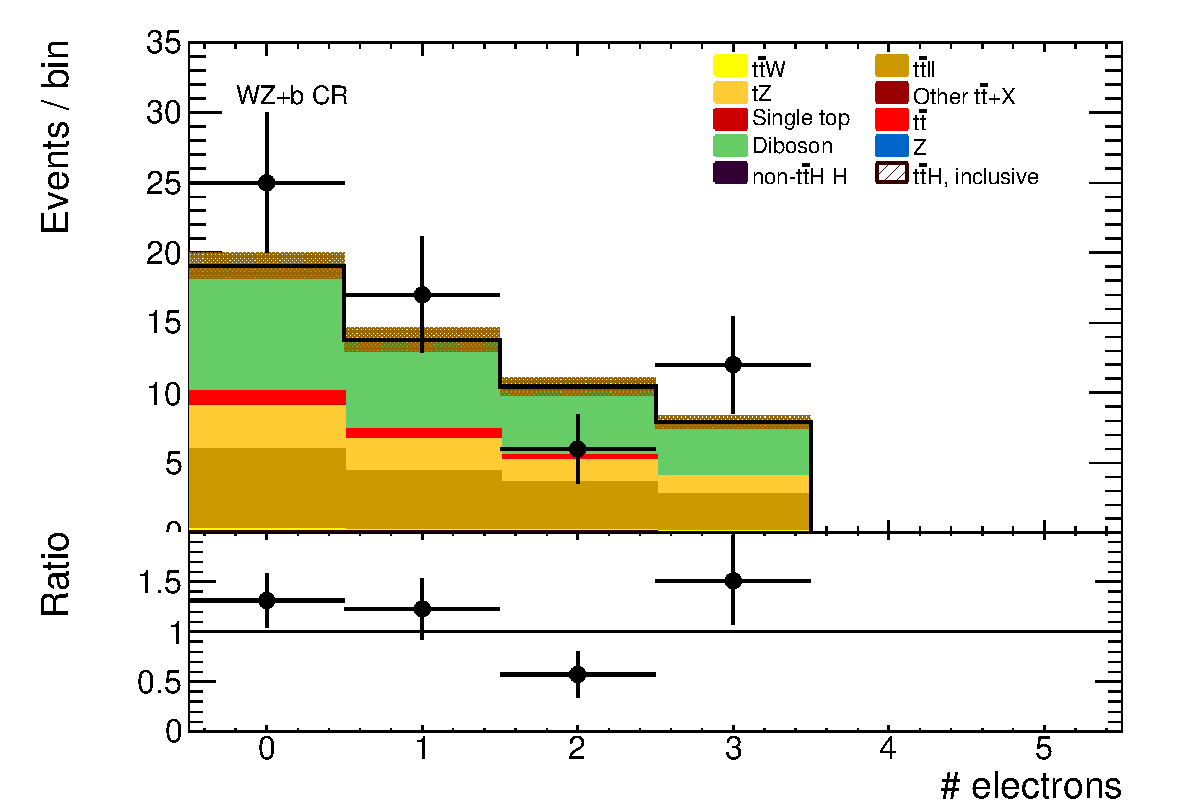
\includegraphics[width=\textwidth]{figs/WZ/standardCR_3l_WZ_MT_1b_nelec_thesis}
  \end{minipage}\hfill
  \begin{minipage}[h]{0.5\textwidth}
    \centering 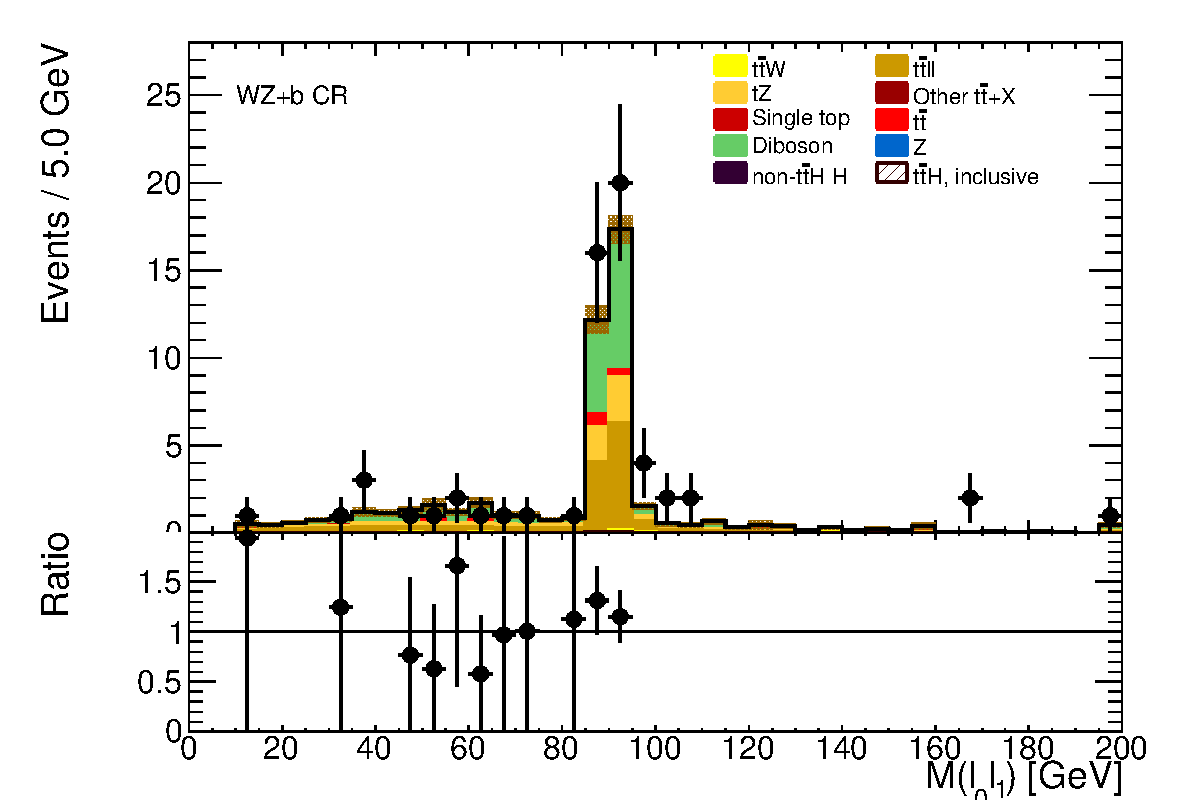
\includegraphics[width=\textwidth]{figs/WZ/standardCR_3l_WZ_MT_1b_Mll01_thesis}
  \end{minipage}\hfill
\caption{$W^{\pm}Z+b$ validation region: NJet, NElec, and Mass Variables} 
\label{figure:background_wz_z_b}
\end{figure} 

We also examine the $W^{\pm}Z$ truth origins of the b-jet in the $W^{\pm}Z+b$ validation region (VR) and the signal region using MC to assess the validity of the extrapolation from the VR to the SR and to confirm the similarity in jet origin to the single boson analyses, references above. The flavour of the closest matching truth particle ($p_T > 5$ GeV, after FSR) in $\Delta R$ determines the true-jet flavor. If there are no quarks, taus or gluons within $\Delta R$ of 0.3, the label defaults to light.  Table \ref{table:wz_truth} shows the origin fraction of b-tagged jets in the various $W^{\pm}Z+b$ VRs and the SR. If there are two b-tagged jets, the highest \pt\ is used, but this is a small fraction of the number of b-tags. As expected the c and b contributions dominate, as was the case with the 2011 single boson analyses referenced above. It is important also that the VR has similar composition to the SR.  There is a small dependence on the number of jets. 

\begin{table}[htbp]
\centering 
\begin{tabular}{|c|c|c|c|} 
  \hline
  & Bottom  & Charm & Light \\
  \hline
  $W^{\pm}Z+b$ VR 1 Jet& 0.25 $\pm$ 0.03 & 0.54  $\pm$ 0.04 & 0.20 $\pm$ 0.03 \\ 
  $W^{\pm}Z+b$ VR 2 Jet& 0.34 $\pm$ 0.04 & 0.52  $\pm$ 0.06 & 0.13 $\pm$ 0.03 \\ 
  $W^{\pm}Z+b$ VR 3 Jet& 0.40 $\pm$ 0.07 & 0.41  $\pm$ 0.07 & 0.18 $\pm$ 0.04 \\
  3$l$ SR              & 0.43 $\pm$ 0.14 & 0.38  $\pm$ 0.17 & 0.18 $\pm$ 0.11 \\
  \hline 
\end{tabular}
\caption{Truth origin of highest energy b-tagged jet in the $W^{\pm}Z+b$ VR and 3$l$ SR} 
\label{table:wz_truth}
\end{table} 

\subsection{$ZZ$ Normalization Uncertainty}

In order to investigate the MC agreement with data in the $ZZ$ case, two validation regions similar to the $W^{\pm}Z$ case are defined. First, a 4 lepton $ZZ$ region is constructed using the object selections for the 4-lepton channel and requiring exactly two pairs of 
SFOS leptons with a di-lepton invariant mass within 10 GeV of the $Z$ mass. Additionally, the $ZZ+b$ process 
is investigated directly using a similar validation region which again requires exactly two Z-candidate lepton pairs as well as at least 1 b-tagged jet. Some kinematic distributions are shown in Figures \ref{figure:background_zz_incl} and \ref{figure:background_zz_z_b}, and particular attention should be paid to the NJet spectrum, which shows good data-MC agreement in the high-jet bins, with a slight discrepancy in the 1-jet bin. The agreement for the region with at least 2 jets yields confidence in the NJet MC modeling in this region which lies close to the 4-lepton signal region. 

\begin{figure}[htbp]
  \begin{minipage}[h]{0.5\textwidth}
    \centering \includegraphics[width=\textwidth]{figs/WZ/plotCand_4lep_ZZ_CR_Njet}
  \end{minipage}\hfill
  \begin{minipage}[h]{0.5\textwidth}
    \centering 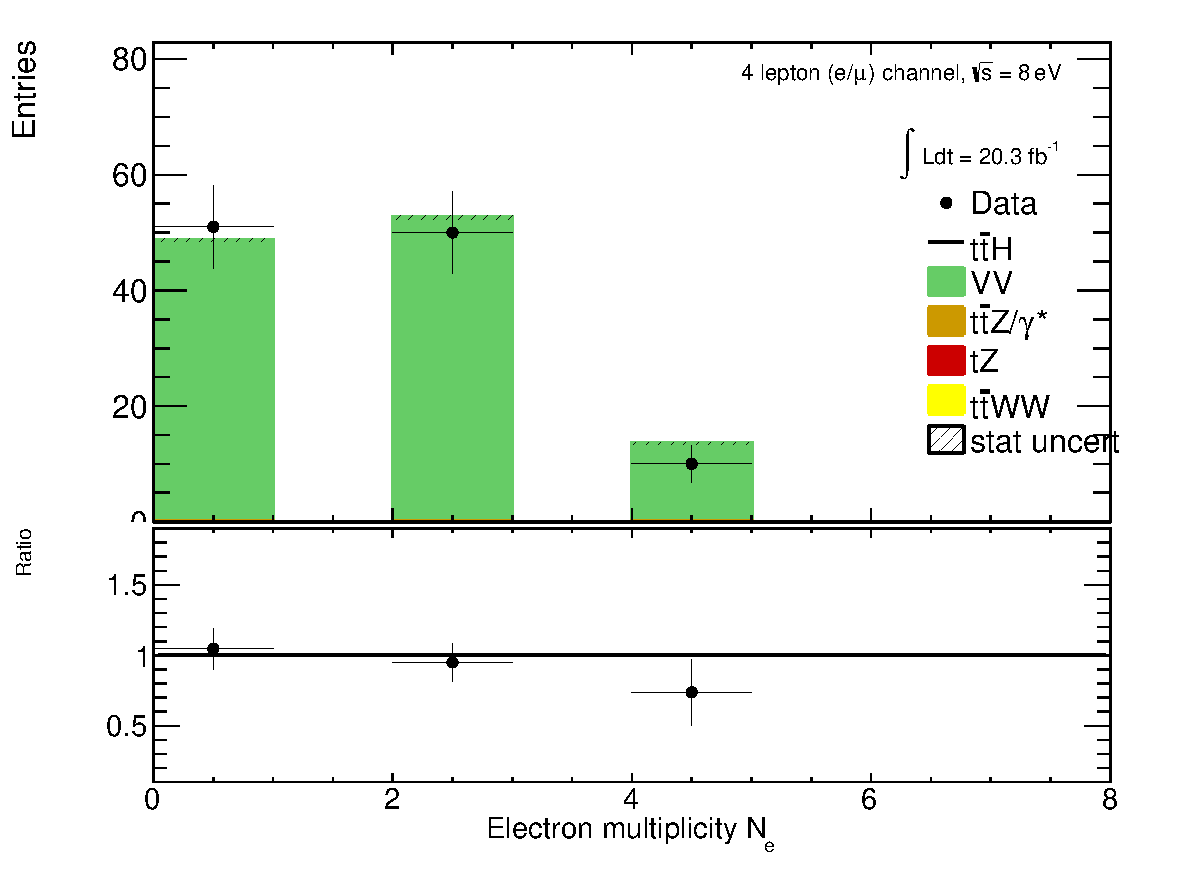
\includegraphics[width=\textwidth]{figs/WZ/plotCand_4lep_ZZ_CR_NElec}
  \end{minipage}\hfill
  \begin{minipage}[h]{0.5\textwidth}
    \centering 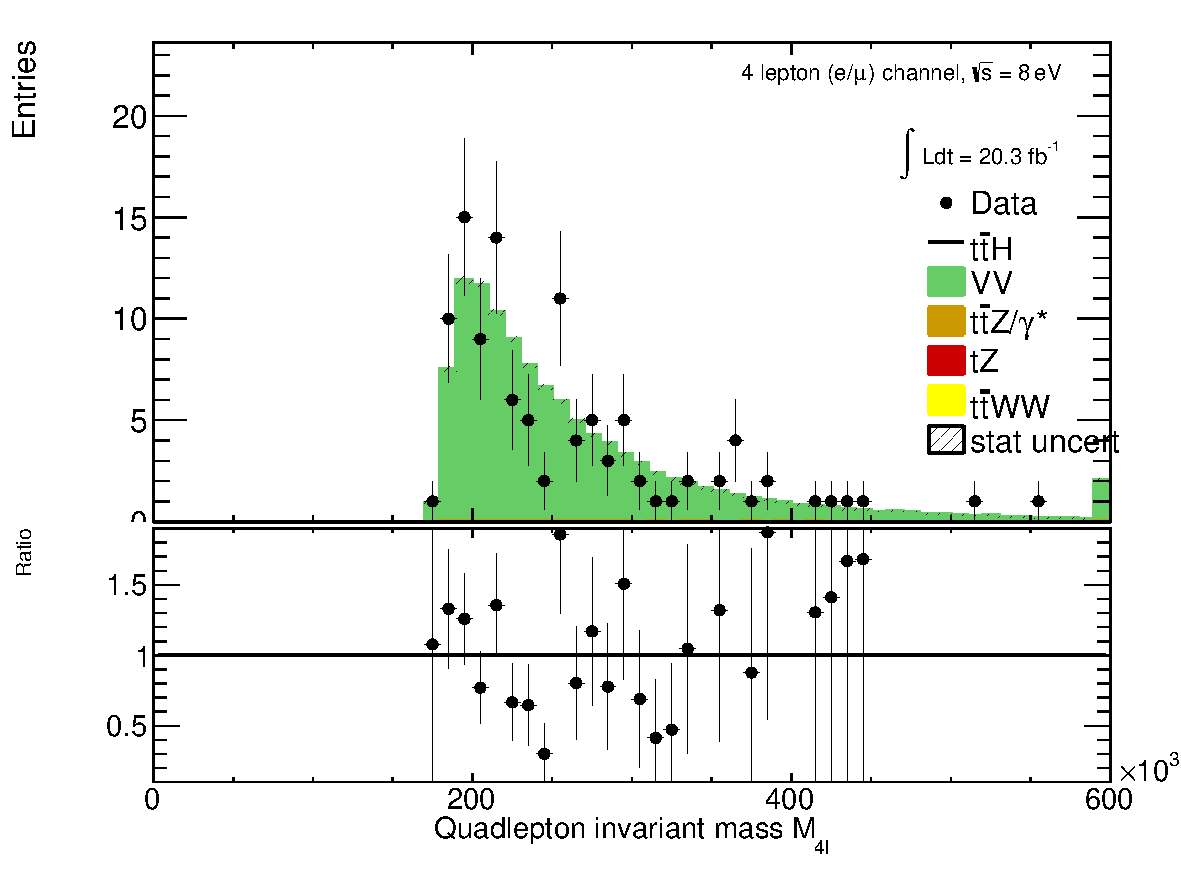
\includegraphics[width=\textwidth]{figs/WZ/plotCand_4lep_ZZ_CR_Mllll}
  \end{minipage}\hfill
  \begin{minipage}[h]{0.5\textwidth}
    \centering 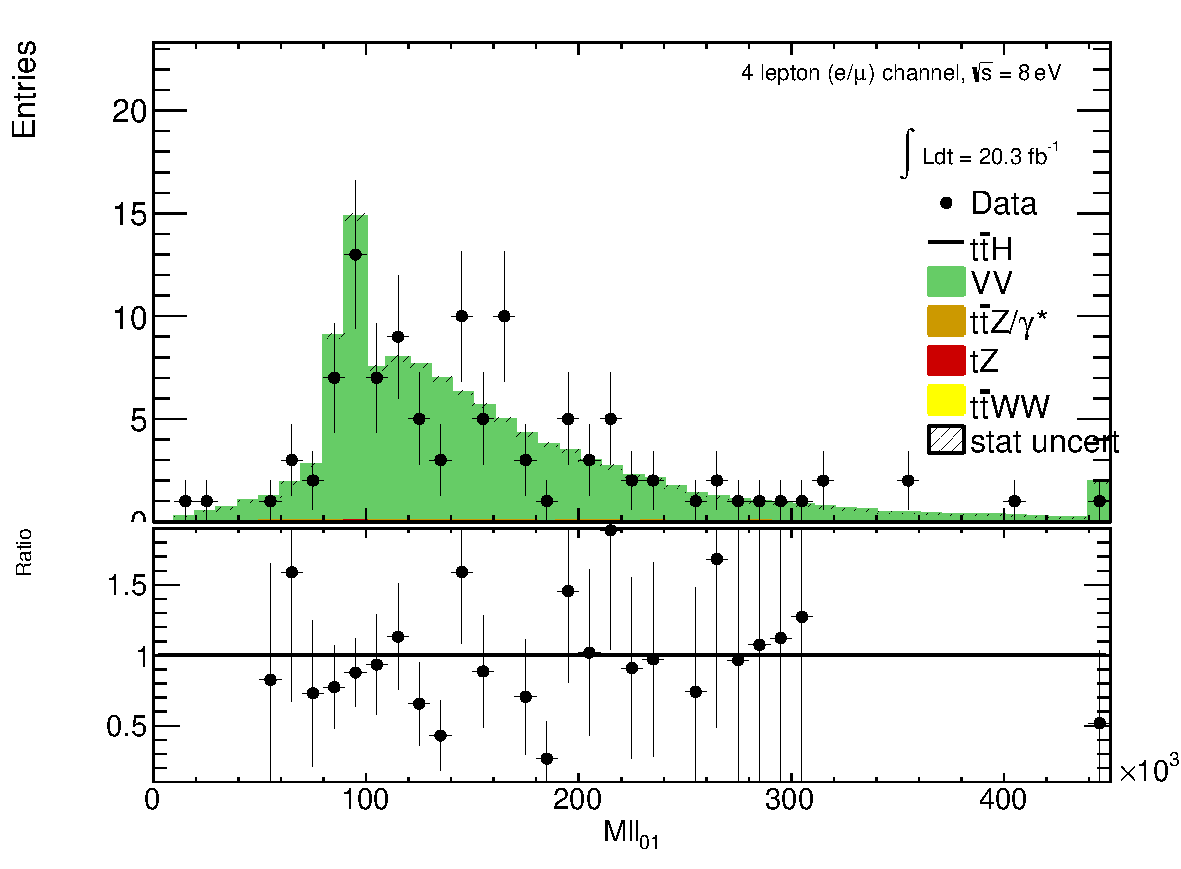
\includegraphics[width=\textwidth]{figs/WZ/plotCand_4lep_ZZ_CR_Mll01}
  \end{minipage}\hfill

  \caption{Jet-inclusive 4-lepton $ZZ$ validation region using the \tth\ lepton identification and momentum cuts }
  \label{figure:background_zz_incl}
\end{figure}


\begin{figure}[htbp]
  \begin{minipage}[h]{0.5\textwidth}
    \centering 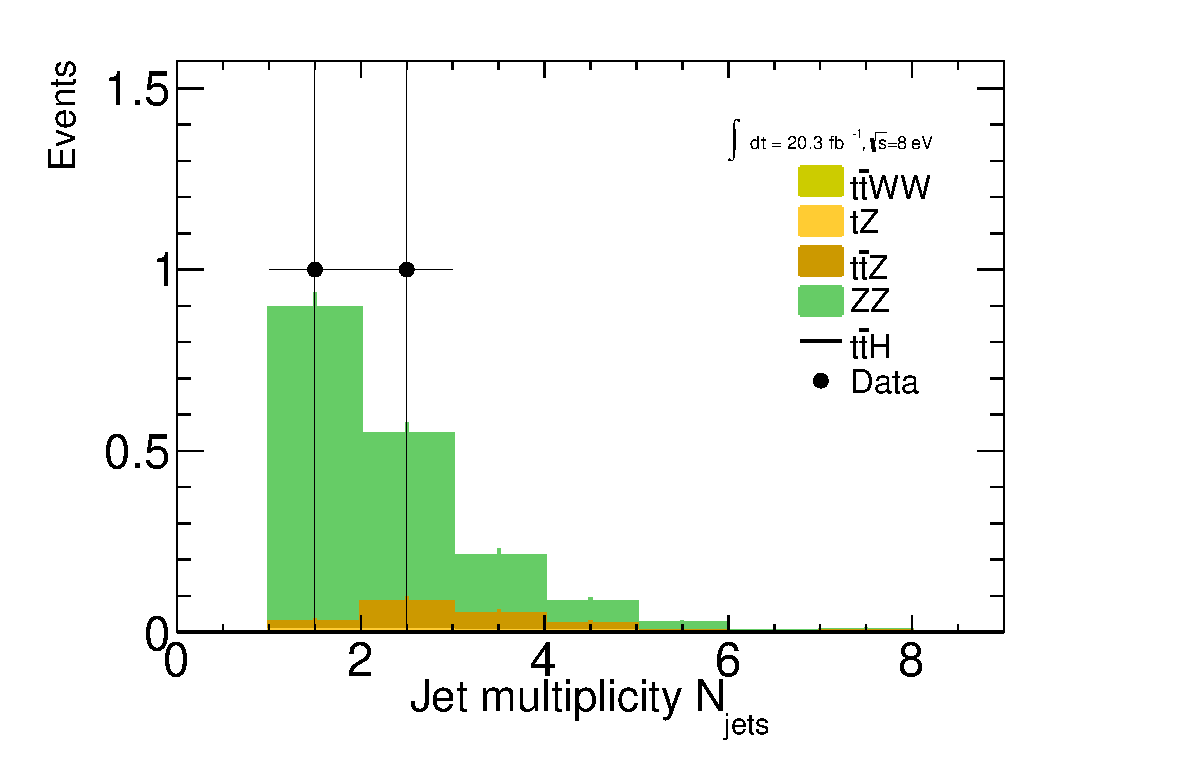
\includegraphics[width=\textwidth]{figs/WZ/zz_b_NJet}
  \end{minipage}\hfill
  \begin{minipage}[h]{0.5\textwidth}
    \centering 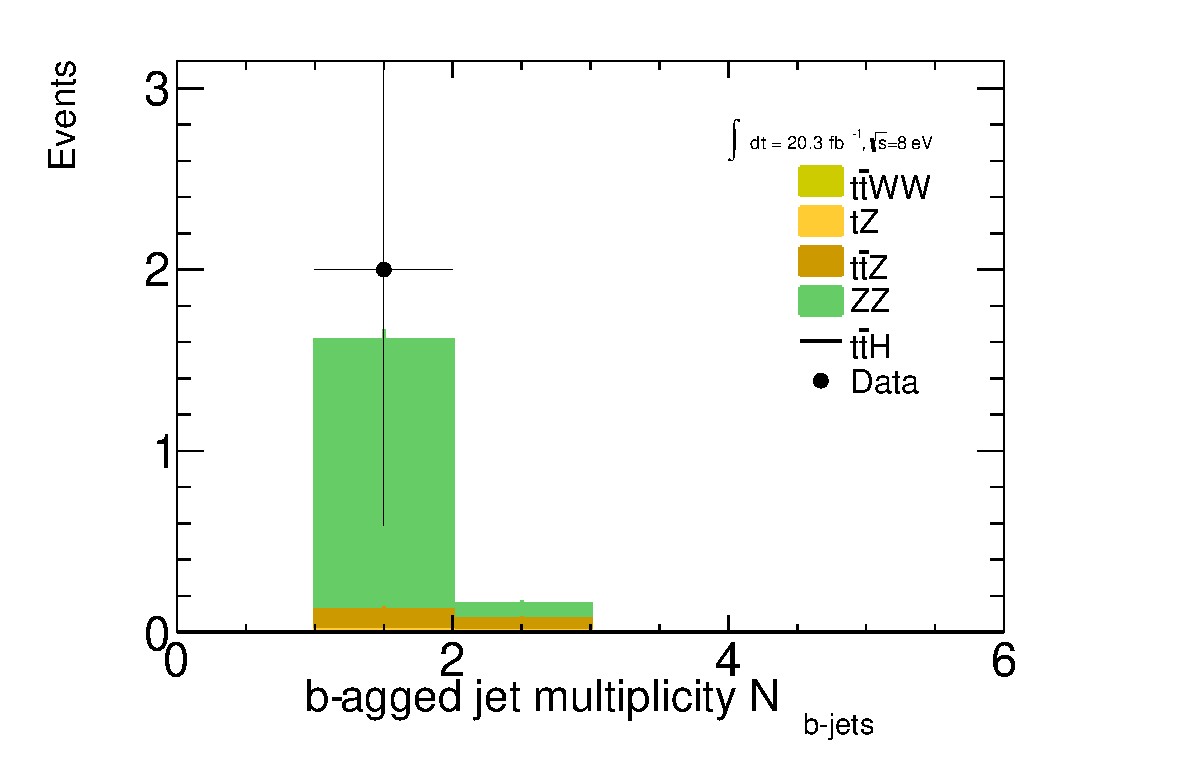
\includegraphics[width=\textwidth]{figs/WZ/zz_b_NJetBTag}
  \end{minipage}\hfill
        \caption{$ZZ+b$ validation region using the \tth\ lepton identification and momentum cuts }
        \label{figure:background_zz_z_b}
\end{figure}
 
Based on the study of the $ZZ$ and $ZZ+b$ validation regions and the overall agreement noted with the $Z+b$ analysis, we expect a similar error to \WZ\ to be appropriate in the $ZZ$ case.  A truth origin study is undertaken in MC to demonstrate a similar b-jet origin to the $W^{\pm}Z$ case. The true origin of the leading (highest energy) b-tagged jet is shown in Table \ref{table:zz_truth} for the 4-lepton signal region as well as the $ZZ+b$ validation region described above divided into jet bins. As it was in the $W^{\pm}Z$ case above, the true origin of the b-jet in $ZZ+b$ is dominated by c and b. Taking this study in tandem with the results from the $W^{\pm}Z$ investigation, it is appropriate to take the central value of the $ZZ+b$ background contribution in the 4-lepton SR from MC and to assign an overall systematic of 50\% in order to account for the MC modeling limitations. 

\begin{table}[htbp]
\centering 
\begin{tabular}{|c|c|c|c|} 
  \hline
                 & Bottom      & Charm       & Light \\
  \hline
  $ZZ+b$ VR 1 Jet& 0.56 $\pm$ 0.03 & 0.24 $\pm$ 0.01 & 0.20 $\pm$ 0.01 \\ 
  $ZZ+b$ VR 2 Jet& 0.52 $\pm$ 0.05 & 0.25 $\pm$ 0.02 & 0.23 $\pm$ 0.02 \\ 
  $ZZ+b$ VR 3 Jet& 0.53 $\pm$ 0.11 & 0.25 $\pm$ 0.08 & 0.22 $\pm$ 0.07 \\
  4$l$ SR        & 0.34 $\pm$ 0.15 & 0.42 $\pm$ 0.16 & 0.24 $\pm$ 0.10 \\
  \hline 
\end{tabular}
\caption{Truth origin of highest energy b-tagged jet in the $ZZ+b$ VR and 4$l$ SR} 
\label{table:zz_truth}
\end{table} 


\section{Charge-Misidentification Background }
\label{section:qmis} 
Charge-misidentification contributes to the background for 2$\ell$ SS case and only for flavor channels, which include electrons. The same-sign requirement is essential in removing large SM opposite sign-backgrounds, but because of their size even small charge misidentification rates result in contamination in same-sign regions. For the 2$\ell$ SS signal regions, charge-misidentification background arise primarily from \ttbar\ di-lepton events with a smaller contribution from leptonic $Z$ decays. 

In general, charge-misidentification can arise in two ways. The first occurs for ultra-high energy electrons and muons, which leave tracks in the detector that are too straight for the fit to determine the direction of curvature with high confidence. This type of charge misidentification is not a concern to the \tth\ multi-lepton analysis, as most of the leptons have transverse momentum $<$ 150 GeV. The second source of charge misidentification is from 'tridents', which only occurs for electrons, because their low mass allows for high rate bremsstrahlung in the detector material. In some cases, after an electron releases a photon through bremsstrahlung, the photon may convert nearby resulting in three electron tracks. The reconstruction algorithms may sometimes match the wrong track to the calorimeter energy deposit, resulting in a possible charge misidentification. As discussed in the selection, tight track-cluster geometric and energy matching requirements are applied on the electron candidates to reduce the overall rate and the electron acceptance is narrowed to ($|\eta| < 1.37$), since most of the material is concentrated more forward in the detector. 

We estimate the contribution of charge-misidentification events in our 2$\ell$ SS signal regions and relevant control regions by applying a weight per electron in the OS region with otherwise identical cuts. The weight is related to the charge-misidentification rates. We measure these rates using a likelihood method in the OS and SS $Z\rightarrow ee$ control region in data. The rate measured from these control regions is binned in electron \pt\ and $\eta$, to account for dependencies in these variables. The method, validations and associated errors are discussed in detail in the following sub-sections.


\subsection{Likelihood Method}

The number of reconstructed same-sign ($N_{ss}$) $Z\rightarrow ee$ events is related to total number of produced $Z\rightarrow ee$ ($N$) through factors related to the charge misidentification rate, $\epsilon$: 

\begin{equation}
N^{ij}_{ss} = N^{ij}(\epsilon_i + \epsilon_j - 2\epsilon_j\epsilon_i)
\end{equation}
where $\epsilon_i$ and $\epsilon_j$ are the charge misidentification rates for each electron separately. If we drop terms quardratic in $\epsilon$, we have:
\begin{equation}
N^{ij}_{ss}=N^{ij}(\epsilon_i+\epsilon_j).
\end{equation}
Although it is impossible to know event-by-event which electron's charge was misidentified, we can use a likelihood method over the whole $Z$ sample to measure how $\epsilon$ depends on the electron \pt\ and $|\eta|$. As illustration, we first consider the case, where $\epsilon$ depends on only one variable, $|\eta|$, and then generalize to the two-dimensional case of $|\eta|$ vs \pt. 

$N^{ij}_{ss}$ is described by a Poisson distribution:
\begin{equation}
f(k,\lambda)=\frac{\lambda^k e^{-\lambda}}{k!},
\end{equation}
where $k$ is the observed number of occurrences of the event, i.e. $k=N^{ij}_{ss}$, and $\lambda$ is the expected number,  i.e. $\lambda=N^{ij}(\epsilon_i+\epsilon_j)$. Thus, the probability for an observed number of same-sign $Z$ events given the sample size and charge misidentification rates is expressed by:
\begin{equation}
P(N^{ij}_{ss}|N^{ij},\epsilon_i,\epsilon_j)=\frac{[N^{ij}(\epsilon_i+\epsilon_j)]^{N_{ss}^{ij}}e^{-N^{ij}(\epsilon_i+\epsilon_j)}}{N^{ij}_{ss}!}.
\end{equation}
The likelihood $L$ for all the events is obtained by evaluating all the $|\eta|$ combinations:
\begin{equation}
L(\epsilon|N_{ss},N)=\prod_{i,j}\frac{[N^{ij}(\epsilon_i+\epsilon_j)]^{N_{ss}^{ij}}e^{-N^{ij}(\epsilon_i+\epsilon_j)}}{N^{ij}_{ss}!}.
\end{equation}
In this process, the $-\ln L$ is used in order to simplify and make easier the minimization. Terms which do not depend on the rates $\epsilon_i$ and $\epsilon_j$ are removed in this step. This way, the final function to minimize is given by the following expression:
\begin{equation}
\label{eq:like}
-\ln L(\epsilon|N_{ss},N)\approx \sum_{i,j}\ln[N^{ij}(\epsilon_i+\epsilon_j)]N^{ij}_{ss}-N^{ij}(\epsilon_i+\epsilon_j).
\end{equation}
The likelihood can be easily extended to depend on the charge misidentification rates as a function of two parameters. The probability to find a same-sign event given the rates for each electron is ($\epsilon_{i,k}+\epsilon_{j,l}$), where the two indices represent binned $|\eta|$- and $p_{\rm T}$-dependence. Thus, the Eq.~\ref{eq:like} transforms into
\begin{equation}
-\ln L(\epsilon|N_{ss},N)\approx \sum_{i,j,k,l}\ln[N^{ij,kl}(\epsilon_{i,k}+\epsilon_{j,l})]N^{ij,kl}_{ss}-N^{ij,kl}(\epsilon_{i,k}+\epsilon_{j,l}).
\end{equation}   

We use events selected within the $Z$ peak using the \tth\ electron object cuts. The events are stored in two matrices: one for the same-sign events $N^{ij,kl}_{ss}$,  and the other one for all events $N^{ij,kl}$. Small backgrounds need to be subtracted. The background subtraction is done using a simple side-band method.  This method consists in dividing the $Z$ invariant mass in three regions, i.e. $A$, $B$ and $C$, where $B$ is the central region corresponding to the $Z$ peak. The number of events is counted in the regions on the sides of the peak, i.e. $n_A$ and $n_C$, and removed  from the total number of events in the peak region $B$, $n_B$. This way, the number of signal events $N_Z$ is given by

\begin{equation}
N_Z=n_B-\frac{n_A+n_C}{2}.
\end{equation}
  
 Once the background has been subtracted, the likelihood is minimized for the 2D matrix of  $\epsilon$ bins. Knowing $\epsilon$ as a function of $|\eta|$ and \pt\ for any single electron, it is now possible to estimate the number of same-sign events from the number of opposite sign events in any sample:

\begin{itemize}
\item $N^{ss} = \frac{\epsilon_i +\epsilon_j -2\epsilon_i \epsilon_j}{1-\epsilon_i -\epsilon_j +2\epsilon_i \epsilon_j} N^{os}$ for $ee$ channels
\item $N^{ss} = \frac{\epsilon}{1-\epsilon} N^{os}$ for the $e\mu$ channels
\end{itemize}


\subsection{Results}

The charge misidentification rate is calculated in 7 $|\eta|$ bins [0.0, 0.6, 1.1, 1.37, 1.52, 1.7, 2.3, 2.47] by 4 \pt bins\ [15, 60, 90, 130, 1000] GeV. For \pt\ bins above 130 GeV, the $Z$ dataset becomes too small and the rates are calculated using \ttbar\ MC, scaled by the data-MC ratio of the rates in the lower \pt\ bins, [90-130] GeV. Figure \ref{figure:background_cf} shows the extracted rates in all bins.

\begin{figure}[ht!]
\centering
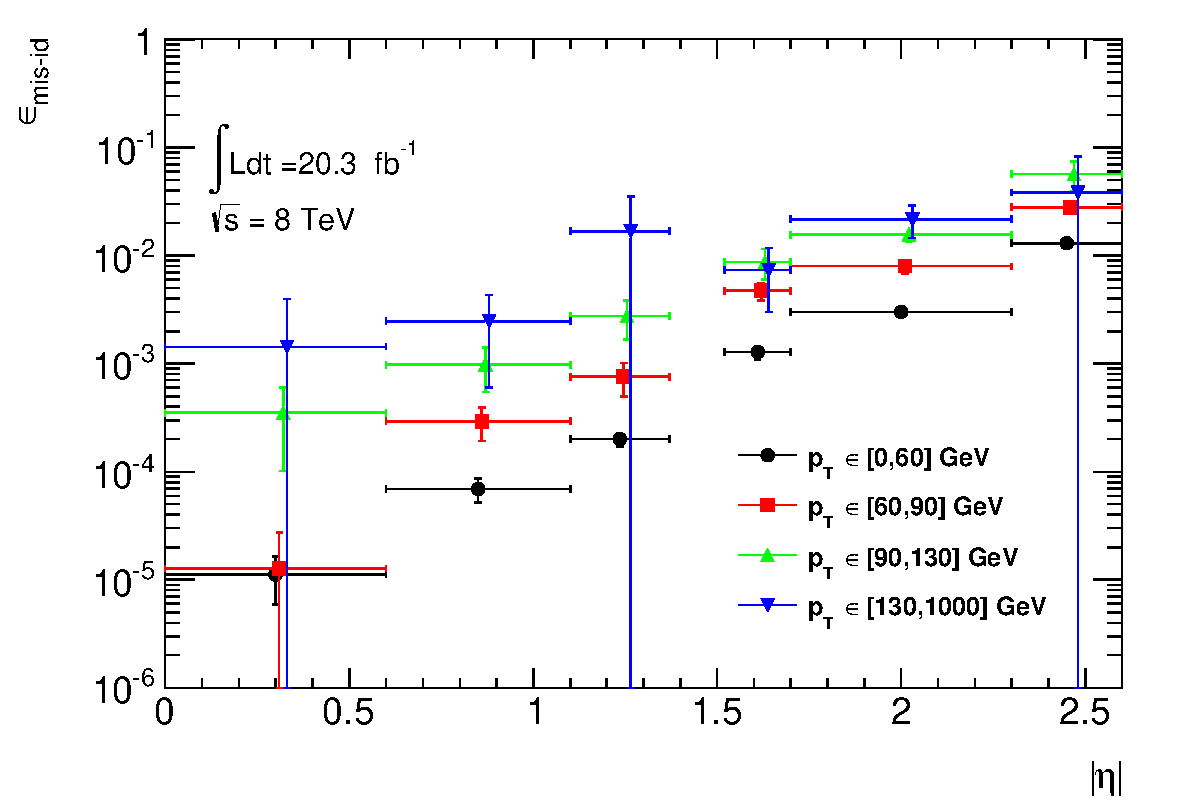
\includegraphics[width=0.7\textwidth]{figs/qmis/Rates2D}
  \caption{Electron charge misidentification rates  measured in data with the likelihood method  on $Z$ events (black points, red squares and blue triangles) as a function of $|\eta|$ and parametrized in $p_{\rm T}$. The full 2012 dataset has been used to estimate the rates below 130~GeV.   Above this value, the charge misidentification rates have been estimated by extrapolating the rates in the region where the $p_{\rm T}\in[90,130]$~GeV with a $p_{\rm T}$ dependent factor extracted from simulated $t\bar t$ events (green triangles). Statistical and systematic uncertainties  have been included in this plot. \label{figure:background_cf}}
\end{figure}


As a cross-check, we apply the full method to the $Z$ MC samples (extracting rates via a likelihood fit and applying them to opposite sign events) and compare to the MC predicted number of same-sign events. The invariant mass of the $Z$ from our charge misidentification and directly from the MC can be seen on Figure~\ref{figure:background_clMll}. In the simulated $Z$ samples, the number of same-sign $Z$ events is $5~049$ while the estimation is $5~031^{+375}_{-365}$.  The uncertainties combine both statistical systematic uncertainties, which are discussed in depth below. The validation gives compatible results within uncertainties. 
 
\begin{figure}[htb!]
\centering
\begin{minipage}[h]{0.5\textwidth}
    \centering 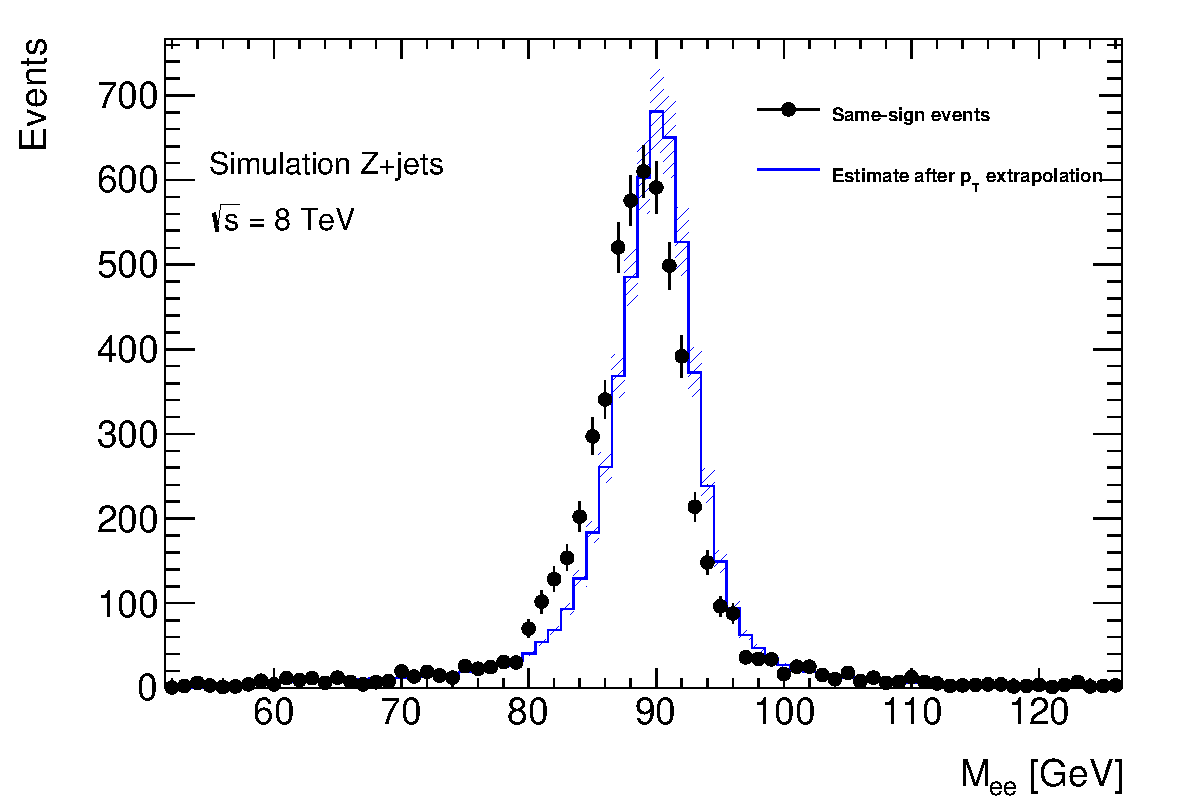
\includegraphics[width=\textwidth]{figs/qmis/ClosureMllMC}
\end{minipage}\hfill
\begin{minipage}[h]{0.5\textwidth}
    \centering 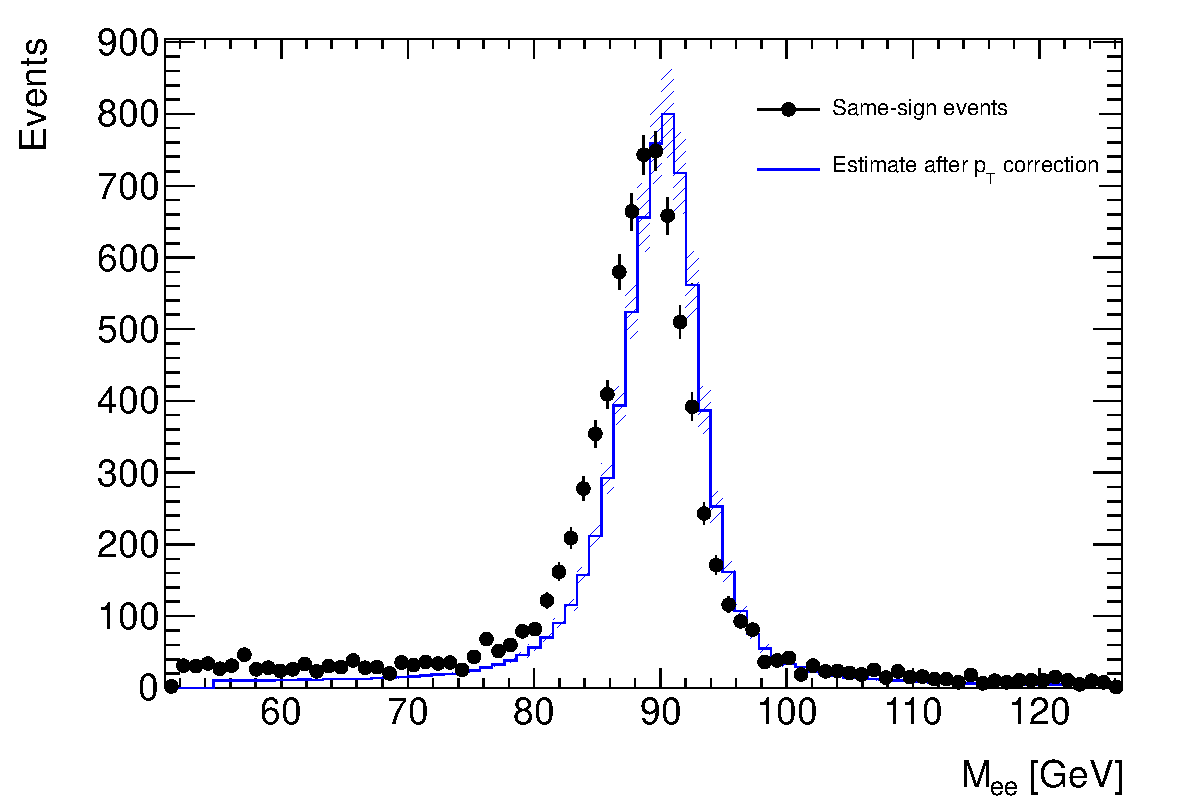
\includegraphics[width=\textwidth]{figs/qmis/ClosureMlldata}
\end{minipage}\hfill
  \caption{Closure test on simulated $Z\rightarrow e^+e^-$ events (a)   and data (b). 
      The black circles show the distribution of same-sign events while the blue histograms
      show the distribution of the re-weighted opposite-sign events together with the statistical and systematic uncertainties. The distributions are not
    expected to overlay exactly, due to the loss of energy of the trident electrons for the
    same-sign peak. \label{figure:background_clMll}}
\end{figure}


\subsection{Systematic and Statistical Uncertainties}

Statistical uncertainties dominate the combined uncertainty on the charge misidentification estimate. The statistical uncertainties come primarily from the size of the $Z$ same-sign sample in data and are especially large for central, material-poor regions where the charge misidentification rate is extremely low. Additional systematic uncertainties are included for a comparison between the positron and electron rate, the per-bin MC closure test discussed above, and for the effect of varying the invariant mass window used for the background subtraction for three different cases. Figure \ref{figure:background_qmissyst} shows the relative uncertainties for all rate bins.



 \begin{figure}[htp!] 
\centering
\setlength{\fboxrule}{0 pt}
\fbox{  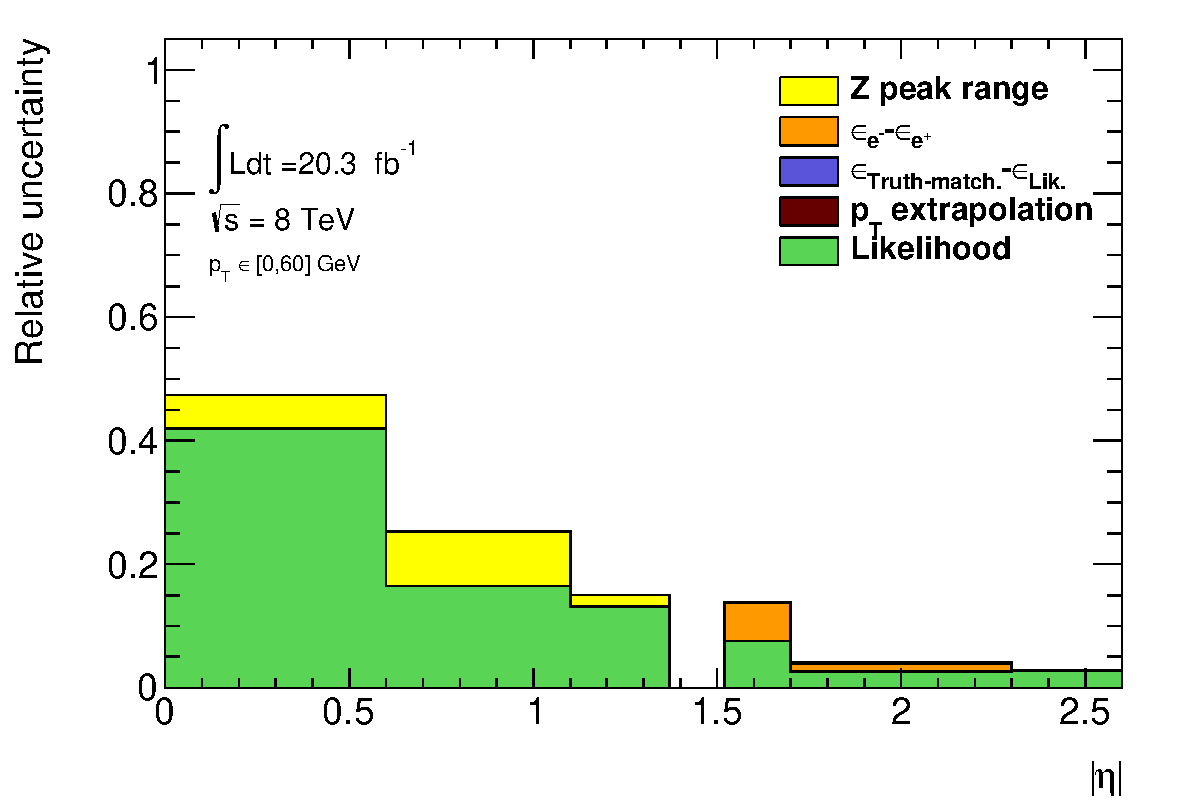
\includegraphics[width=0.48\textwidth]{figs/qmis/Syst1}}% \hspace{2cm}%
\fbox{  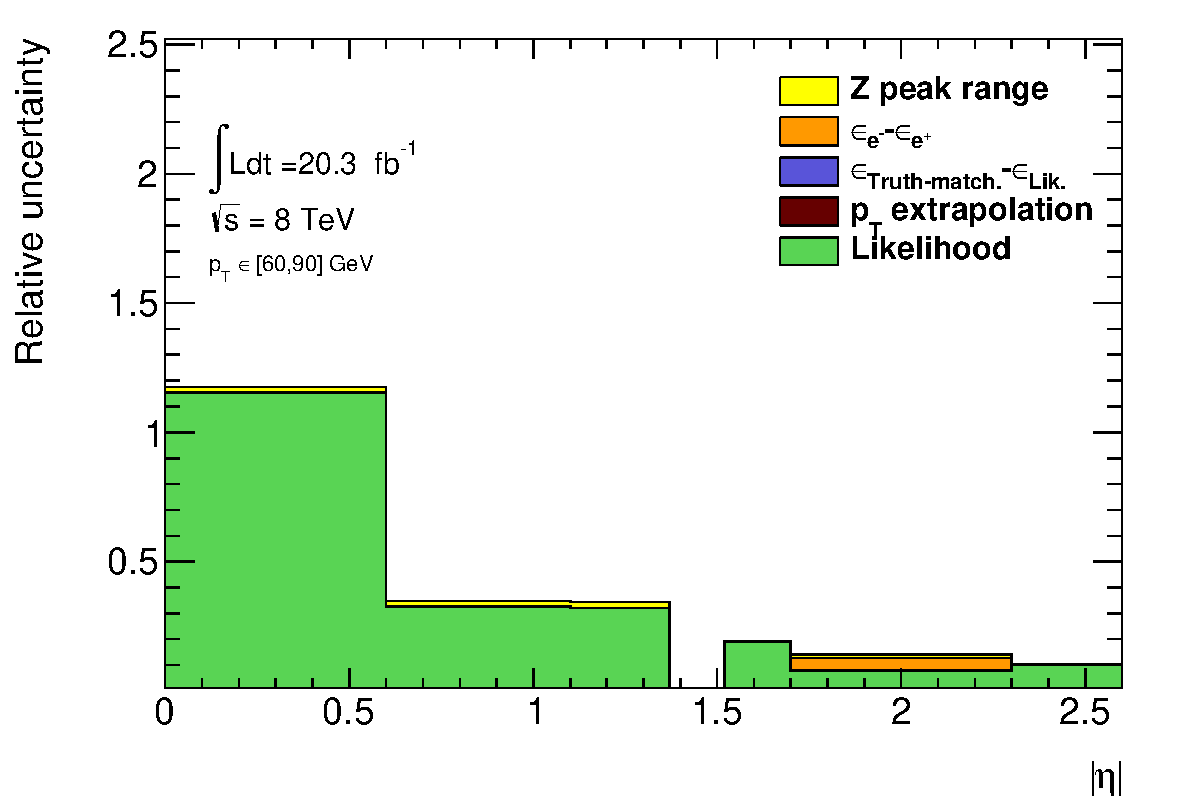
\includegraphics[width=0.48\textwidth]{figs/qmis/Syst2}}% 

\fbox{  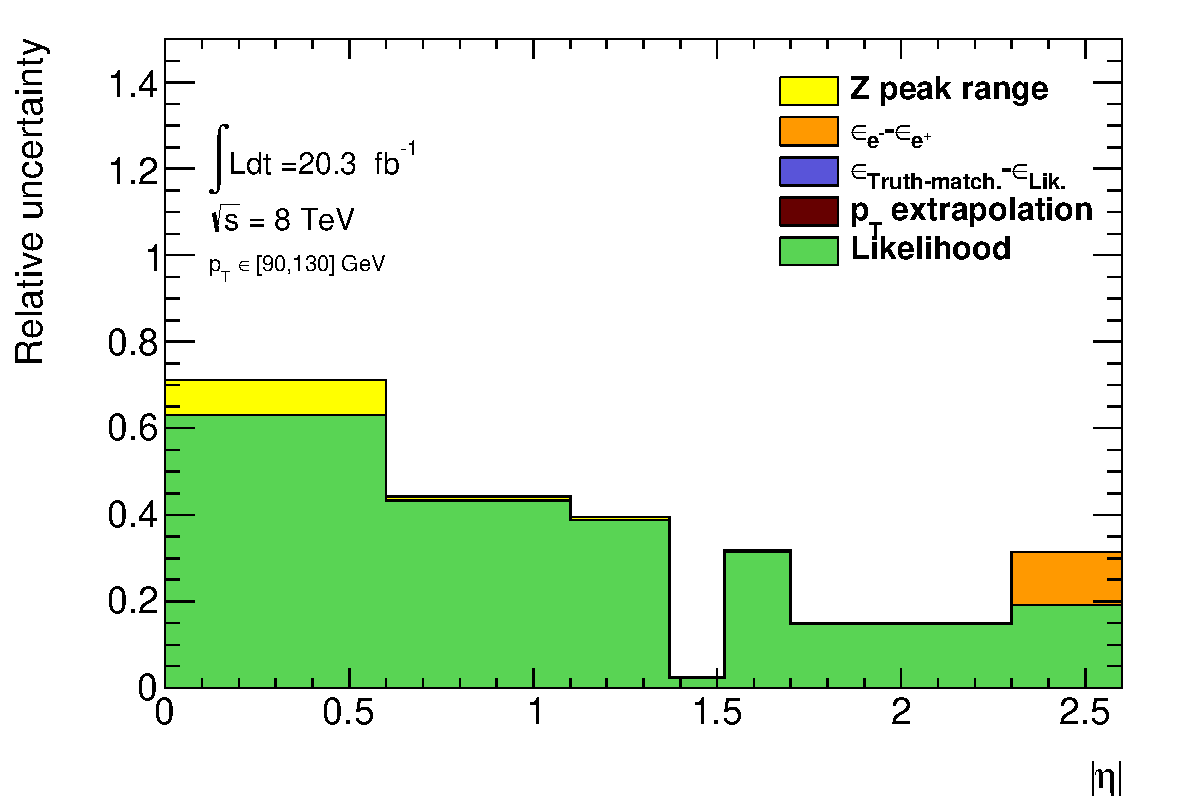
\includegraphics[width=0.48\textwidth]{figs/qmis/Syst3}}% hspace{2cm}%
\fbox{  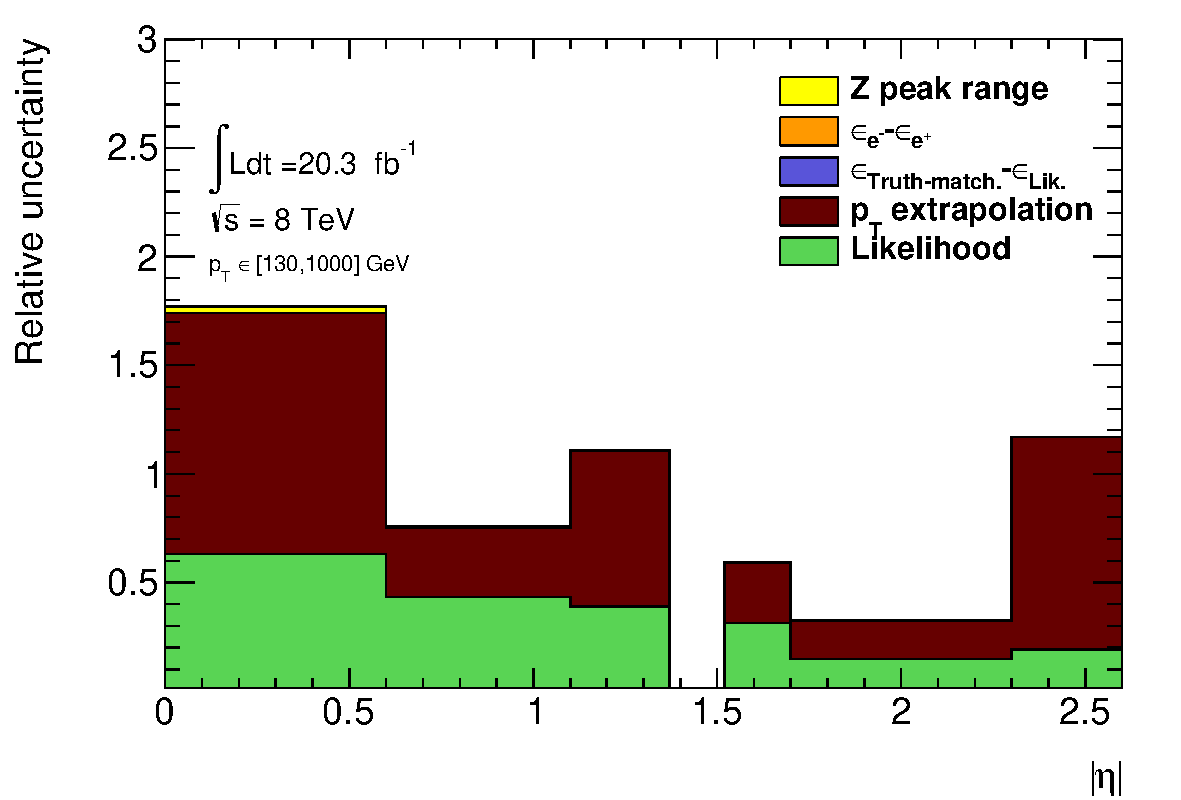
\includegraphics[width=0.48\textwidth]{figs/qmis/Syst4}}% 
\caption{Relative systematic uncertainty contributions on the
      charge misidentification rate, for different bins in $p_{\rm T}$ and 
      $|\eta|$.}\label{figure:background_qmissyst}
 \end{figure}

We apply the rates to estimate the charge misidentification background in the 2$\ell$ SS signal regions, and find  $\sim$ 25\% contamination in the \ee regions and a $\sim$ 10\% contribution to the \emu regions with a 10\% systematic error overall. The low overall error can be attributed to the fact that the statistical error is lowest where the bulk of charge misidentifications occur. The charge flip contribution measured in the signal regions from this method is detailed in Table~\ref{table:background_summary}. 


\section{Fake Lepton Backgrounds}
\label{section:fakes}
Fake Leptons, from the misidentification of jets as either electrons or muons, primarily arise from \ttbar\ and single top processes in the 2$\ell$ SS, 3$\ell$ and 4$\ell$ channels. Smaller contributions come from $Z$+jet events. Fake backgrounds are sub-dominant but important in the 2$\ell$ SS and 3$\ell$ channels. They are extremely small in the 4$\ell$ channels. Truth studies suggest that these misidentified leptons arise overwhelmingly from b-quark initiated jets. The general method for estimating fakes in all channels is to define a reversed object selection control region (usually isolation) for each lepton flavor with otherwise identical signal region selection ($N^e_{CR}$, $N^{\mu}_{CR}$). This region is fake-dominated. The total number of fake events in these regions are then scaled by transfer factors ($\theta$) to estimate the number of fake events of the appropriate flavor in the signal region. The simple formula for determining fakes is defined in Equation \ref{equation:background_total}.    


\begin{equation}
N_{fake} = \theta_e \cdot N^e_{CR} + \theta_{\mu} \cdot N^{\mu}_{CR}   
\label{equation:background_total}
\end{equation}

This approach factorizes the background model into two separate measurements. $N_{CR}$ is sensitive the overall \ttbar\ production rate, especially in the presence of additional jets from QCD ratio, as well as the object-level misidentification of a jet as a lepton. The transfer factors are sensitive to only the object level properties of the misidentified jet, and in particular only the variables which are reversed in the anti-tight identification. 

The transfer factors are obtained obtained in a different way for each channel, due to unique issues with statistics and contamination, but each method relies heavily on the data-based control regions with fewer jets. Figure \ref{figure:background_njetr} shows a truth study of the stability of the transfer factor for the 2$\ell$ SS and 3$\ell$ cases as a function of the number of jets in the event for events with one-b-tagged jet. This suggest that the regions with fewer jets are a good model of the fakes in the signal regions with more jets and is expected because of the homogeneity of origin of the fakes across all jet bins.  

The details of the methods for each channel are discussed in depth in the following sections. For all methods, the overall systematic uncertainty on the normalization of the fake estimate is in the range 30\%-50\% and arise primarily from statistics and the closure on assumptions used to obtain the transfer factor.

\begin{figure}[htbp]
\begin{minipage}[h]{0.5\textwidth}
    \centering 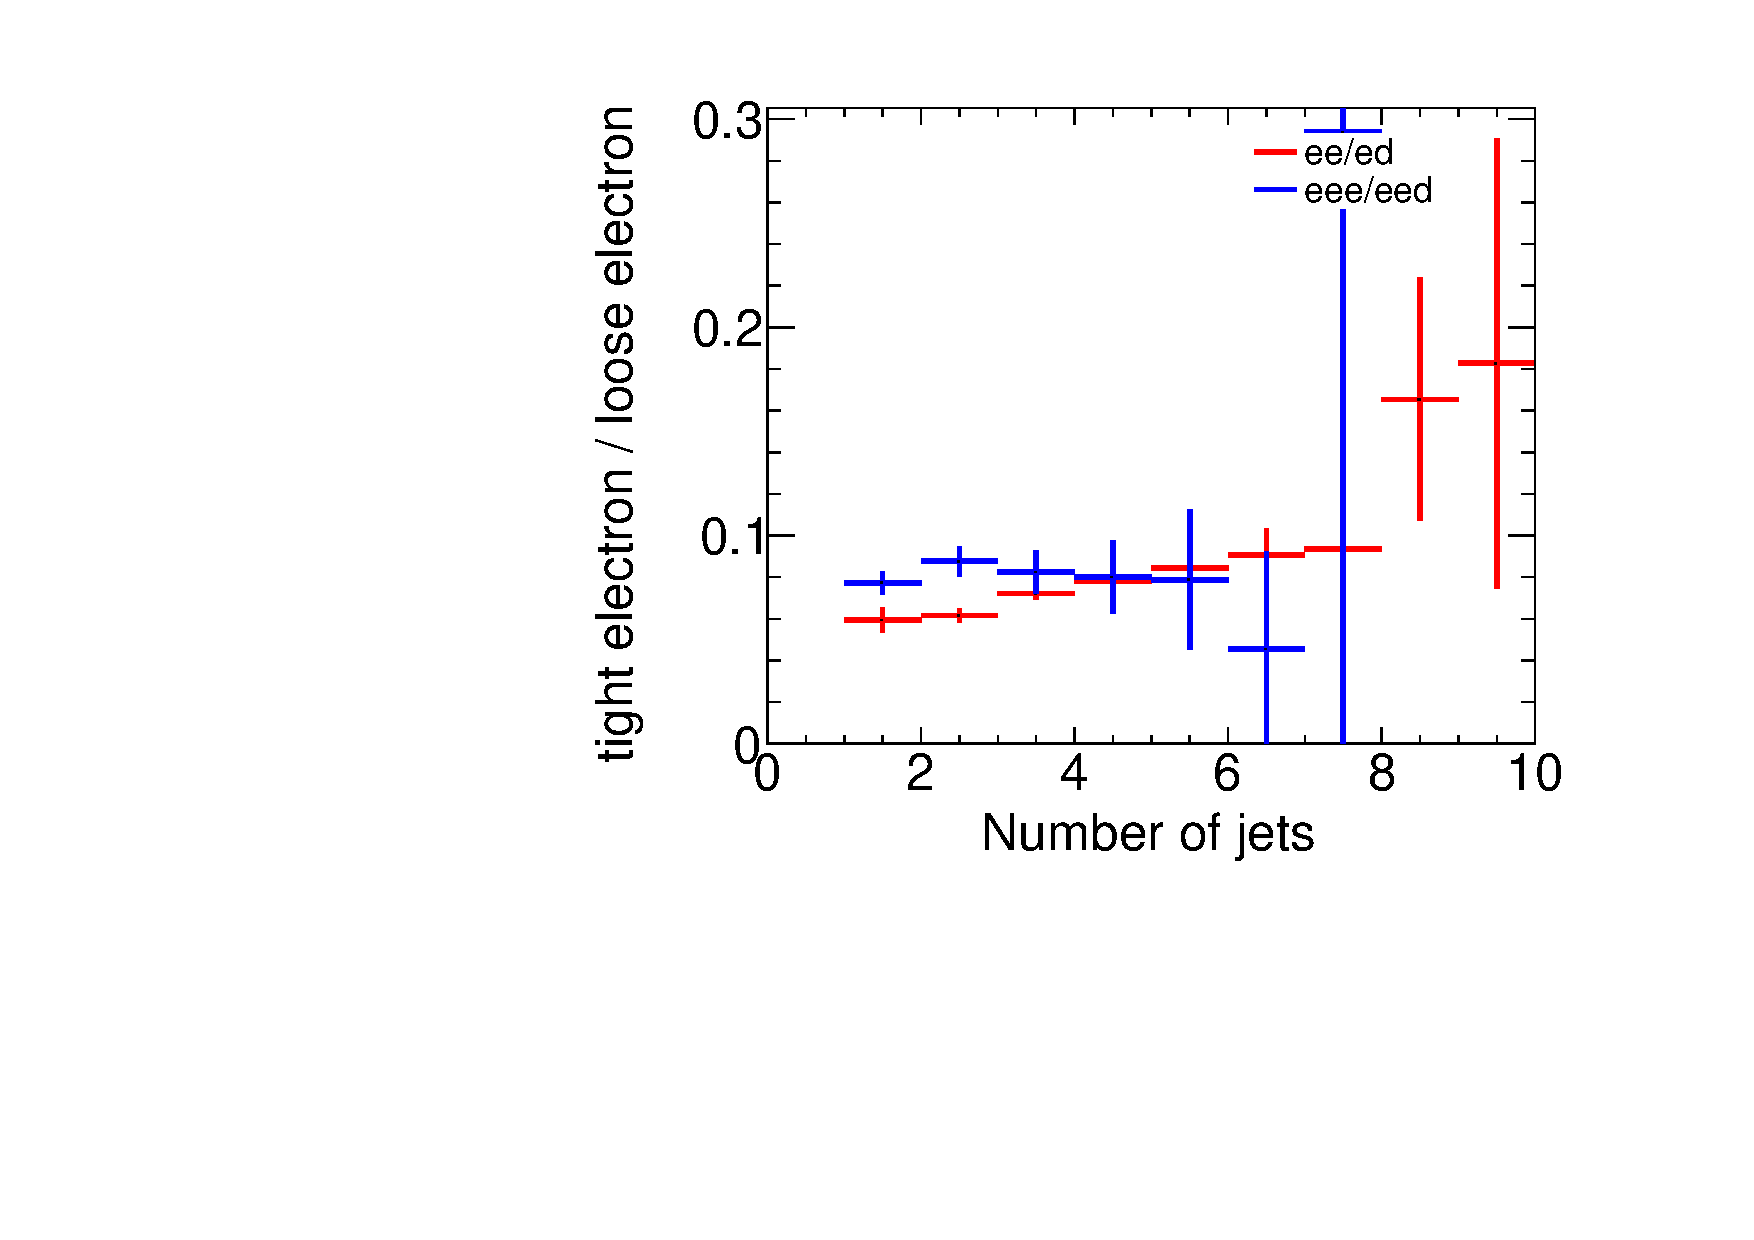
\includegraphics[width=\textwidth]{figs/fake/compare_2e_3e_NJet_ratios}
\end{minipage}\hfill
\begin{minipage}[h]{0.5\textwidth}
    \centering 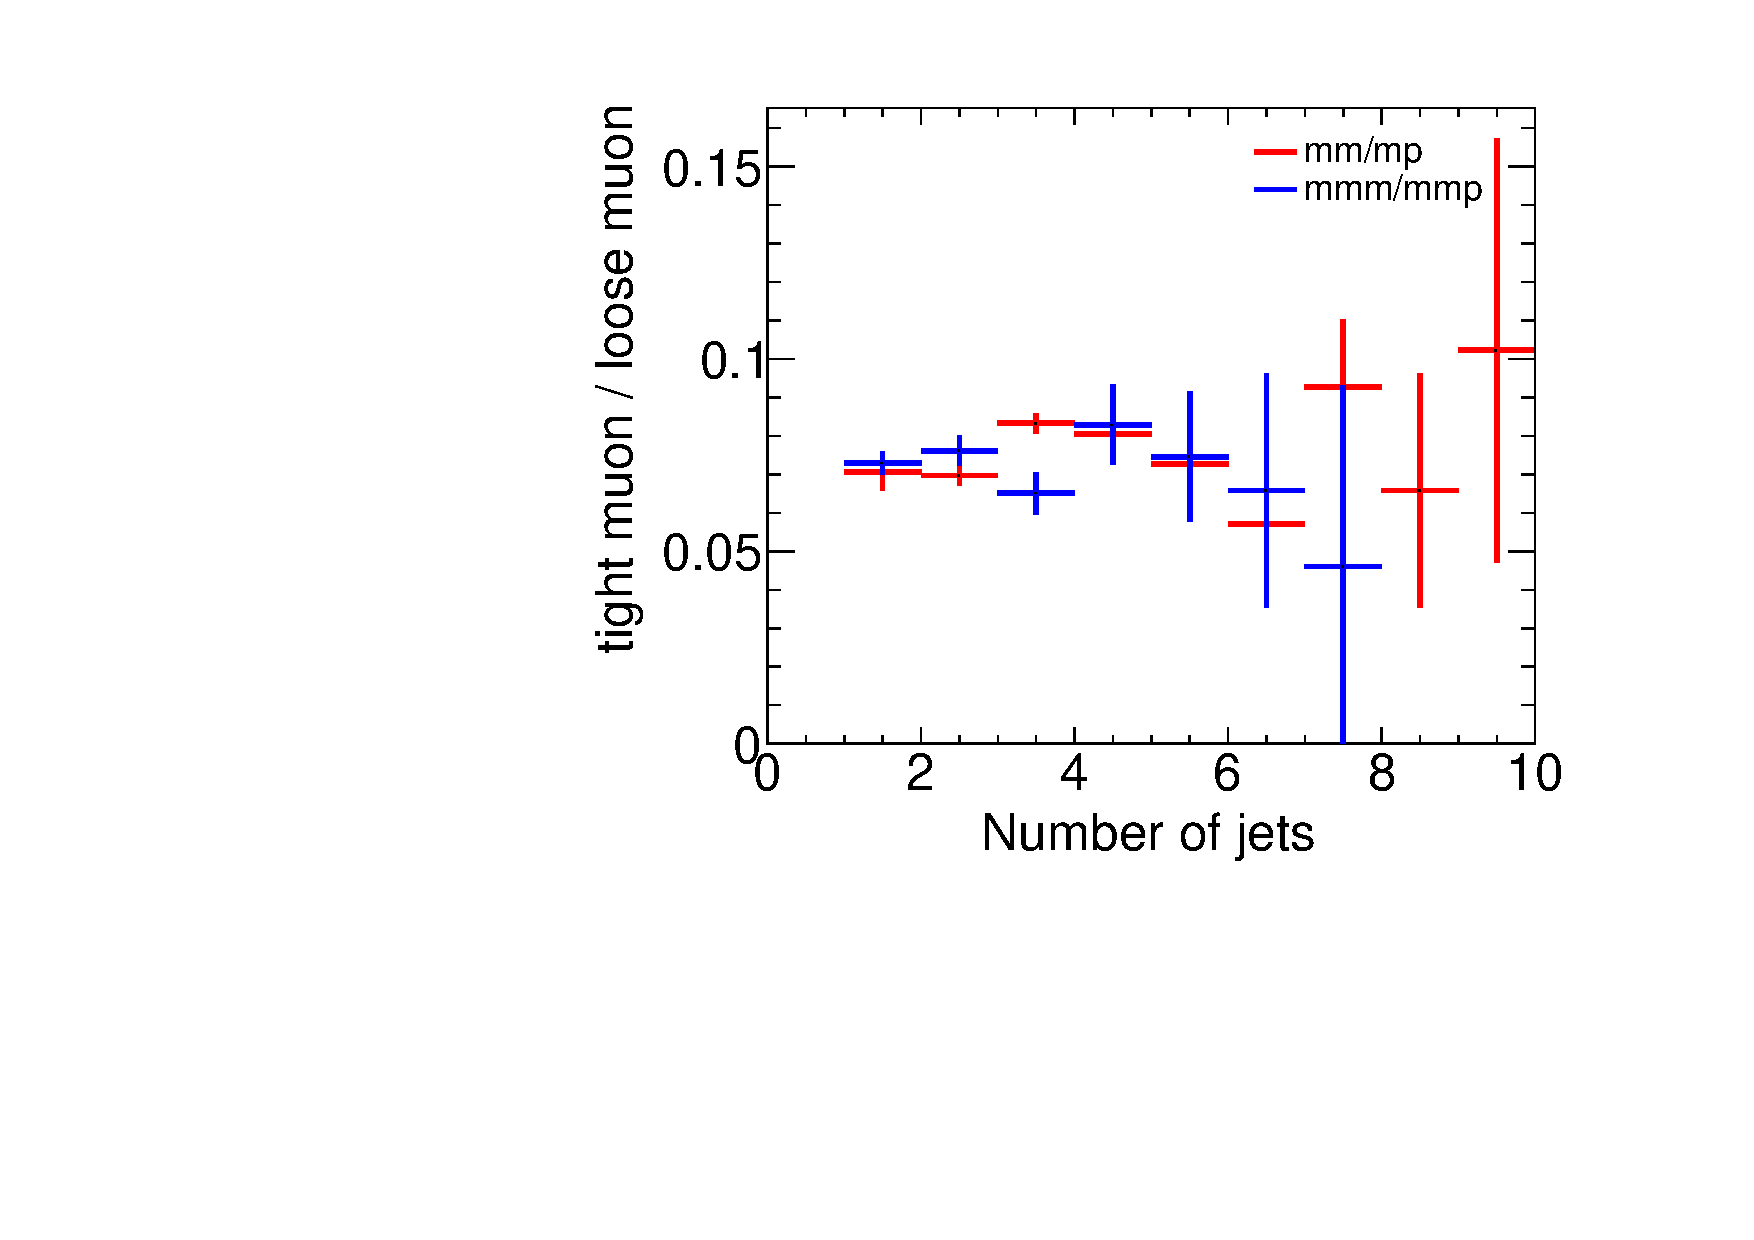
\includegraphics[width=\textwidth]{figs/fake/compare_2m_3m_NJet_ratios}
\end{minipage}\hfill
\caption{Ratios of regions with tight and anti-tight leptons in 2-lepton and 3-lepton channels from \ttbar\ MC. These ratios are the MC calculated transfer factors for each region, i.e. $\theta_e$ = $eee/eed$, $ee/ed$ and $\theta_{\mu}$ =$mmp/mmm$, $mm/mp$, where 'd' refers to anti-tight electrons and 'p' referes to anti-tight muons. The transfer factors are seen to be similar in the 2$\ell$ and 3$\ell$ cases and stable as a function of the number of jets}
\label{figure:background_njetr}
\end{figure}

Because these methods do not provide a per-object transfer-factor that depends on the properties of the faking object, we must use the MC to model the shapes of the fake kinematic distributions in the signal regions. This is not an essential issue, since the analysis only considers only the total number of events in each signal region in the final measurement of \tth\ production.

\subsection{2$\ell$ SS Fakes}
The 2$\ell$ SS fake method follows the procedure outlined in general above. We define anti-tight electron and muon control regions with reversed particle identification criteria for each signal region, including the 6 flavor and jet-counting sub regions. The anti-tight muon and electron criteria are provided below:
  
\begin{itemize}

\item \textbf{anti-tight electron (d):} fails the {\textsc verytight} likelihood operating point, but still passes the {\textsc veryloose} operating point. fails relative tracking and calorimeter isolation, $\rm E_{T}^{rel}>0.05$ and $\rm p_{T}^{rel}>0.05$.

\item \textbf{anti-tight muon (p):} 6 GeV $<$ \pt\ $<$ 10 GeV

\end{itemize}

The electron and muon transfer factors, $\theta_e$ and $\theta_{\mu}$, are calculated in the region with signal region selection but fewer jets, $NJet == 2$ or $NJet ==3$ and are defined as the ratio of the number of events for two fully identified leptons to the number of events with one fully identified lepton and one anti-identified lepton, after the prompt and charge misidentification backgrounds are subtracted. Only same-flavor channels are used to ensure that muon and electron transfer factors maybe estimated separately:
on every region, the prompt and charge-misidentification backgrounds are subtracted from the data. 

 \begin{equation}
 \theta_{e} = \frac{N_{ee}}{N_{ed}}= \frac{  N^{Data}_{ee} - N^{\rm
 Prompt~SS}_{ee} - N^{\rm QMisId}_{ee} }{ N_{ed}^{Data} - N^{\rm
 Prompt~SS}_{ed} - N^{\rm QMisId~MC}_{ed} } 
\end{equation}
\label{equation:ss_def_thee}


 \begin{equation}
 \theta_{\mu} = \frac{N_{\mu\mu}}{N_{\mu p}}= \frac{ N_{\mu\mu}^{Data} - N^{\rm
 Prompt~SS}_{\mu\mu}}{ N_{\mu p}^{Data} - N^{\rm
 Prompt~SS}_{\mu p} } 
\end{equation}
\label{equation:ss_def_thmm}

The 2,3 jet anti-tight regions used in obtaining the transfer factors are shown in Table~\ref{table:background_23jets} and the 4,5 jet
anti-tight regions, scaled by the transfer factors to get the fake estimates in the SR are shown in Figure \ref{figure:background_45jets}. 
The \ttbar\ and single top MC are included in the plots and tables for reference, although they are not used in the measurements. 

\begin{table}
  \begin{center}
\begin{tabular}{ c c }%% structure globale

\begin{tabular}{|c|c|}
\hline Process & N(events) \\ \hline
\multicolumn{2}{|c|}{$ed$ $\le 3$ jets} \\ \hline
$VV$  &    $7.13\pm0.63$ \\
$V\gamma$  &  $7.55\pm1.27$ \\
$t\bar{t}V, tV$     &    $6.68\pm0.18$ \\\hline
$V+jets$     &    $59.4\pm18.51$ \\
$t\bar{t},t+X$ &    $671.26\pm12.76$ \\
~$t\bar{t}$ prompts &    $32.97\pm 2.83$ \\\hline
Total MC & $752.0\pm22.5$ \\
Data & $967$ \\ 
Data fakes (Data - prompts) & $912.66$ \\ \hline\hline

\multicolumn{2}{|c|}{$ee$ $\le 3$ jets} \\ \hline
$VV$  &    $3.30\pm0.42$ \\
$V\gamma$  &  $1.31\pm0.65$ \\
$t\bar{t}V, tV$     &    $3.96\pm0.16$ \\\hline
$V+jets$     &    $8.3\pm8.8$ \\
$t\bar{t},t+X$ &    $11.65\pm1.67$ \\ \hline
Charge misID &    $ 8.54 \pm 0.23 $ \\\hline
Total MC & $28.52 \pm 8.96$  \\
Data & $32$ \\ \hline
Data fakes (Data - prompts) & $14.26$ \\ \hline\hline

\end{tabular}

&


\begin{tabular}{|c|c|}
\hline Process & N(events) \\ \hline

\multicolumn{2}{|c|}{$\mu p$ $\le 3$ jets} \\ \hline
%\multicolumn{2}{|c|}{Prompts Same-Sign} \\ 
$VV$  &    $4.34\pm0.44$ \\
$V\gamma$  &  $4.84\pm2.05$ \\
$t\bar{t}V, tV$     &    $0.74\pm0.06$ \\\hline
$V+jets$     &    $21.77\pm12.24$ \\
$t\bar{t},t+X$ &    $192.71\pm6.59$ \\\hline
Total MC & $224.4 \pm 14.1$ \\ 
Data & 249 \\
Data fakes (Data - prompts) & $239.07$ \\ \hline\hline

\multicolumn{2}{|c|}{$\mu\mu$ $\le 3$ jets} \\ \hline
%\multicolumn{2}{|c|}{Prompts Same-Sign} \\ 
$VV$  &    $6.27\pm0.56$ \\
$V\gamma$  &  $0.06\pm0.25$ \\
$t\bar{t}V, tV$ &    $10.00\pm0.27$ \\\hline
$V+jets$     &    $ 1.22 \pm 11.78$ \\ %% huge number of samples with 0 evts %% -> neglected
$t\bar{t},t+X$ &    $15.4\pm2.1$ \\\hline
Total MC & $32.95 \pm 2.21$ \\ 
Data & 44 \\ 
Data fakes (Data - prompts) & $27.65$ \\ \hline\hline

\end{tabular}


 \end{tabular}
\caption{Number of events of the main simulated background processes and of
  the data in the \ee and \mumu channels used for the measurement of
  $\theta_e$ and $\theta_\mu$. $VV$, $V\gamma$, $t\bar{t}V, tV$ and $t\bar{t}$~prompts
  (or charge misID) are the backgrounds which lead to prompt same-sign dileptons and are subtracted from
  the data to get a measured number of fakes. Uncertainties are
  statistical. The numbers labeled Data fakes are used to
  measure $\theta$. 
  \label{table:background_23jets}} 
\end{center} \end{table}
 




  % Figures
 \begin{figure}[htbp]

  \begin{minipage}[h]{0.5\textwidth}
    \centering 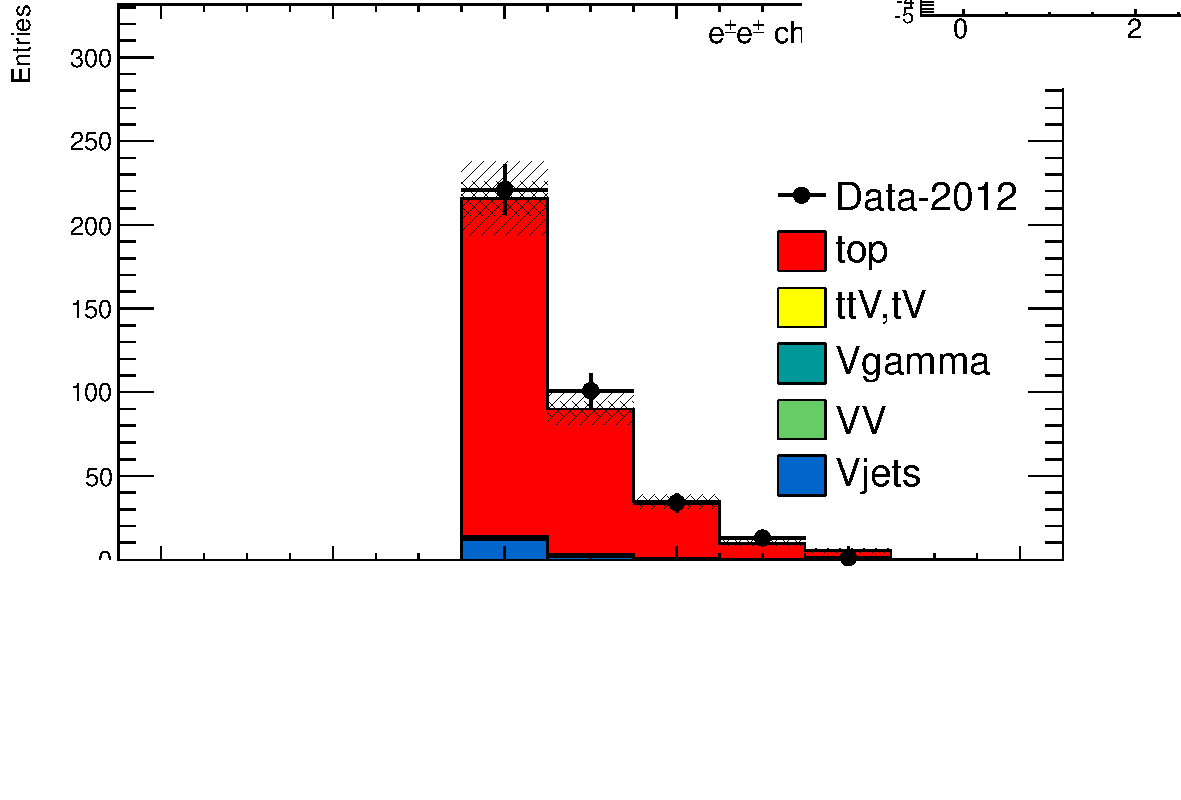
\includegraphics[width=\textwidth]{figs/fake/TaT-5jets-1b_nj_ee}
  \end{minipage}\hfill
  \begin{minipage}[h]{0.5\textwidth}
    \centering \includegraphics[width=\textwidth]{figs/fake/TaT-5jets-1b_nb_ee}
  \end{minipage}\hfill
  \begin{minipage}[h]{0.5\textwidth}
    \centering \includegraphics[width=\textwidth]{figs/fake/TaT-5jets-1b_nj_mm}
  \end{minipage}\hfill
  \begin{minipage}[h]{0.5\textwidth}
    \centering \includegraphics[width=\textwidth]{figs/fake/TaT-5jets-1b_nb_mm}
  \end{minipage}\hfill

  \caption{4,5 Jet SS 2$\ell$  $ed$ (above) and $\mu p$ control regions with at least one b-tagged jet. After subtraction of prompt and charge misidentification backgrounds, these regions
    are scaled by the transfer factors, $\theta_e$ and $\theta_{\mu}$, to obtain the final number of fake events in the CR. The top MC (red) is
  used for reference but not in the actual calculation.}
  \label{figure:background_45jets}
 \end{figure}

The transfer factors obtained from the 2 and 3 jet regions are shown in \ref{table:background_theta} with statistical errors and propagated systematic
errors from the subtraction of relevant backgrounds (\ttV\ and charge misidentification). The MC values are just for comparison. An additional 
systematic error is added by comparing the transfer factors, obtained from the low jet control region, to those obtained from the 
higher jet signal regions, using \ttbar\ MC. The value of this systematic is about 20 \% and can be seen in the above Figure \ref{figure:background_njetr}.
The overall systematic uncertainties and contribution from each source in all of the sub-channels of the signal region are shown in Table \ref{table:background_theta}
and the final contribution of fake events to the signal region are show in Table \ref{table:background_summary} found at the beginning of the chapter.  

\begin{table}
  \begin{center} 
{\small \begin{tabular}{ l c c }
\hline Factor    &  Expected (MC) & Measured (data) \\ \hline
 $\theta_{e}$ Rev. Id.  & $0.0136\pm 0.0062$  & \textit{ 0.0156$\pm$0.0062}  \\ 
 $\theta_{\mu}$ Rev. $p_{\rm T}$ & $0.078\pm0.012$ & \textit{ 0.1156$\pm$0.0288} \\ \hline %% Mc here is based full top

\end{tabular}}
\caption{ Expected and measured values of the $\theta$ factors. NEEDS TO BE UPDATED FOR 2,3\label{table:background_theta}} 
\end{center}
\end{table} 
 % Errors 


\begin{table}[h!]
  \begin{center} 
{\small \begin{tabular}{|l|l|ccc|ccc|}
\hline \multicolumn{2}{|c|}{ } &  \multicolumn{6}{c|}{Channels} \\ \cline{3-8}
 \multicolumn{2}{|c|}{Uncertainties} &  \multicolumn{3}{c|}{$4$ jets} &  \multicolumn{3}{|c|}{$\ge 5$ jets} \\ \cline{3-8}
\multicolumn{2}{|c|}{} & $e^{\pm}e^{\pm}$ & $\mu^{\pm}\mu^{\pm}$ & $e^{\pm}\mu^{\pm}$ & $e^{\pm}e^{\pm}$ & $\mu^{\pm}\mu^{\pm}$ & $e^{\pm}\mu^{\pm}$  \\ \hline\hline

    &  $\Delta\theta_{e}^{\rm stat}$ & 39.6 & -- & 14.2 & 39.6 & -- & 18.5 \\ \cline{2-8}
   Statistical    &  $\Delta\theta_{\mu}^{\rm stat}$ & -- & 24.7 & 15.8 & -- & 24.7 & 13.1 \\ \cline{2-8}
    &  $\Delta N_{\ell anti-\ell}(n~ {\rm jets})$(stat) & 6.8 & 18.1 & 21.3 & 8.4 & 25.9 & 22.7 \\ \hline

    &  $\Delta\theta_{e}^{\rm syst}$ (closure) & 21.8 & -- & 7.8 & 26.7 & -- & 12.5 \\ \cline{2-8}
Systematics    &  $\Delta\theta_{\mu}^{\rm syst}$ (closure) & -- & 23.3 & 18.4 & -- & 31.2 & 19.7 \\ \cline{2-8}
    & Q Mis Id ($\ell anti-\ell$) & 2.2 & -- & 1.5 & 2.4 & -- & 1.5 \\ \hline

\multicolumn{2}{|c|}{Total} &\bf 45.7 &\bf 38.5 (36.3) &\bf 35.7 &\bf 48.5 &\bf 47.8 (43.9) &\bf 39.6 \\ \hline
Systematic    & Q Mis Id ($\ell\ell$) & 24.0 & -- & 8.6 & 24.0 & -- & 11.3 \\ \hline
\hline \end{tabular}}
\caption{ Summary of the uncertainties (in \%) in \ee (reverse Id + reverse isolation
  method), \mumu and \emu. Statistical uncertainty is split into statistical
  uncertainties on $\theta_{e}$ and $\theta_{\mu}$ and uncertainty due to the
  Control Region size ($\Delta N_{\ell anti-{\ell}}(n~ {\rm jets})$). For channels with muons, uncertainties
  between parenthesis are obtained when anti-tight muons are defined such as
  $p_{\rm T}<20$~GeV (includes blinded data) \label{tab:uncertainties}}
\end{center}  
 \end{table}


  % Needs to be updated by Djamel




\subsection{3$\ell$ Fakes}

The 3$\ell$ fake method follows the same general strategy as the 2$\ell$ SS case. Transfer factors are used to extrapolate from anti-tight, fake-rich control regions in data  into the signal region.  However, the equivalent low jet control regions are too low in statistics to provide the transfer factors from data directly. Instead, the transfer factors are obtained directly from the \ttbar\ simulation. Data control regions, called auxiliary regions, are used to determine the modeling of the identification and isolation variables, used in the transfer factor extrapolation. The low jet regions are still employed in a low statistics validation of the entire fake procedure. 

Anti-tight electrons and muons are defined in slightly different ways, compared to the 2$\ell$ SS case:
\begin{itemize}
\item \textbf{ anti-tight electron (d):} fails to pass the {\textsc verytight} likelihood operating point, but still verifies the {\textsc veryloose} operating point. The isolation selection is released $\rm E_{T}^{rel}>0.05$,  $\rm p_{T}^{rel}>0.05$.

\item \textbf{ anti-tight muon (p):} muons must pass identification but the \pt\ cuts is lowered to 6 GeV. The overlap removal with jets and isolation cuts are released.
\end{itemize} 
The transfer factors, $\theta_e$ and $\theta_{\mu}$, extracted from MC, is defined as the ratio of the number of top (\ttbar\ + single-top) events in the signal region, to the number of \ttbar\ events in the anti-tight regions. The factors are calculated in separate flavor regions to ensure that the electron jet fakes and muon jet fakes are calculated separately. The calculation follows the same form as for the 2$\ell$ SS case, but now lep0, which by construction is almost never a fake is allowed to be either electron or muon in both cases, denoted below in Equations \ref{equation:background_theta_3l_e} and \ref{equation:background_theta_3l_m}.  

\begin{equation}
\theta_e = \frac{N^{top}_{xee}}{N^{top}_{xed}}
\label{equation:background_theta_3l_e}
\end{equation}

\begin{equation}
\theta_{\mu} = \frac{N^{top}_{x\mu\mu}}{N^{top}_{x\mu p}}
\label{equation:background_theta_3l_m}
\end{equation}




The MC modeling of the variables involved in the transfer factor can be verified when another variable fails. For instance, the MC modeling of the electron isolation variable can be compared to data when the particle identification variable fails and vice-versa. The modeling of muon-jet $\Delta R$, involved in the overlap removal, can be compared when either the isolation variable or the \pt\ fails. The comparison of the electron variables in this manner can be seen in Figure \ref{figure:background_electron_dataMC} and the muon variables in Figure \ref{figure:background_muon_dataMC}. The regions used have the same selection as the signal region with an added missing transverse energy requirement, $>$ 60 GeV, to ensure only top fakes. 20\% and 30\% systematic uncertainties are assigned to the muon and electron transfer factors, respectively, to account for data-MC discrepancies. This method for evaluating data-MC agreement for individual electron and muon variables in turn relies on the assumption that these variables are largely uncorrelated and that the transfer factor itself is factorizable into pieces for each variable. Factorized and fully correlated transfer factors have been compared using MC and shown to have differences smaller than the systematic quoted, suggesting that the uncorrelated assumption is reasonable. 


\begin{figure}[!htbp]
  \begin{minipage}[h]{0.5\textwidth}
    \centering \includegraphics[width=\textwidth]{figs/fake/h_muPt_CR_early_AF2_extrap_MET50_noIso_RESCALED}
  \end{minipage}\hfill
  \begin{minipage}[h]{0.5\textwidth}
    \centering \includegraphics[width=\textwidth]{figs/fake/h_minDRjet_CR_early_AF2_extrap_MET50_noIso_RESCALED}
  \end{minipage}\hfill
  \begin{minipage}[h]{0.5\textwidth}
    \centering \includegraphics[width=\textwidth]{figs/fake/h_relptcone20_CR_early_AF2_extrap_MET50_noIso_RESCALED}
  \end{minipage}\hfill
  \begin{minipage}[h]{0.5\textwidth}
    \centering \includegraphics[width=\textwidth]{figs/fake/h_reletcone20_CR_early_AF2_extrap_MET50_noIso_RESCALED}
  \end{minipage}\hfill
  \caption{Distributions of the properties of the anti-tight muons in data (dots), compared with the total simulation (red line), rescaled to the integral of the data for a shape comparison. The uncertainty on the data distribution is statistical. The number of events for each of them is also presented in the legend. The variables probed are, top: $p_T$ and $\Delta R(\mu, {\rm , closest \, selected \, jet})$; bottom: ptcone20/$p_T$ and Etcone20/$p_T$. The selection is the signal region event selection with one anti-tight muon (failing at least one of the isolation, muon-jet overlap, or \pt\ selection criteria). A ratio plot is containing the $20\%$ area around 1, is displayed, demonstrating that a 20\% data-MC comparison systematic is sufficient.}
  \label{figure:background_muon_dataMC}
\end{figure} 


\begin{figure}[!htbp]
  \begin{minipage}[h]{0.5\textwidth}
    \centering \includegraphics[width=\textwidth]{figs/fake/aux_d2_Obj0VeryTightLH}
  \end{minipage}\hfill
  \begin{minipage}[h]{0.5\textwidth}
    \centering \includegraphics[width=\textwidth]{figs/fake/aux_d1_Obj0PtIso20Rel}
  \end{minipage}\hfill
  \begin{minipage}[h]{0.5\textwidth}
    \centering \includegraphics[width=\textwidth]{figs/fake/aux_d1_Obj0EtIso20Rel}
  \end{minipage}\hfill
  \caption{Distributions of anti-tight electron variables. The variables presented are, from top left to bottom right, $p_T$, $\eta$, \textsc{verytight} Likelihood value, ptcone20/$p_T$, Etcone20/$p_T$. The plotted regions have the same cuts as the signal region, except the anti-tight electron must fail isolation for the plot of the \textsc{verytight} identification word or fail the \textsc{verytight} identification word for the plots of the isolation. Data (dots) are compared with a stacked histogram of the various simulated samples: top in red, $V$+jets (blue), $VV$ (purple) and \ttV\ (yellow). The uncertainty on the data distribution is statistical. }   
  \label{figure:background_electron_dataMC}
\end{figure} 
%

The electron and muon anti-tight control regions, which are scaled by the transfer factors are shown in Figure \ref{figure:background_3lcr}. The prompt MC subtracted data in these regions are scaled by the transfer factors to obtain the overall contribution of fake electron and muon events in the signal region. The systematic uncertainties are split between the statistical error on the transfer factor and normalization of the anti-tight control regions and the data-MC comparisons outlined above. For muon fakes the total systematic uncertainty is 25\% and for electrons it is 34\%. The numbers and uncertainties involved in the calculation are shown in Table \ref{table:background_3l_summary}.  


\begin{figure}[!htbp]
  \begin{minipage}[h]{0.5\textwidth}
    \centering \includegraphics[width=\textwidth]{figs/fake/h_nBtags_CR_AF2_fakesCR1_noOR}
  \end{minipage}\hfill
  \begin{minipage}[h]{0.5\textwidth}
    \centering \includegraphics[width=\textwidth]{figs/fake/h_nJets_CR_AF2_fakesCR1_noOR}
  \end{minipage}\hfill
  \begin{minipage}[h]{0.5\textwidth}
    \centering \includegraphics[width=\textwidth]{figs/fake/cr_d1_NJet}
  \end{minipage}\hfill
  \begin{minipage}[h]{0.5\textwidth}
    \centering \includegraphics[width=\textwidth]{figs/fake/cr_d1_NJetBTag}
  \end{minipage}\hfill

  
  \caption{Muon-xxp (above) and electron-xxd (below) anti-tight control regions: jet variables. Note: the \ttbar\ and single top MC in the plots is used only as comparison, but is not included
  in the fake measurement}
  \label{figure:background_3lcr}
  \end{figure} 

\begin{table}[!htbp]
\begin{center} 
\begin{tabular}{|c|c|c|} 
  \hline
  Stage   & Muon & Electron \\
  \hline
  Anti-Tight CR Normalization  &  364.62 $\pm$ 20.02 (5$\%$) & 38.2 $\pm$ 6.9 (17\%) \\ 
  \hline  
  Transfer factor  & $0.0047 \pm 0.0011$ (23$\%$) & 0.0240 $\pm$ 0.0064 (36\%) \\
  SR Contribution & 1.71 $\pm$ 0.42 (25\%)           & 0.91 $\pm$ 0.35(39\%) \\ 
  \hline  
\end{tabular}
\caption{Summary of regions and inputs to the extraction of the number of \ttbar\ events with a fake muon in the SR}
\label{table:background_3l_summary}
\end{center}
\end{table}


The low jet region (1, 2, 3) is used as a validation for the method. The \ttbar\ and single top fakes in this region are estimated using the procedure above. Similar systematics are assessed. This region with the fake estimate is plotted in Figure \ref{figure:background_3lvaldiation}. The agreement of data and summed prediction for the fakes and prompt backgrounds is well within the systematic and statistical uncertainties. The figure also shows the same region with relaxed \pt\ cuts on all leptons to 10 GeV, which enriches the fake contributions greatly.   The data and summed fake and prompt predictions are also well within the statistical and systematic uncertainties.


\begin{figure}[!htbp]
  \begin{minipage}[h]{0.5\textwidth}
    \centering \includegraphics[width=\textwidth]{figs/fake/plotCand_3lep_C_NJet}
  \end{minipage}\hfill
  \begin{minipage}[h]{0.5\textwidth}
    \centering \includegraphics[width=\textwidth]{figs/fake/plotCand_3lep_C_NElec}
  \end{minipage}\hfill
  \begin{minipage}[h]{0.5\textwidth}
    \centering \includegraphics[width=\textwidth]{figs/fake/plotCand_3lep_LowNJet_NJet}
  \end{minipage}\hfill
  \begin{minipage}[h]{0.5\textwidth}
    \centering \includegraphics[width=\textwidth]{figs/fake/plotCand_3lep_LowNJet_NElec}
  \end{minipage}\hfill
  \caption{ 3$\ell$ fake validation regions for nominal \pt\ selection (above) and relaxed \pt\ selection, $>$ 10 GeV, (below). Plotted are the number of jets and the number of electrons in each event. The data and MC ratio below each plot agree with 1 within the statistics of the region and the overall systematic assigned for the fake component (red)}  
  \label{figure:background_3lvaldiation}
\end{figure} 



\subsection{4$\ell$ Fakes}

We will not discuss the 4$\ell$ fakes in depth, as it is a very small background - at the \% level and will have almost no impact on the final result. The fake method used in the the 4$\ell$ case is similar to the 2$\ell$ and 3$\ell$ cases discussed above. All fakes arise from \ttbar\ and single-top events, where \textit{two} jets are misidentified as leptons. To measure the contribution of this background, control regions with 2 fully identified and 2 anti-identified leptons are created. These control regions do not have a number of jets requirement in order to increase statistics.  From these control regions, two extrapolations are made. First, a transfer factor is applied to extrapolate from the anti-tight to tight regions for electrons and muons. The regions are defined with identical object identification selection and reversal as the 3$\ell$ case, and the same transfer factors can be used. They must be used twice however, because there are two anti-identified leptons in each event. Second, the jet inclusive regions are extrapolated into the 2-jet signal region, using a second extrapolation factor derived from \ttbar\ events. Since, the majority of fake leptons arise from b-quark initiated jets, the jet spectrum \ttbar\ events with the additional requirement of 2-b-tagged jets from data are used as a model for the jet extrapolation. The overall systematic uncertainty on this measurement arises from the statistics in the control regions and MC based assessments of non-closure and are 35\%-50\% depending on the sub-channel. 



\chapter[Summary of Systematic Uncertainties][Summary of Systematic Uncertainties]{Summary of Systematic Uncertainties}
\label{chapter:systematics} 

This chapter summarizes the systematic uncertainties that enter the measurement of the limit of \tth\ multi-lepton analysis. The systematic uncertainties arise from three main sources. The first are the normalization uncertainties on the background process estimation methods, which are discussed in depth in Chapter~\ref{chapter:background}. The second source is the theoretical uncertainties on the \tth\ production cross-section and acceptance. The final source are the experimental and detector related systematic uncertainties related to event selection efficiencies and measurements and identification of the objects. They affect only the non-data driven backgrounds and the \tth\ signal, as simulation is used to model their acceptance and efficiency for the analysis selection. 

These systematic uncertainties, the estimated background and signal event counts in each of the signal regions, and the observed data in each signal region are combined in a statistical fit to an analysis model to extract the measurement of interest. We measure per-channel and combined ratios of the observed production rate to the theoretically predicted production rate of \tth, a parameter called $\mu$. In the absence of a statistically significant observation, this measurement is translated into a upper confidence limit
on $\mu$. The details of this procedure are discussed in the following sections and the results with the observed data are discussed in Chapter \ref{chapter:results}

\section{Systematic Uncertainties on Signal Cross-section and Acceptance}
\label{section:tth}
The \tth\ signal is simulated with matrix elements at NLO in QCD with {\textsc Powhel}. The simulation details are discussed in Chapter \ref{chapter:data}. The production cross section and the Higgs boson decay branching fractions together with their theoretical uncertainties from the QCD scale and PDF choice are taken from the NLO theoretical calculations reported in \cite{Heinemeyer:2013tqa}. The uncertainty from the QCD scale estimated by varying $\mu_{0}$ by a factor of 2 from the nominal value is $^{+3.8\%}_{-9.3\%}$, while the uncertainty from the PDF set and the value of $\alpha_{\rm S}$ is $\pm 8.1\%$.

The impact of the choice of the QCD scale on the simulation of the \ttbar$H$ event selection efficiency is estimated in two independent ways. 

First, the factorization and renormalisation scales $\mu_{0}$ are varied by a factor of 2, as $\mu = 2\mu_{0}$ and $\mu = \mu_{0}/2$. The effects of these new scales are estimated via the application of event re-weighting procedures on the nominal simulation using kinematic distributions at parton level. The weights used are dependent on the transverse momenta of both the \ttbar$H$ system and of the top quark, as described in \cite{Guindon:1638000}. 

Second, the choice of the factorization and renormalisation scales, dependent on fixed (static) parameters in the nominal simulation, is tested comparing its prediction with an alternative (dynamic), but still physics motivated choice $\mu_{0} = (m_{T}^{t}m_{T}^{\bar{t}}m_{T}^{H})^{\frac{1}{3}}$, which depends on kinematic variables. This comparison is performed via event re-weighting of the nominal static simulation based on weights derived as a function of the \ttbar$H$ transverse momentum~\cite{Guindon:1638000}. In order to take the difference between the choices of scale as systematic uncertainties, a symmetric envelope around the nominal simulation is built applying the weights and also their inverses.

In order to not double-count the variations on the total cross section the predictions from the different QCD scales are normalized to the same total cross section. That means that the observed differences are only coming from the event selection.
Significant variations on the jet multiplicities can be seen and these translate into different predictions on the signal event yields in the signal regions. Such differences, listed in Table~\ref{table:systematics_theosystttH}, are taken as theoretical systematic uncertainties in addition to the ones affecting the total \ttbar$H$ production cross section. The static uncertainties come from the variations by a factor of 2 from the nominal scale and they are correlated with the uncertainties on the total cross section, which are estimated with the same procedure. The dynamic uncertainties come from the difference between the nominal and the alternative dynamic scale and are treated as an independent source of theoretical uncertainty. 

\begin{table}
\caption{Theoretical uncertainties of the signal event yields in the signal regions due to the impact of QCD scale uncertainties on the event selection.}
\begin{center} 
\begin{tabular}{r|c|c|c|c|}
QCD scale [\%] & 2$\ell$4jets & 2$\ell$$\geq$5jets & 3$\ell$ & 4$\ell$ \\
\hline
Static   & $^{+0.6}_{-0.0}$ & $^{+2.7}_{-1.3}$ & $^{+2.3}_{-0.8}$ & $^{+0.9}_{-0.2}$ \\
Dynamic  & $^{+1.7}_{-0.8}$ & $^{+2.0}_{-2.6}$ & $^{+1.7}_{-1.1}$ & $^{+0.5}_{-0.0}$ \\
\hline
\end{tabular}
\end{center}
\label{table:systematics_theosystttH}
\end{table}%

The uncertainty of the \ttbar$H$ event selection due to the PDF sets is estimated comparing the predictions with three different PDF sets, varying each set within errors and taking the width of the envelope as systematic uncertainty. The recommended sets are \verb+CT10+, \verb+MSTW2008nlo68cl+ and \verb+NNPDF21_100+. 

Figure~\ref{figure:systematics_theosystPDF} shows the estimated PDF systematic uncertainties as a function of the jet multiplicity in \ttbar$H$ events with at least two leptons. The uncertainties are compatible with the uncertainty on the production cross section estimated in \cite{Heinemeyer:2013tqa} and indicated by the dashed red lines in the lower panel. 
Table \ref{table:systematics_pdfaccttH} shows the half-width of the envelope of the acceptance under all eigenvector variations of the three PDF sets.
No significant dependence on the event topology is observed, so that the PDF systematic uncertainty on the \ttbar$H$ event selection is neglected.
\begin{figure}[htbp]
\begin{center}
\includegraphics[width=0.6\textwidth]{figs/tth/plot_PowhegPythia8_AU2CT10_PowHelttH120inc_ljets_AFII_njets_all_njets_all}
\caption{PDF systematic uncertainty on the jet multiplicities in \ttbar$H$ events with at least 2 leptons. The dashed red lines in the lower panel indicate the systematic uncertainty on the \ttbar$H$ production cross section.}
\label{figure:systematics_theosystPDF}
\end{center}
\end{figure}

\begin{table}
\begin{center}
\caption{\label{table:systematics_pdfaccttH}Uncertainties on $\ttbar H$ acceptance in signal
  regions due to PDF variation.}
\begin{tabular}{r|c|c|c|c}
Sample & 2$\ell$ 4j & 2$\ell$ 5j & 3$\ell$ & 4$\ell$\\
\hline
$\ttbar H$ & 0.3\% & 1.0\% & 0.5\% & 1.4\%\\
\end{tabular}
\end{center}
\end{table}



\section{Experimental and Detector Systematic Uncertainties}
 
Experimental and detector systematic uncertainties affect the efficiencies of identifying objects and the efficiencies for events to pass our cuts . These uncertaintites affect only MC models of physics processes, \ttV, \tth, $VV$ and thus alter ther number of expected events from signal and backgroun in our signal regions. Data-driven backgrounds take into account these uncertainties by construction. We consider systematic effects from a number of sources: the lepton and jet energy scale measurements, the lepton identification and isolation selections, the efficiency and misidentification rate associated with tagging b-quark jets. Effects due to modeling the energy and objects from additional vertices were studied and found to be negligible. The vast majority of the individual detector systematics effects are small. The sum total of the systematic effects are comparable to the overall normalization and cross-section uncertainties on some of the physics processes and is shown in Table \ref{table:systematics_total_detector}.

\subsection{Lepton Identification, Energy Scale, and Trigger}
The electron\cite{ATLAS-CONF-2014-032} and muon identification efficiencies\cite{MuonSF} are measured in data using $Z$ boson and $J/\Psi$ control samples. They muon efficiencies are shown in Figure \ref{figure:systematics_lepidsf}, while the lectron efficienceis are shown in Figure~\ref{figure:electron_eff}. The uncertainty on the muon efficiencies are measured as functions of $\eta$ and \pt\ and are generally less 1\%. The uncertainty on the electron and muon efficiencies are also measured as functions of $\eta$ and \pt\ and are at the 1\% level for \pt\ above 30 GeV, but become much larger 5-10\% for the lower \pt\ regimes.   These translate into sub-1\% level effects on the \ttV\ and \tth\ event counts in the signal regions for the muons and 1\% level effects for the electrons. The effects become more important with increasing numbers of leptons.  

\begin{figure}[htbp]
\begin{center}
\includegraphics[width=0.60\textwidth]{figs/systematics/fig_18a}
\caption{Muon identification efficiency in Data and MC as a function of $\eta$. The CB+ST (combined+segment tagged) operating point is used}
\label{figure:systematics_lepidsf}
\end{center}
\end{figure}

The electron\cite{EgammaReco} and muon\cite{MuonSF} energy scale and resolution are also measured using the $Z$-boson control samples in data. The uncertainties related to the scale and resolution for the leptons affect the overall event acceptance through the lepton momentum cuts primary and have negligible impact on the event count uncertainties in the signal regions.

The efficiencies for muons and electrons to pass muon\cite{ATLAS-CONF-2012-099} and electron triggers\cite{ATLAS-CONF-2012-048} have been calculated with respect to the offline identification operating points using the $Z$ boson control samples. They are in the range of 90\% for electron triggers and 70\% for muon triggers, owing to gaps in muon trigger coverage, and have 1\% level uncertainties. When statistically combined for 2$\ell$ SS, 3$\ell$ and 4$\ell$ lepton signal regions, the overall trigger efficiency is high and the uncertainties on the number of expected events is negligible. 


\subsection{Lepton Isolation and Impact Parameter}

The isolation and impact parameter selections are specific to this analysis and are discussed in depth in Chapter \ref{chapter:selection}. We calculated their combined efficiency with respect to the full lepton identification selection using the $Z$ boson control samples and define data-MC scale factors to correct the efficiency in the simulation. Background are subtracted using shape templates in the di-lepton invariant mass spectrum. The $Z$-event template is derived from MC, while the background template is derived from the same-sign control region. We measure the efficiency scale-factors in bins of lepton momentum. Uncertainties are assigned per-bin to account for the level of statistics and variations caused by the fit parameters. An additional 1\% uncertainty envelope is added to both the electron and muon measurements to account for trends observed in the dependence of the data-MC efficiency scale-factor as a function of the number of jets. Stability of the efficiency scale-factor as a function of the number of jets is important for this analysis, because event activity in the low jet $Z$ sample, where the efficiency is measured, is much different from the high jet signal regions, where the efficiency is applied. The dependence of the scale-factor on the number of jets can be seen Figure \ref{figure:systematics_iso}. The isolation scale-factor uncertainties are around 1-3\% depending on the particle momentum, but these uncertainties propagate to 2-5 \% (some of the largest) effects in the event counts in the signal regions. The uncertainties are more important in the regions with more leptons. 


\begin{figure}[htbp]
\begin{center}
\includegraphics[width=0.48\textwidth]{figs/systematics/MuTP_sf_njet_ALP}
\includegraphics[width=0.48\textwidth]{figs/systematics/EleTP_sf_njet_ALP}
\caption{Muon (left) and electron(right) isolation efficiency scale-factors from the $Z$ control sample as a function of the number of jets in the event. An additional systematic uncertainty of 1\% is added to encompass the variation in the number of jets variable}
\label{figure:systematics_iso}
\end{center}
\end{figure}


\subsection{Jet Energy}

The jet energy scale (JES) is calculated using a combination of data-based in-situ techniques, where jet transverse momentum is balanced with respect to a reference photon or a Z boson, as well as single particle test-stand studies\cite{Aad:2014bia}. Additional smaller effects are taken into account including the b-quark jet specific response, near-by jets, the effects of pile-up and an inter-calibration of similar $\eta$ regions using di-jet events. These effects are measured in 2012 data. The JES systematic errors arises from numerous sources that are diagonalized into eigenvectors so that they can be combined in an uncorrelated way. The combined uncertainty is plotted in Figure \ref{figure:systematics_jes} as a function of jet $\eta$ and \pt\ and is the range 2-4\% for jets used in this analysis. The jet energy resolution is calculated in a similar way with slightly larger errors, 10\% \cite{Aad:2012ag}. The combined scale and resolution systematics are of non-negligible effects 6-7\% on the signal and background event counts in the signal regions.  


\begin{figure}[htbp]
\begin{center}
\includegraphics[width=0.48\textwidth]{figs/systematics/fig_61a}
\includegraphics[width=0.48\textwidth]{figs/systematics/fig_61c}
\caption{JES systematic uncertainties as a function of jet $\eta$ (for jets \pt $>$ 25 GeV) and \pt\ (for jets $|\eta|<0.4$). The combined systematic uncertainty is shown with contributions from the largest sources}
\label{figure:systematics_jes}
\end{center}
\end{figure}


\subsection{B-Tagged Jet Efficiency}

The $b$-quark tagging efficiency must be calculated separately for charm, light and b-quarks. ATLAS uses three data based control regions: an inclusive jet sample for mistagged light quarks\cite{mistagratecalibration}, the \ttbar\ sample for b-quarks\cite{bjetcalibration}, and a sample of $D^{*}$ mesons for charm quarks\cite{cjetcalibration}. These efficiencies and rates are well-measured in MC and the data-based corrections are small. The data-MC efficiency scale-factor shown in Figure \ref{figure:systematics_b} is close to 1 and has an overall systematic uncertainty of around 5\%. The uncertainties are applied to the analysis via a number of eigenvectors. Together these uncertainties have a 4 \% effect in the event expectation in the signal regions. 

\begin{figure}[htbp]
\begin{center}
\includegraphics[width=0.48\textwidth]{figs/systematics/ttbartopo}
\caption{b-Tagging data-MC efficiency scale-factors versus jet \pt\ calculated in the \ttbar\ sample from 2012 data. The uncertainties are combined statistical and systematic.} 
\label{figure:systematics_b}
\end{center}
\end{figure}


\subsection{Summary}

The combined effect of these detector and experimental systematics on the \ttV\ and \tth\ is provided in Table \ref{table:systematics_total_detector}. The effects are smaller than the normalization uncertainties on some of the backgrounds. They are dominated by the lepton isolation scale-factor measurements and the electron identification with smaller contributions from the JES and b-tagging efficiencies. These detector systematic uncertainties enter the fit individually and their ranking of influence on the overall measurement uncertainty can be seen in Figure~\ref{}.

\begin{table}
\begin{center}
\begin{tabular}{r|cc|cc|cc|cc|}
Total Systematic & \multicolumn{2}{c|}{2ee4j} & \multicolumn{2}{c|}{2ee5jincl} & \multicolumn{2}{c|}{2em4j} & \multicolumn{2}{c|}{2em5jincl} \\ 
Uncertainty & \multicolumn{2}{c|}{Down-Up} & \multicolumn{2}{c|}{Down-Up} & \multicolumn{2}{c|}{Down-Up} & \multicolumn{2}{c|}{Down-Up} \\ 
\hline 
ttH & -4.68 & 5.84 & -8.24 & 6.14 & -5.10 & 3.50 & -5.52 & 6.40   \\ 
ttW & -7.20 & 5.45 & -8.72 & 11.30 & -3.63 & 6.22 & -9.72 & 7.95 \\ 
ttZ & -9.68 & 5.07 & -5.87 & 10.98 & -4.07 & 6.16 & -8.37 & 4.99 \\ 
\hline 
Total Systematic & \multicolumn{2}{c|}{2mm4j}& \multicolumn{2}{c|}{2mm5jincl} & \multicolumn{2}{c|}{3$\ell$} & \multicolumn{2}{c|}{4$\ell$} \\ 
Uncertainty & \multicolumn{2}{c|}{Down-Up} &\multicolumn{2}{c|}{Down-Up} & \multicolumn{2}{c|}{Down-Up} & \multicolumn{2}{c|}{Down-Up} \\ 
\hline 
ttH &-5.20 & 7.51& -7.28 & 6.75 & -5.84 & 5.59 & -6.54 & 6.54\\ 
ttW &-4.54 & 5.23& -8.63 & 6.88 &  6.36 & 8.16 & --- & --- \\ 
ttZ &-5.24 & 8.69& -9.73 & 8.18 & -6.14 & 6.66 & -9.58 & 6.94\\ 
\end{tabular} 
\caption{Sum in quadrature of all the systematic uncertainties on the number of event yields per channel.}
\label{table:systematics_total_detector} 
\end{center} 
\end{table} 


\section{Summary of Background and Signal Normalization Uncertainties}

Table \ref{table:systematics_summary} gives the summary of the systematic uncertainties that are included in the analysis for the normalization and acceptance of each process. The relative importance of these uncertainties to the final fit can be seen in Figure~\ref{}/  


\begin{table}[htbp]
  \begin{center}
    {\small     
    \begin{tabular}{|lll|}
      \hline
      Type       & Description  &  Uncertainty  \\
     \hline
      \multicolumn{3}{|c|}{Signal (ttH)}\\
     \hline
         &  &                \\
      QCD Scale                    & Cross Section (Dynamic Scale) &    $+3.8\%$  $-9.3\%$   (Section~\ref{section:tth})      \\
                                            & Analyses Acceptance          &    $0.$-$2.6\%$       \\
         & &                \\
      PDF+$\alpha_S$     &   Cross Section  &         $\pm$ 8.1$\%$      \\
                                      &   Analyses Acceptance        &     Negligible       \\
         & &                \\
     \hline
      \multicolumn{3}{|c|}{ttW (Irreducible background)}\\
     \hline
         & &                \\
      QCD Scale                    & Cross Section (Dynamic Scale)  &    $\pm15\%$  (Section~\ref{section:ttV} )       \\
                                            & Analyses Acceptance   &    $0.4$-$3.5\%$        \\
         & &                \\
      PDF+$\alpha_S$     &   Cross Section  &         $\pm$ 13$\%$      \\
                                      &   Analyses Acceptance  &        $1.1$-$4.8\%$      \\
         & &                 \\
     \hline
      \multicolumn{3}{|c|}{ttZ (Irreducible background)}\\
     \hline
         &  &                 \\
      QCD Scale                    & Cross Section (Dynamic Scale)     &    $\pm12\%$     (Section~\ref{section:ttV})\\
                                            & Analyses Acceptance              &    $0.1$-$3.1\%$          \\
         & &                 \\
      PDF+$\alpha_S$     &   Cross Section  &         $\pm$ 9$\%$       \\
                                      &   Analyses Acceptance          &     $0.9$-$2.7\%$      \\
         & &                 \\
     \hline
      \multicolumn{3}{|c|}{VV Backgrounds}\\
     \hline
         &   &              \\
      Normalization Uncertaintiy             &   $\WZ$,ZZ Processes       &         $\pm$ 50$\%$   (Section~\ref{section:wz})   \\
          &  &             \\
     \hline
      \multicolumn{3}{|c|}{Data-Driven Backgrounds}\\
     \hline
          &   &             \\
           Normalization Uncertainty                 &    Jet Fakes       &     $\pm$ 30-50$\%$ (Section~\ref{section:fakes})     \\
           Normalization Uncertainty                 &    Charge MisID    &     $\pm$ 30-40$\%$ (Section~\ref{section:qmis})      \\
          &    &             \\
     \hline
    \end{tabular}
    }
    \caption{ Summary of systematic uncertainties for processes present in the signal regions in the analysis, with their
    type, description, name, values and uncertainties, and status of inclusion in the final results.}
    \label{table:systematics_summary}
    \end{center}
    \end{table} 



\chapter[Results and Statistical Model][Results and Statistical Model]{Results and Statistical Model} 
\label{chapter:results} 


The predicted number of background and signal events and the observed data for each of the signal regions (including sub-channels) are provided in Table~\ref{table:results}. We observe an excess of events in many of the 2$\ell$ and 3$\ell$ channels over the expected background. We provide a preliminary measurement of $\mu$, which is a ratio of the observed \tth\ production rate to the predicted SM production rate. We also interpret the results as a 95\% exclusion level on possible $\mu$ values. The statistical model used to make these measurements is discussed in depth below.


\begin{table}[h!]

\caption{Results in the 2$\ell$, 3$\ell$, and 4$\ell$ signal regions with flavor and jet sub-channels for 2$\ell$ and SFOS and non-SFOS sub-channels for 4$\ell$. The results included only statistical normalization }
\resizebox{1.0\textwidth}{!}{%
\begin{tabular}{|c|c|c|c|c|c|c|c|c|}
\hline
                & \tth              & \ttV               & \tZ               & VV                     & Fakes           & QMis            & Sum Background         & Data   \\
\hline
\textbf{2$\ell$ SS}    &  $6.74 \pm 0.61$ &   $31.00 \pm 4.03$ &  $1.59 \pm 0.21$ &        $5.30 \pm 2.65$ & $24.65 \pm 4.40$ & $4.87 \pm 1.08$ &       $67.41 \pm 6.62$ &    $98$\\
\hline
2ee4j     &  $0.45 \pm 0.04$ &    $2.86 \pm 0.37$ &  $0.20 \pm 0.03$ &        $0.89 \pm 0.45$ & $3.45 \pm 1.75$ & $1.82 \pm 0.34$ &        $9.22 \pm 1.87$ &    $9$\\

2ee5jincl     &  $0.74 \pm 0.07$ &    $2.46 \pm 0.32$ &  $0.13 \pm 0.02$ &        $0.60 \pm 0.30$ & $2.33 \pm 2.90$ & $1.11 \pm 0.56$ &        $6.63 \pm 2.99$ &     $10$\\

2em4j     &  $1.18 \pm 0.11$ &    $7.90 \pm 1.03$ &  $0.59 \pm 0.08$ &        $1.78 \pm 0.89$ & $12.33 \pm 1.55$ & $1.39 \pm 0.44$ &       $25.17 \pm 2.11$ &    $26$\\

2em5jincl     &  $2.17 \pm 0.20$ &    $7.21 \pm 0.94$ &  $0.29 \pm 0.04$ &        $0.64 \pm 0.32$ & $6.66 \pm 1.25$ & $0.85 \pm 0.43$ &       $17.84 \pm 1.75$ &    $22$\\

2mm4j     &  $0.76 \pm 0.07$ &    $5.63 \pm 0.73$ &  $0.23 \pm 0.03$ &        $0.56 \pm 0.28$ & $6.32 \pm 1.73$ &  0    & $12.62 \pm 1.90$ &    $20$\\
2mm5jincl     &  $1.44 \pm 0.13$ &    $4.94 \pm 0.64$ &  $0.14 \pm 0.02$ &        $0.83 \pm 0.42$ & $2.89 \pm 0.96$ & 0&       $8.58 \pm 1.23$ &    $11$\\
\hline
\textbf{3$\ell$}    &  $2.39 \pm 0.21$ &    $6.56 \pm 0.85$ &  $0.58 \pm 0.07$ &        $1.81 \pm 0.91$ & $2.62 \pm 0.50$ &  0&     $11.57 \pm 1.34$ &    $18$\\
\hline
\textbf{4$\ell$}    &  $0.20 \pm 0.02$ &    $0.45 \pm 0.06$ &  $0.05 \pm 0.01$ &        $0.05 \pm 0.01$ &      $0.03 \pm 0.01$ & 0&                 $0.57 \pm 0.06$ &     $1$\\
\hline
\end{tabular}%
}
\label{table:results}
\end{table}


\section{Results in Signal Regions}
Plots of event variables are shown in Figures \ref{figure:results_2l_event} - \ref{figure:results_2l_jet} for the 2$\ell$ SS signal region and Figures \ref{figure:results_3l_event} - \ref{figure:results_3l_jet} for the 3 $\ell$ signal. The 4 $\ell$ regions have too few events to be informative.  Likewise, the statistics of the backgrounds models are too poor in the sub-channels of the  2$\ell$ signal region. The results are shown instead for the inclusive 2$\ell$ signal region. The charge misidentification and fake backgrounds take their normalizations from the measurements in Chapter~\ref{chapter:background}, while their shapes are directly from MC. The plots show the combined statistical uncertainties and systematic uncertainties from theory and background normalization as well as experimental and detector effects. 

\begin{figure}[!htbp]
  \begin{minipage}[h]{0.4\textwidth}
    \centering \includegraphics[width=\textwidth]{figs/results/results_new/2lep_SR_NJet}
  \end{minipage}\hfill
  \begin{minipage}[h]{0.4\textwidth}
    \centering \includegraphics[width=\textwidth]{figs/results/results_new/2lep_SR_NJetBTag}
  \end{minipage}\hfill
  \begin{minipage}[h]{0.4\textwidth}
    \centering \includegraphics[width=\textwidth]{figs/results/results_new/2lep_SR_NJetCombined}
  \end{minipage}\hfill
  \begin{minipage}[h]{0.4\textwidth}
    \centering \includegraphics[width=\textwidth]{figs/results/results_new/2lep_SR_NElec}
  \end{minipage}\hfill
  \begin{minipage}[h]{0.4\textwidth}
    \centering \includegraphics[width=\textwidth]{figs/results/results_new/2lep_SR_HT}
  \end{minipage}\hfill
  \begin{minipage}[h]{0.4\textwidth}
    \centering \includegraphics[width=\textwidth]{figs/results/results_new/2lep_SR_SumPtLep}
  \end{minipage}\hfill
  \caption{Distributions for combined 2-lepton signal region without hadronic taus.
    Jet and b-tagged jet multiplicities (top row);
    10*n(b-tags)+n(jets) and electron multiplicity (middle tow);
    scalar sum of the \pt of selected leptons and jets in the event (bottom left) and only of leptons (bottom right).
}
  \label{figure:results_2l_event}
\end{figure} 
%
\begin{figure}[!htbp]
  \begin{minipage}[h]{0.4\textwidth}
    \centering \includegraphics[width=\textwidth]{figs/results/results_new/2lep_SR_Lep0Pt}
  \end{minipage}\hfill
  \begin{minipage}[h]{0.4\textwidth}
    \centering \includegraphics[width=\textwidth]{figs/results/results_new/2lep_SR_Lep1Pt}
  \end{minipage}\hfill
  \begin{minipage}[h]{0.4\textwidth}
    \centering \includegraphics[width=\textwidth]{figs/results/results_new/2lep_SR_jet00_Pt}
  \end{minipage}\hfill
  \begin{minipage}[h]{0.4\textwidth}
    \centering \includegraphics[width=\textwidth]{figs/results/results_new/2lep_SR_jet00_Eta}
  \end{minipage}\hfill
  \begin{minipage}[h]{0.4\textwidth}
    \centering \includegraphics[width=\textwidth]{figs/results/results_new/2lep_SR_SumPtJet}
  \end{minipage}\hfill
  \begin{minipage}[h]{0.4\textwidth}
    \centering \includegraphics[width=\textwidth]{figs/results/results_new/2lep_SR_SumPtBJet}
  \end{minipage}\hfill
  \caption{Distributions for combined 2-lepton signal region without hadronic taus.
    Leading and sub-leading lepton \pt (top); leading jet \pt and $\eta$ (middle right); 
    scalar sum of the \pt of selected jets in the event (bottom left) and only of b-tagged jets (bottom right).}
  \label{figure:results_2l_jet}
\end{figure} 

\begin{figure}[!htbp]
  \begin{minipage}[h]{0.4\textwidth}
    \centering \includegraphics[width=\textwidth]{figs/results/results_new/3lep_SR_NJet}
  \end{minipage}\hfill
  \begin{minipage}[h]{0.4\textwidth}
    \centering \includegraphics[width=\textwidth]{figs/results/results_new/3lep_SR_NJetBTag}
  \end{minipage}\hfill
  \begin{minipage}[h]{0.4\textwidth}
    \centering \includegraphics[width=\textwidth]{figs/results/results_new/3lep_SR_NJetCombined}
  \end{minipage}\hfill
  \begin{minipage}[h]{0.4\textwidth}
    \centering \includegraphics[width=\textwidth]{figs/results/results_new/3lep_SR_NElec}
  \end{minipage}\hfill
  \begin{minipage}[h]{0.4\textwidth}
    \centering \includegraphics[width=\textwidth]{figs/results/results_new/3lep_SR_HT}
  \end{minipage}\hfill
  \begin{minipage}[h]{0.4\textwidth}
    \centering \includegraphics[width=\textwidth]{figs/results/results_new/3lep_SR_SumPtLep}
  \end{minipage}\hfill
  \caption{Jet and b-tagged jet multiplicities (top row);
    10*n(b-tags)+n(jets) and electron multiplicity (middle tow);
    invariant mass of opposite sign lepton pairs; 
    scalar sum of the \pt of selected leptons and jets in the event (bottom left) and only of leptons (bottom right).
}
  \label{figure:results_3l_event}
\end{figure} 
%
\begin{figure}[!htbp]
  \begin{minipage}[h]{0.4\textwidth}
    \centering \includegraphics[width=\textwidth]{figs/results/results_new/3lep_SR_SortLep0Pt}
  \end{minipage}\hfill
  \begin{minipage}[h]{0.4\textwidth}
    \centering \includegraphics[width=\textwidth]{figs/results/results_new/3lep_SR_SortLep1Pt}
  \end{minipage}\hfill
  \begin{minipage}[h]{0.4\textwidth}
    \centering \includegraphics[width=\textwidth]{figs/results/results_new/3lep_SR_SortLep2Pt}
  \end{minipage}\hfill
  \begin{minipage}[h]{0.4\textwidth}
    \centering \includegraphics[width=\textwidth]{figs/results/results_new/3lep_SR_jet00_Pt}
  \end{minipage}\hfill
  \begin{minipage}[h]{0.4\textwidth}
    \centering \includegraphics[width=\textwidth]{figs/results/results_new/3lep_SR_SumPtJet}
  \end{minipage}\hfill
  \begin{minipage}[h]{0.4\textwidth}
    \centering \includegraphics[width=\textwidth]{figs/results/results_new/3lep_SR_SumPtBJet}
  \end{minipage}\hfill
  \caption{Lepton 0 \pt (top left) and lepton 1 \pt (top right); 
    lepton 2 \pt (middle left) and leading jet \pt (middle right); 
    scalar sum of the \pt of selected jets in the event (bottom left) and only of b-tagged jets (bottom right).
    Lepton 0 is the one with opposite charge with respect to lepton 1 and 2, where lepton 2 has lower $\pT$ than lepton 1.}
  \label{figure:results_3l_jet}
\end{figure} 
\begin{figure}[!htbp]
  \begin{minipage}[h]{0.4\textwidth}
    \centering \includegraphics[width=\textwidth]{figs/results/results_new/3lep_SR_SortLepPair01Mll}
  \end{minipage}\hfill
  \begin{minipage}[h]{0.4\textwidth}
    \centering \includegraphics[width=\textwidth]{figs/results/results_new/3lep_SR_SortLepPair02Mll}
  \end{minipage}\hfill
  \begin{minipage}[h]{0.4\textwidth}
    \centering \includegraphics[width=\textwidth]{figs/results/results_new/3lep_SR_SortLepPair12Mll}
  \end{minipage}\hfill
  \begin{minipage}[h]{0.4\textwidth}
    \centering \includegraphics[width=\textwidth]{figs/results/results_new/3lep_SR_Mlll}
  \end{minipage}\hfill
  \caption{Invariant mass of opposite sign lepton pairs (top); (bottom row) invariant mass
    of the three lepton system in the inclusive $WZ$ VR. 
}
  \label{fig:SR3l_mll}
\end{figure} 



\section{Statistical Model}

We use the above results to make two sets of measurements: an upper confidence limit on $\mu$, the signal strength parameter, and a measurement of $\mu$. These measurements are done for each channel individually and then combined. The interpretation of the results in the form of a statistical model follow the procedure, discussed here \cite{asym}. We interpret the results as counting experiments in each signal region. Therefore agreement in kinematic shapes do not affect the statistical procedure. 


\subsection{The Likelihood} 
The observed and expected event yields in the signal regions are analyzed using a binned likelihood function ($\mathcal{L}$), built from product of Poisson models of expected event counts for each bin, where the bins are the separate signal regions:
\begin{equation}
\mathcal{L}\ \alpha\  \prod_{i=0}^{N_{SR}} P(N_{obs}^{i}| \mu \cdot s_{exp}^{i} + b_{exp}^{i})
\end{equation}
where $s_{exp}^i$ is the SM signal expectation in the signal region, $b_{exp}^i$ are the background expectations, $i$ counts over the signal regions, and P is the Poisson distribution. The signal strength parameter is the parameter of interest in the model (POI) and acts as a simple scale-factor to the SM \tth production rate and is common to all channels. Setting $\mu$ to 0 corresponds to the background only scenario. The background parameter, $b$, is a sum over all background processes. 

The signal and background expectations, $s$ and $b$, depend on systematic errors. These are included in the likelihood function in the form of a vector nuisance parameters, $\vec{\theta}$, which are constrained to fluctuate within Gaussian distributions. These fluctuations affect the background and signal expectations by response functions, $\nu(\vec{\theta})$, set by systematic uncertainties measured in the previous section. For instance, the \WZ normalization uncertainty is 50\% from Section~\ref{section:wz} and is included in the fit as its own unit Gaussian,$G(\theta|0,1)$. The fluctuations of the Gaussian, $\theta_{WZ}$, scale the background contribution via the form, $0.5\cdot(1+\theta_{WZ})\cdot b_{WZ}$. For many of the detector systematics, the uncertainties are two sided and are included as piecewise Gaussians. We add correlations to various uncertainties by hand, when appropriate. With these nuisance parameters, the likelihood takes this form:
\begin{equation}
\mathcal{L}(\mu,\vec{\theta})\ =  \left( \prod_{i=0}^{N{ch}} P(N_{obs}^{i}; \mu \cdot \nu_{s}(\vec{\theta})\cdot s_{exp}^{i} + \nu_{b}(\vec{\theta})\cdot b_{exp}^{i}) \right) \times \prod_{j}^{N_{\theta}}G(\theta_j; 1,0)
\end{equation}


\subsection{Test Statistic and Profile Likelihood}

Values of $\mu$ are tested with the negative log quantity, $q_{\mu}= -2$ln$(\lambda(\mu))$, where $\lambda(\mu)$ is the test statistic.
$\lambda(\mu)$ is defined as:
\begin{equation}
\lambda(\mu) \equiv \frac{\mathcal{L}(\mu,\hat{\vec{\theta_{\mu}}})}{\mathcal{L}(\hat{\mu},\hat{\vec{\theta}})}
\end{equation}
where $\hat{\vec{\theta_{\mu}}}$ are values of the nuisance parameter vector that maximize the likelihood for a given value of $\mu$ and $\hat{\mu}$ and $\hat{\vec{\theta}}$ are the fitted values of signal strength and nuisance parameters that maximize the likelihood overall. $\mu$ is constrained to be positive.  

\subsection{ CL$_{s}$ Method}

Exclusions limits on the signal strength are calculated with the test statistic using a modified frequentist method, called the CL$_{s}$ method\cite{0954-3899-28-10-313}. CL$_{s}$ is defined as a ratio of two frequentist quantities. The numerator quantifies the probability of finding the observed data given the signal $+$ background hypothesis. The denominator quantifies the probability of the data given the background only hypothesis.

Using the numerator alone has the undesirable property that, if the data fluctuates below the expectation, an exclusion limit can be reached that is far beyond the sensitivity of the experiment. Normalizing to the background only hypothesis penalizes these low sensitivity cases.

The probability of obtaining an observation as extreme as the data given a particular signal $+$ background hypothesis is given by the p-value, $p_{\mu}$ defined as:
\begin{equation}
 p_{\mu} = \int_{q_{\mu}^{obs}}^{\infty} f(q_{\mu}) dq_{\mu}
\end{equation}
, and the probability of obtaining an observation as extreme as the data given the background hypothesis, $p_b$ is:
\begin{equation}
 p_{b} = \int_{q_{\mu=0}^{obs}}^{\infty} f(q_{\mu=0}) dq_{\mu=0}
\end{equation}
, where $f(q_{\mu})$ is the distribution of $q_{\mu}$ for all possible observations for a given $\mu$ and $q$ is defined above. Therefore,
\begin{equation}
 CL_{s} = \frac{p_{\mu}}{1-p_b}
\end{equation}
A $\mu$ value is considered excluded at 95\% confidence when CL$_{s}$ is less than 5\%. 

\subsection{Exclusion Limits}

Figure~\ref{figure:results_limits} and table \ref{table:limits} show the expected and observed exclusion limits for all channels.


\begin{table}[h!]
\centering
\caption{Expected and observed 95\% CL$_s$ limits on $\mu$ for the combined and split signal regions}
\begin{tabular}{|c|c|c|c|}
\hline
& Expected Limit & Expected SM Signal Injected Limit  & Observed Limit\\ 
\hline
\textbf{Combined} & 2.55& 3.42& 5.50\\
\hline 
\textbf{2$\ell$ SS} & 3.58 &4.51 & 6.50 \\  
\hline
2$\ell$ee &8.95 &9.81 &12.62\\   
2$\ell$em &4.89 &5.82 &7.84\\
2$\ell$mm &5.30 &6.22 &8.30\\
\hline
\textbf{3$\ell$}  &3.67 &4.65 &6.86\\  
\hline
\textbf{4$\ell$}  &14.89 &16.45 &18.05\\  
\hline
\end{tabular}
\label{table:limits}
\end{table}

\begin{figure}[htbp]
\begin{center}
\includegraphics[width=0.7\textwidth]{figs/results/Limits_Obs.pdf}
\caption{Plot of the 2$\ell$ SS, 3$\ell$, 4$\ell$, and combined 95\% CL$_{s}$ observed limits on $\mu$. The expected 1-$\sigma$ (green) and 2-$\sigma$ (yellow) error bands are shown around
the expected limit. The expected limit with SM signal injection ($\mu=1$) is included as well.}
\label{figure:results_limits}
\end{center}
\end{figure}



\subsection{$\mu$ Measurement}

In addition to setting a limit on the signal strength, we also fit the best value of the signal strength for $\mu$. We do this by minimizing the negative log likelihood value, $q_{\mu}$ or conversely maximizing the likelihood. The 1-$\sigma$ error band is set via a profile likelihood scan, where the value $q_{\mu}$ is scanned as a function of $\mu$. Values of $\mu$ that increase $q^{min}_{\mu}$ by 1 form the edges of the error band. The fitted value of $\mu$ for all channels separately and combined is shown in Figure~\ref{Tab:MeasuredMu}. The overally uncertainty derives almost equally from statistical and sysetematic uncertainties.  

\begin{table}[htbp]
\begin{center}
\begin{tabular}{|c|c|c|c|c|c|}
\hline
\multicolumn{2}{|c|}{ Channels} &  $\mu$ value &  stat &  syst &  tot \\
\hline 
          &   &  &   &  &    \\
2l     & 2lee   & 3.74 & $^{+3.89}_{-3.25}$ & $^{+2.72}_{-2.44}$ &  $^{+4.75}_{-4.06}$ \\ 
          &   &  &   &  &    \\
        & 2lem  & 2.97 & $^{+2.09}_{-1.83}$ & $^{+1.81}_{-1.56}$ &  $^{+2.77}_{-2.41}$ \\ 
          &   &  &   &  &    \\
        & 2lmm &  2.68 & $^{+2.61}_{-2.22}$ & $^{+1.85}_{-1.48}$ &  $^{+3.20}_{-2.67}$ \\ 
          &   &  &   &  &    \\
        &  All     &2.85 & $^{+1.47}_{-1.35}$ & $^{+1.57}_{-1.28}$ &  $^{+2.15}_{-1.86}$ \\ 
          &   &  &   &  &    \\
\hline 
\cline{1-6} 
\multicolumn{2}{|c|}{  }  &   &   &  & \\
\multicolumn{2}{|c|}{ 3l }  & 2.93 & $^{+1.97}_{-1.68}$ & $^{+0.94}_{-0.62}$ &  $^{+2.19}_{-1.79}$ \\ 
\multicolumn{2}{|c|}{  }  &   &   &  & \\
\hline 
\multicolumn{2}{|c|}{  }  &   &   &  & \\
\multicolumn{2}{|c|}{ 4l }  &1.83 & $^{+6.81}_{0.00}$ & $^{+1.18}_{-0.00}$ &  $^{+6.91}_{0.00}$ \\ 
\multicolumn{2}{|c|}{  }  &   &   &  & \\
\hline 
\multicolumn{2}{|c|}{  }  &   &   &  & \\
\multicolumn{2}{|c|}{ 234l }  & 2.83 & $^{+1.15}_{-1.06}$ & $^{+1.08}_{-0.84}$ &  $^{+1.58}_{-1.35}$ \\ 
\multicolumn{2}{|c|}{  }  &   &   &  & \\
\hline 
\end{tabular} 
\caption{\label{Tab:MeasuredMu}  $\mu$ measurement for all channels and their combination, with asymmetric minos errors. Statistical, systematics and total error are provided. Results are given on a fit to data for all channels.}
\end{center} 
\end{table} 

\subsection{Nuisance Parameter Impact on the Signal Strength}

Finally, we examine the post-fit impact of the various nuisance parameters in Figure~\ref{figure:results_nuisance}.  The fake nuisance parameters are divided for 2$\ell$ into the systematic uncertainty on the transfer factors for electrons and muons (alpha\_Theta\_mm, alpha\_Theta\_ee) and the systematic uncertainties on the number of events in the anti-tight control regions (e.g alpha\_Fakes\_2lem5j). The 3$\ell$ fake uncertainties are contained in a single parameter (alpha\_Fakes\_3l). The theory cross-section (XS) uncertainties are divided into PDF and scale nuisance parameters separately for each background (\ttW,\ttZ,\tth). The most important nuisance parameters associated with the detector and experimental uncertainties are the JES, the b-tag scale-factor weights, and the lepton isolation.  

We have measured the various analysis uncertainties well and do not expect the fit to have much further constraint. For that reason, we expect the pulls of the nuisance parameters to be close to 0 and the measured uncertainties on those parameters to be consistent with the input uncertainties. This is true for all but the 4$\ell$ fake transfer factor which is pulled slightly high by the excess in the $\mu$ channels. The pull is well within the uncertainty. The uncertainties that dominate this fit are those associated with the \ttV\ cross-section and the fake estimates. 

\begin{figure}[htbp]
\begin{center}
\includegraphics[width=0.7\textwidth]{figs/results/nuisance.pdf}
\caption{Figure of the post- and pre-fit impacts of the top nuisance parameters on the combined $\mu$ measurements}
\label{figure:results_nuisance}
\end{center}
\end{figure}



\section{Discussion of Results and Significance of the Excess}

The results show an overall excess of events over the background-only hypothesis. An excess is observed in both the 2$\ell$ and 3$\ell$ channels. However, the excess is not a considered signficant enough to warrant an observation of new physics.  

A first suspicion would be that two domianant backgrounds are not well modeled: \ttV\ and fake. The fake backgrounds from top have been validated in low jet control regions, and the extrapolation to higher number of jets is constrained by simulation. The anti-tight control regions, shown in Chapter~\ref{chapter:background}, which are enriched in fake events do not show a similar shape to the excesses in the tight signal regions. The \ttV\ cross-section is constrained only by theoretical methods and the \ttZ\ validation region used does show an excess of data events. A rescaling of the \ttV\ by the data/MC ratio show in the \ttZ\ validation regions would not explain the size or shape of the excess, though the significance of the excess would decrease. The \ttZ\ validation region excess is compatible with a statistical fluctuation of the backgrounds, as discussed in Section~\ref{section:ttV}. Indeed, an public ATLAS measurement of the \ttZ\ rate in this 3$\ell$ region shows a deficit of events \cite{ATLAS-CONF-2012-126} using the same MC models. It is therefore not clear that re-scaling the the \ttV\ cross-section is warranted. 

The overall excess of events has peculiar properties: it is found predominantly in events with a large-number of jets and b-tagged jets.  For the 2$\ell$ channel, the excess is found primarily in the $\mu\mu$ and $e-\mu$ flavor bins. Events with large numbers of b-tagged jets and flavor asymmetry are difficult to describe with the standard model backgrounds, even including a standard model Higgs hypothesis. The high \pt\ scale of the excess for sub-leading leptons suggest that the fakes are well understood and the agreement in the 1 b-tagged jet bin suggest that the combined \ttV\ and fakes are under control. 



%% \chapter[htoc-titlei][hhead-titlei]{htitlei}
%% -----------------------------------------------------------------------------
\chapter[Conclusions][Conclusions]{Conclusions}

This thesis has presented a preliminary search for the \tth\ process in multilepton
final states using the 2012 8 TeV dataset, collected by ATLAS. The signal regions,
which are binned in number of leptons, show an interesting excess of events. The level of excess is not large enough
to claim statistically signficant observation of a new process, whether SM \tth\ production or otherwise. As
a result, we proceed by setting a 95\% confidence limit on the \tth\ production rate
compared to the SM production,which is much less strict than expected and provide a fitted value of $\mu$,
the ratio of the observed production rate to the theoretical SM \tth\ production rate.

We believe the background processes are well-measured via simple and 
straightforward procedures. These procedures either rely on or are verified by
data control and validation regions surrounding the signal regions. The good
data-MC agreement in these regions suggests that the data excesses are characteristic
of the signal regions only and that the background processes are well-understood
within the systematic uncertainties assigned. 

The signal regions are constructed with simple selection criteria, requiring 
only certain number of leptons, jets, and b-tagged jets within standard
acceptance criteria. Additional selection criteria, namely vetoes of
dilepton invariant mass ranges, are well motivated by the removal
of backgrounds involving Z resonance production. The selection criteria
and background measurement procedures were set prior to viewing the 
data in the signal region.

This analysis shares parts of signal regions with other ATLAS super-symmetric
and exotic analyses, which are under internal review. If similar excesses are seen in these analyses,
it will provide some cross-check to the \tth\ analysis, which is done with a
different procedure for assessing fake background contributions.

This multilepton analysis will be combined with the already public $H\rightarrow b\bar{b}$ \cite{Aad:2014lma} and
$H\rightarrow\gamma\gamma$\cite{ATLAS-CONF-2014-011} analysis, which have observed(expected) 95\%
confidence limits on $\mu$ of 4.1(2.6) and 4.9(6.7), respectively. Both have seen small, non-significant excesses 
with fitted $\mu$ values of 1.7 $\pm$ 1.4 and 1.3 $+$ 2.62 $-$ 1.75, respectively. When approved,
the multilepton analysis will be combined with other analyses in fit constraining the parameters of the Higgs sector.
As it is primarily dependent on the top Yukawa coupling and Higgs coupling to W bosons, it will
have the greatest effect on the measurement of these parameters.

It is interesting to note that the CMS experiment observes a similar excess in their multilepton search
for \tth production. Their observed(expected) 95\% limit on $\mu$ is 6.6(2.4) and their fitted value of $\mu$
is 3.7 $+$ 1.6 $-$ 1.4 \cite{CMS-PAS-HIG-13-020}.

Observing \tth\ production is really a task for the second LHC run. The increased luminosity and collision
energy (13 TeV) will ensure that the \tth\ process is observed with that run's dataset \cite{Dawson:2013bba}. The
overall cross-section of \tth production will increase by a factor of roughly 4, due to accessing
more of the gluon PDFs in the collisions. The cross-sections of most of the backgrounds (\ttV\ and top fakes) will also increase by this factor,
but the increase in the signal cross-section is more important: the second run dataset will have
twice the sensitivity to \tth\ per amount of collected data. While
there will likely not be any conclusive resolution of the excesses found in the multilepton signal regions
with the first run dataset, the second run dataset will surely shed light on this issue.  



%%--------------------------------------------------------------------
%% appendix
%%--------------------------------------------------------------------
%\appendix
%\include{tex/apx-analysis-model}
\end{Spacing}

%%--------------------------------------------------------------------
%% bibliography
%%--------------------------------------------------------------------
\backmatter
\bibliographystyle{style/atlasnote}
\bibliography{bibs/theory,bibs/lhc,bibs/electron,bibs/analysis,bibs/data,bibs/selection,bibs/background,bibs/systematics,bibs/results} 

%%--------------------------------------------------------------------
\end{fmffile}
\end{document}
